% !Mode:: "Tex:UTF-8"



\documentclass[10pt,a4paper]{article}\usepackage[]{graphicx}\usepackage[]{color}
%% maxwidth is the original width if it is less than linewidth
%% otherwise use linewidth (to make sure the graphics do not exceed the margin)
\makeatletter
\def\maxwidth{ %
  \ifdim\Gin@nat@width>\linewidth
    \linewidth
  \else
    \Gin@nat@width
  \fi
}
\makeatother

\definecolor{fgcolor}{rgb}{0.345, 0.345, 0.345}
\newcommand{\hlnum}[1]{\textcolor[rgb]{0.686,0.059,0.569}{#1}}%
\newcommand{\hlstr}[1]{\textcolor[rgb]{0.192,0.494,0.8}{#1}}%
\newcommand{\hlcom}[1]{\textcolor[rgb]{0.678,0.584,0.686}{\textit{#1}}}%
\newcommand{\hlopt}[1]{\textcolor[rgb]{0,0,0}{#1}}%
\newcommand{\hlstd}[1]{\textcolor[rgb]{0.345,0.345,0.345}{#1}}%
\newcommand{\hlkwa}[1]{\textcolor[rgb]{0.161,0.373,0.58}{\textbf{#1}}}%
\newcommand{\hlkwb}[1]{\textcolor[rgb]{0.69,0.353,0.396}{#1}}%
\newcommand{\hlkwc}[1]{\textcolor[rgb]{0.333,0.667,0.333}{#1}}%
\newcommand{\hlkwd}[1]{\textcolor[rgb]{0.737,0.353,0.396}{\textbf{#1}}}%
\let\hlipl\hlkwb

\usepackage{framed}
\makeatletter
\newenvironment{kframe}{%
 \def\at@end@of@kframe{}%
 \ifinner\ifhmode%
  \def\at@end@of@kframe{\end{minipage}}%
  \begin{minipage}{\columnwidth}%
 \fi\fi%
 \def\FrameCommand##1{\hskip\@totalleftmargin \hskip-\fboxsep
 \colorbox{shadecolor}{##1}\hskip-\fboxsep
     % There is no \\@totalrightmargin, so:
     \hskip-\linewidth \hskip-\@totalleftmargin \hskip\columnwidth}%
 \MakeFramed {\advance\hsize-\width
   \@totalleftmargin\z@ \linewidth\hsize
   \@setminipage}}%
 {\par\unskip\endMakeFramed%
 \at@end@of@kframe}
\makeatother

\definecolor{shadecolor}{rgb}{.97, .97, .97}
\definecolor{messagecolor}{rgb}{0, 0, 0}
\definecolor{warningcolor}{rgb}{1, 0, 1}
\definecolor{errorcolor}{rgb}{1, 0, 0}
\newenvironment{knitrout}{}{} % an empty environment to be redefined in TeX

\usepackage{alltt}
\usepackage{etoolbox}
\newtoggle{color}
%\togglefalse{color}
\toggletrue{color}

\usepackage{makeidx}
\newcommand{\idioma}{spanish}
\newcommand{\opcionesIdioma}{,es-nodecimaldot,es-tabla}
% !Mode:: "Tex:UTF-8"
%%%%%%%%%%%%%%%%%%%%%Carga de Packages
%%poner \newcommand{\idioma}{spanish} o \newcommand{\idioma}{english} en el documento
\usepackage{pdfsync}
\usepackage{srcltx}
\usepackage[\idioma\opcionesIdioma]{babel}
\usepackage[utf8x]{inputenc}
\usepackage[T1]{fontenc}
\usepackage{graphicx}
\graphicspath{{/users/fernando/figuras/}{./}{./figuras/}{/fernando/figuras/}{/fernando/figuras/jpg/}}
\usepackage{multicol}
\usepackage{epsfig}
%\usepackage{oberdiek}
\usepackage{listingsutf8}
\lstset{inputencoding=utf8/latin1}
%\lstset{extendedchars=true}
\lstset{ %
  language=R,                     % the language of the code
  basicstyle=\ttfamily\small,       % the size of the fonts that are used for the code
  numbers=left,                   % where to put the line-numbers
  numberstyle=\tiny\color{gray},  % the style that is used for the line-numbers
  stepnumber=1,                   % the step between two line-numbers. If it's 1, each line
                                  % will be numbered
  numbersep=5pt,                  % how far the line-numbers are from the code
  backgroundcolor=\color{white},  % choose the background color. You must add \usepackage{color}
  showspaces=false,               % show spaces adding particular underscores
  showstringspaces=false,         % underline spaces within strings
  showtabs=false,                 % show tabs within strings adding particular underscores
  frame=single,                   % adds a frame around the code
  rulecolor=\color{black},        % if not set, the frame-color may be changed on line-breaks within not-black text (e.g. commens (green here))
  tabsize=2,                      % sets default tabsize to 2 spaces
  %captionpos=,                   % sets the caption-position to bottom
  breaklines=true,                % sets automatic line breaking
  breakatwhitespace=false,        % sets if automatic breaks should only happen at whitespace
  %title=\lstname,                 % show the filename of files included with \lstinputlisting;
                                  % also try caption instead of title
  keywordstyle=\color{black},      % keyword style
  commentstyle=\color{Brown},   % comment style
  stringstyle=\color{black},      % string literal style
  escapeinside={\%*}{*)},         % if you want to add a comment within your code
  morekeywords={*,...},            % if you want to add more keywords to the set
  lineskip={-2.5pt} % single line spacing
}
%\usepackage{algorithm}
\usepackage{amsmath}
\usepackage{amsfonts}
\usepackage{amssymb}
\usepackage{amsthm}
\usepackage{fancybox}
\usepackage{fancyvrb}
\usepackage{rotating}
\usepackage{keystroke}
\usepackage{array}
\input{xy}
\xyoption{all}
%\usepackage[dvipsnames,usenames]{color}
\usepackage[usenames,dvipsnames,svgnames,table]{xcolor}
\usepackage{colortbl}
\usepackage{comment}
\excludecomment{spanish}
\excludecomment{english}
\includecomment{\idioma}

%\usepackage{noweb}
%\usepackage{clrscode}
\usepackage{eurosym}
\usepackage{wasysym}
\usepackage{multirow}
%\usepackage{margins}
\usepackage{lscape}
\usepackage{longtable}
\usepackage[normalem]{ulem}
\usepackage{xr-hyper}

%%NUEVO
\newcolumntype{C}{{\centering\arraybackslash}m{20mm}}
\newcommand{\centercell}[1]{\multicolumn{1}{c}{#1}}
\newcommand{\colHead}[1]{\centercell{\bfseries#1}}

\excludecomment{ocultar}


% Matriz (par‚ntesis)
\def\matr#1#2{\left(\begin{array}{#1}#2\end{array}\right)}
% Determinante (barras)
\def\deter#1#2{\left|\begin{array}{#1}#2\end{array}\right|}
% Sistema de ecuaciones. (llave a la izda.)
\def\seq#1#2{\left\{\begin{array}{#1}#2\end{array}\right.}
% Ecuaci\'on de varias lineas (sin llave a la izda.)
\def\evl#1#2{\begin{array}{#1}#2\end{array}}

%%%%%%%%%%%%%%%%%%%%%%%%%%%%%%%%%%%%%%%%%%%%%%
%%%%%%%%%%%%%%%%%%%%%%%%%%%%%%%%%%%%%%%%%%%%%%
%%%%%%%%%%%%%%%%% M\'{a}rgenes %%%%%%%%%%%%%%%%
%
%
%\parindent=0mm
%
%\textwidth=160mm
%\textheight=220mm
%\hoffset=-20mm
%\voffset=-15mm
%\parskip=0mm
\marginparsep=3mm
\marginparwidth=25mm
%
%%%%%%%%%%%%%%%%%%%%%%%%%%%% Contadores para listas de problemas
%\newcommand{\adc}{\addtocounter{enumi}{1}}
\newcommand{\adc}{\stepcounter{enumi}}
\newcommand{\adci}{\stepcounter{enumii}}
\newcommand{\xadc}{\addtocounter{xcounter}{1}}
\newcommand{\be}{\begin{enumerate}}
\newcommand{\ee}{\end{enumerate}}
\newcommand{\bi}{\begin{itemize}}
\newcommand{\ei}{\end{itemize}}
\newcounter{xcounter}


\newcommand{\nin}{{\noindent}}

%\newcounter{prob}{}
%\def\pr{\addtocounter{prob}{1}(\theprob)\ }
%\def\pr2{\addtocounter{prob}{2}(\theprob)\ }

%%%%%%%%%%%%%%%%%%%%%%%%%%%Fin de demostraciones, ejemplos, etc.
\newcommand{\fin}{$\square$}
%%%%%%%%%%%%%%%%%%%%%%%%%%Notaci\'{o}n matem\'{a}ticas generales
%\newcommand{\suc}[1]{\{#1_n\}}
%\newcommand{\sucn}[1]{\{#1_n\}_{n\in\mathbb{N}}}
%\newcommand{\ser}[1]{\sum #1_n}
%\newcommand{\sern}[1]{\sum_{n\geq 1} #1_n}
%\newcommand{\limn}{\lim_{n\rightarrow\infty}}
%\newcommand{\limnd}{\displaystyle\lim_{n\rightarrow\infty}}
%\newcommand{\mf}[1]{\mathbf{#1}}
%\newcommand{\mb}[1]{\mathbb{#1}}
%\newcommand{\D}[1]{\Dv_{\mf{#1}}}
%\newcommand{\bsigma}{\pmb{\sigma}}
%\newcommand{\bPhi}{\pmb{\Phi}}
%\newcommand{\vol}{\operatorname{vol}}
%\newcommand{\ldbr}{[\hspace{-1.5pt}[}
%\newcommand{\rdbr}{]\hspace{-1.5pt}]}
%\newcommand{\fpws}[2]{{#1}\ldbr{#2}\rdbr}
%\newcommand{\leftPui}{<\hspace{-3pt}<}
%\newcommand{\rightPui}{\hspace{-3pt}}
%\newcommand{\Pui}[2]{{#1}\hspace{-6pt}\leftPui{#2}\rightPui}
%\newcommand{\pdd}[2]{\dfrac{\partial{#1}}{\partial{#2}}}
%%%%%%%%%%Conjuntos de n\'{u}meros
\newcommand{\N}{\mathbb{N}} %conjunto de n\'{u}meros naturales
\newcommand{\Z}{\mathbb{Z}} %conjunto de n\'{u}meros enteros
\newcommand{\R}{\mathbb{R}} %conjunto de n\'{u}meros reales
\newcommand{\C}{\mathbb{C}} %conjunto de n\'{u}meros complejos
\newcommand{\Q}{\mathbb{Q}} %conjunto de n\'{u}meros racionales
\newcommand{\EP}{\mathbb{P}} %espacios proyectivos
\newcommand{\K}{\mathbb{K}} %cuerpo gen\'{e}rico
\newcommand{\A}{\mathbb{A}} %espacios afines

%%%%%%%%%%Estadistica
\newcommand{\MEAN}{\mathrm{E}}
\newcommand{\Var}{\mathrm{Var}}
\newcommand{\Cov}{\mathrm{Cov}}


%%%%%%%%%%Funciones
\def\arcsen{\operatorname{arcsen}}
\def\arctg{\operatorname{arctg}}
\def\argCosh{\operatorname{argCosh}}
\def\argSenh{\operatorname{argSenh}}
\def\argTgh{\operatorname{argTgh}}
\def\cosec{\operatorname{cosec}}
\def\Cosh{\operatorname{Cosh}}
\def\cotg{\operatorname{cotg}}
\def\Dv{\operatorname{D}}
\def\discrim{\operatorname{discrim}}
\def\dive{\operatorname{div}}
\def\dom{\operatorname{dom}}
\def\Ext{\operatorname{Ext}}
\def\Fr{\operatorname{Fr}}
\def\dder#1#2{\dfrac{d #1}{d #2} } %derivada en estilo display
\def\gr{\operatorname{gr}}
\def\grad{\operatorname{grad}}
\def\Imag{\operatorname{Im}}
\def\mcm{\operatorname{mcm}}
\def\rang{\operatorname{rang}}
\def\rot{\operatorname{rot}}
\def\sen{\operatorname{sen}}
\def\Senh{\operatorname{Senh}}
\def\sgn{\operatorname{sgn}}
\def\sig{\operatorname{sig}}
\def\tg{\operatorname{tg}}
\def\Tgh{\operatorname{Tgh}}
\def\E{\operatorname{E}}
\def\VAR{\operatorname{VAR}}
\newcommand{\margWeb}[2]{\noindent{#2}\marginpar[\hspace{-18mm}\link{#1}{WEB}]{\hspace*{-18mm}\link{#1}{WEB}}}

%%%%%%%%%%%%%%%%%%%%%%\'{A}lgebra conmutativa.
\def\multideg{\operatorname{multideg}} %multidegree of a polynomial
\def\LT{\operatorname{lt}} %leading term of a polynomial
\def\LC{\operatorname{lc}} %leading coefficient of a polynomial
\def\LM{\operatorname{lm}} %leading monomial of a polynomial
\def\Mexp{\mathbb{Z}^n_{\geq 0}} %set of multiexponents of monomials
\def\set#1{\left\{{#1}\right\}}
\newcommand{\vlist}[2]{\mbox{${#1}_{1},\ldots,{#1}_{#2}$}}
\def\deg{\operatorname{deg}} %grado de un polinomio
\def\cp{\operatorname{cp}} %coeficiente principal de un polinomio
\def\CP{\operatorname{cp}} %coeficiente principal de un polinomio
\def\set#1{\left\{{#1}\right\}} %llaves de conjunto
\newcommand{\V}{{\bf V}} %variedad de un conjunto de polinomios
\newcommand{\I}{{\bf I}} %ideal de un conjunto
\newcommand{\MCD}{\operatorname{mcd}} %m\'{a}ximo com\'{u}n divisor
\newcommand{\MCM}{\operatorname{mcm}} %m\'{\i}nimo com\'{u}n m\'{u}ltiplo
\newcommand{\LCM}{\operatorname{lcm}} %least common multiple
\newcommand{\GCD}{\operatorname{gcd}} %greatest common divisor
\newcommand{\Ker}{\operatorname{Ker}} %N\'{u}cleo
\newcommand{\IM}{\operatorname{IM}} %Imagen
\newcommand{\Rad}{\operatorname{Rad}} %radical de un ideal
\newcommand{\Jac}{\operatorname{Jac}} %radical de Jacobson de un anillo
\newcommand{\Ann}{\operatorname{Ann}} %anulador de un ideal
\newcommand{\Res}{\operatorname{Res}} %resultante de polinomios
\newcommand{\Mult}{\operatorname{mult}} %multiplicidad
\newcommand{\Gen}{\operatorname{Gen}} %g\'{e}nero
\newcommand{\Card}{\operatorname{Card}} %cardinal
\newcommand{\ord}{\operatorname{ord}} %orden
\newcommand{\prim}{\operatorname{prim}} %parte primitiva
\newcommand{\NP}{\operatorname{NP}} %NP idea
\newcommand{\cont}{\operatorname{cont}} %parte primitva
\newcommand{\pp}{\operatorname{pp}} %parte primitva
\newcommand{\PP}{\mathop{\mathrm{PP}}\nolimits}
\newcommand{\Int}{\operatorname{Int}}
\newcommand{\Ind}{\operatorname{index}}
\newcommand{\Lcoeff}{\operatorname{lc}} %leading coefficient of a polynomial
\newcommand{\Sqf}{\operatorname{Sqf}} %square free part of a polynomial

\def\pd#1#2{\frac{\partial #1}{\partial #2}} %derivada parcial
\def\mult{\text{mult}} %multiplicity
\def\Sing{\text{Sing}} %multiplicity
\def\Cl#1{\overline{#1}} %cierre topol\'{o}gico
\def\fobox#1{\begin{center}\fbox{$\displaystyle #1 $}\end{center}}

%\newcommand{\Ext}{\operatorname{Ext}}

%%%%%%%%%%%%%%%%%%%%%%%%
%% unpunto mayor que cdot, pero menor que bullet
\newcommand{\sbt}{\,\begin{picture}(-1,1)(-1,-3)\circle*{3}\end{picture}\ }

%%%%%%%%%%%%%%%%%%%%%%%%S\'{\i}mbolos rodeados de un c\'{\i}rculo
\def\circled#1{\xymatrix{*+[o][F]{#1}}}

%%%%%%%%%%%%%%%%%%%Geometr\'{\i}a
\newcommand{\CH}{{\cal CH}} %%cierre convexo

%%%%%%%%%%%%%%%%%%%%Tipos de letra especiales
%%Caligr\'{a}ficas
\newcommand{\cA}{{\cal A}}
\newcommand{\cB}{{\cal B}}
\newcommand{\cC}{{\cal C}}
\newcommand{\cD}{{\cal D}}
\newcommand{\cE}{{\cal E}}
\newcommand{\cF}{{\cal F}}
\newcommand{\cG}{{\cal G}}
\newcommand{\cH}{{\cal H}}
\newcommand{\cI}{{\cal I}}
\newcommand{\cJ}{{\cal J}}
\newcommand{\cK}{{\cal K}}
\newcommand{\cL}{{\cal L}}
\newcommand{\cM}{{\cal M}}
\newcommand{\cN}{{\cal N}}
\newcommand{\cO}{{\cal O}}
\newcommand{\cP}{{\cal P}}
\newcommand{\cQ}{{\cal Q}}
\newcommand{\cR}{{\cal R}}
\newcommand{\cS}{{\cal S}}
\newcommand{\cT}{{\cal T}}
\newcommand{\cU}{{\cal U}}
\newcommand{\cV}{{\cal V}}
\newcommand{\cW}{{\cal W}}
\newcommand{\cX}{{\cal X}}
\newcommand{\cY}{{\cal Y}}
\newcommand{\cZ}{{\cal Z}}

%%%%%%%%%%%%%%%%%%%%%%%%%%Notaci\'{o}n matem\'{a}ticas generales
\newcommand{\sucn}[1]{\{#1_n\}_{n\in\mathbb{N}}}
\newcommand{\ser}[1]{\sum #1_n}
\newcommand{\sern}[1]{\sum_{n\geq 1} #1_n}
\newcommand{\limn}{\lim_{n\rightarrow\infty}}
\newcommand{\mf}[1]{\mathbf{#1}}
\newcommand{\mb}[1]{\mathbb{#1}}
\newcommand{\D}[1]{\Dv_{\mf{#1}}}
\newcommand{\bsigma}{\pmb{\sigma}}
\newcommand{\bPhi}{\pmb{\Phi}}
\newcommand{\vol}{\operatorname{vol}}
\newcommand{\ldbr}{[\hspace{-1.5pt}[}
\newcommand{\rdbr}{]\hspace{-1.5pt}]}
\newcommand{\fpws}[2]{{#1}\ldbr{#2}\rdbr}
\newcommand{\leftPui}{<\hspace{-3pt}<}
\newcommand{\rightPui}{\hspace{-3pt}}
\newcommand{\Pui}[2]{{#1}\hspace{-6pt}\leftPui{#2}\rightPui}
\newcommand{\pdd}[2]{\dfrac{\partial{#1}}{\partial{#2}}}


%\newcounter{contEnlace}

%\newcommand{\pendiente}{\textcolor{purple}{PENDIENTE: }}
%\newcommand{\link}[2]{\textcolor{blue}{{\href{#1}{#2}}}}


\iftoggle{color}{%
  % color version
  \newcommand{\pendiente}{\textcolor{red}{PENDIENTE: }}
  \newcommand{\link}[2]{\textcolor{blue}{{\href{#1}{#2}}}}
  \newcommand{\fichero}[2]{\textattachfile{#1}{\textcolor{blue}{#2}}}
  \newcommand{\otrofichero}[2]{\textattachfile{./datos/#1}{\textcolor{blue}{#2}}}
}{%
  % b/w version
  \newcommand{\pendiente}{\textcolor{black}{\underline{PENDIENTE:} }}
  \newcommand{\link}[2]{\textcolor{black}{{\href{#1}{\underline{#2}}}}}
  \newcommand{\fichero}[2]{\textattachfile{#1}{\textcolor{black}{\underline{#2}}}}
  \newcommand{\otrofichero}[2]{\textattachfile{./datos/#1}{\textcolor{black}{\underline{#2}}}}
}



%{\textcolor{blue}{{\href{#1}{#2}}}}

%%%%%%%%%%%%%%%%%%COLORES

\DefineNamedColor{named}{Brown}{cmyk}{0,0.81,1,0.60}
\definecolor{Gris050}{gray}{0.50}
\definecolor{Gris025}{gray}{0.75}
\definecolor{Gris010}{gray}{0.90}


%%%%%%%%%%%%%%%%%%%%%Package Algorithms
%\begin{spanish}
%\renewcommand{\algorithmicrequire}{{precondici\'{o}n:}}
%\renewcommand{\algorithmicensure}{{postcondici\'{o}n:}}
%\renewcommand{\algorithmicend}{{fin}}
%\renewcommand{\algorithmicif}{{si}}
% \renewcommand{\algorithmicthen}{{entonces}}
% \renewcommand{\algorithmicelse}{{si no}}
% \renewcommand{\algorithmicelsif}{\algorithmicelse\ \algorithmicif}
% \renewcommand{\algorithmicendif}{\algorithmicend\ \algorithmicif}
% \renewcommand{\algorithmicfor}{{para}}
% \renewcommand{\algorithmicforall}{{para todo}}
% \renewcommand{\algorithmicdo}{{hacer}}
% \renewcommand{\algorithmicendfor}{\algorithmicend\ \algorithmicfor}
% \renewcommand{\algorithmicwhile}{{mientras}}
% \renewcommand{\algorithmicendwhile}{\algorithmicend\ \algorithmicwhile}
% \renewcommand{\algorithmicrepeat}{{repetir}}
% \renewcommand{\algorithmicuntil}{{hasta}}
% \end{spanish}

%%%%%%%%%%%%%%%%%%%%%%%%%%%%%%%%%%Package Amsthm
\begin{spanish}
%\theoremstyle{definition}% default
\theoremstyle{plain}
\newtheorem{thm}{Teorema}[section]
\newtheorem{teo}{Teorema}[section]
\newtheorem{teorema}{Teorema}[section]
\newtheorem{lem}[thm]{Lema}
\newtheorem{lema}[thm]{Lema}
\newtheorem{prop}[thm]{Proposici\'{o}n}
\newtheorem{proposicion}[thm]{Proposici\'{o}n}
\newtheorem{cor}[thm]{Corolario}
\newtheorem{corolario}[thm]{Corolario}
\newtheorem*{KL}{Klein's Lemma}
%\theoremstyle{definition}
\newtheorem{defn}[thm]{Definici\'{o}n}
\newtheorem{definicion}[thm]{Definici\'{o}n}
\newtheorem{conj}[thm]{Conjetura}
\newtheorem{conjetura}[thm]{Conjetura}
\newtheorem{definicionInformal}[thm]{Definición Informal}
\newtheorem{exmp}[thm]{Ejemplo}
\newtheorem{ejemplo}[thm]{Ejemplo}
\newtheorem{Ejemplo}[thm]{Ejemplo}
\newtheorem{ejem}[thm]{Ejemplo}
\newtheorem{ejercicio}{Ejercicio}
%\theoremstyle{remark}
\newtheorem*{rem}{Observaci\'{o}n}
\newtheorem{observacion}[thm]{Observaci\'{o}n}
\newtheorem*{note}{Nota}
\newtheorem{nota}[thm]{Nota}
\newtheorem{case}[thm]{Caso}
\newtheorem{caso}[thm]{Caso}
\newtheorem{regla}[thm]{Regla}

\theoremstyle{remark}
\newtheorem{enlace}{$\bullet$ }
\end{spanish}

\begin{english}
\theoremstyle{plain}% default
%\theoremstyle{definition}
\newtheorem{thm}{Theorem}[section]
\newtheorem{lem}[thm]{Lemma}
\newtheorem{prop}[thm]{Proposition}
\newtheorem{cor}[thm]{Corollary}
\newtheorem*{KL}{Klein's Lemma}
\newtheorem{defn}[thm]{Definition}
\newtheorem{conj}[thm]{Conjecture}
\newtheorem{exmp}[thm]{Example}
\theoremstyle{remark}
\newtheorem*{rem}{Remark}
\newtheorem*{note}{Note}
\newtheorem{case}{Case}
\end{english}

%%%%%%%%%%%%%%%Package Listings
%\lstset{showstringspaces=false}
%\newcommand{\PAS}[1]{\lstinline@#1@}
%\newcommand{\CPP}[1]{\lstinline@#1@}


%%%%%%%%%%%%Estilo para bibliograf\'{\i}a

%\bibliographystyle{plain}

%%%%%%%%%%%%Mis anotaciones
\newcommand{\Pendiente}[1]{\textcolor{red}{Pendiente: #1}}
%\newcommand{\Pendiente}{\textcolor{purple}{Pendiente: }}

\newcommand{\fernando}[1]{\textcolor{red}{Fernando: #1}}

%%%%%%%%%%%%%%%% Enlace al indice
%\renewcommand{\chaptermark}[1]{\markboth{\chaptername\ \thechapter.#1 \ref{index}}{}}

%%%%%%%%%%%%%%%%%%Traducci\'{o}n de clrscode
%\renewcommand{\For}{\textbf{Para} }
%\renewcommand{\To}{\textbf{hasta} }
%\renewcommand{\By}{\textbf{incremento} }
%\renewcommand{\Downto}{\textbf{downto} }
%\renewcommand{\While}{\textbf{mientras} }
%\renewcommand{\Repeat}{\textbf{repetir}\\\addtocounter{indent}{1}}
%\renewcommand{\Until}{\kill\addtocounter{indent}{-1}\liprint\\\textbf{hasta que}\hspace*{-0.7em}\'}
%\renewcommand{\If}{\textbf{si} }
%\renewcommand{\Then}{\\textbf{entonces}\hspace{13mm}\\addtocounter{indent}{1}}
%\renewcommand{\Else}{\kill\addtocounter{indent}{-1}\liprint\\textbf{sino}\\addtocounter{indent}{1}}
%\renewcommand{\End}{\addtocounter{indent}{-1}}
%\renewcommand{\ElseIf}{\kill\addtocounter{indent}{-1}\liprint\textbf{sino si} }
%\renewcommand{\ElseNoIf}{\kill\addtocounter{indent}{-1}\liprint\textbf{si no}\addtocounter{indent}{1}}
%\renewcommand{\Do}{\\\textbf{hacer}\hspace*{-0.7em}\'\addtocounter{indent}{1}}
%\renewcommand{\Return}{\textbf{devolver} }
%\renewcommand{\Comment}{$\hspace*{-0.075em}\rhd$ }
%\renewcommand{\RComment}{\`\Comment}
%\renewcommand{\Goto}{\textbf{Ir a} }
%\renewcommand{\Error}{\textbf{error} }


%%%%%%%%%%%%%%%%%%%%%%%%%%%%%%%%%%%%%%%%%%%%%%%%%%%%%%%%%%%%%%%
%Cabecera para ejercicios
%\documentclass[11pt]{article}
%\newcommand{\idioma}{spanish}
%\input definiciones
%
%\textwidth=160mm \textheight=240mm \hoffset=-20mm \voffset=-30mm
%%\parskip=0mm
%%\marginparsep=-25mm \evensidemargin=82pt\evensidemargin=44pt
%
%
%\includecomment{solucion}
%%\excludecomment{solucion}

%%Compatibilidad con documentos antiguos
\newcounter{prob}{}
\def\pr{\noindent\addtocounter{prob}{1}(\theprob)\ }
\def\bepro{ \setcounter{prob}{0}}

%%Compatibilidad con documentos antiguos
% \def\ojo#1{
% \noindent$\btr$#1
% \marginpar[
% {GeoGebra}]
% {GeoGebra}}

% \def\atencion#1{\noindent #1
% \marginpar[
% {\includegraphics*[scale=1,width=1.2cm,keepaspectratio=true]{./datos/hipoizda}}]
% {\includegraphics*[scale=1,width=1.2cm,keepaspectratio=true]{./datos/hipodcha}}}


\def\Rlogo#1{\noindent #1
\marginpar[
{\includegraphics*[scale=1,width=1.5cm,keepaspectratio=true]{./datos/Rlogo.jpg}}]
{\includegraphics*[scale=1,width=1.5cm,keepaspectratio=true]{./datos/Rlogo.jpg}}}

\def\calcLogo#1{#1}

%\def\calcLogo#1{\noindent #1
%\marginpar[
%{\includegraphics*[scale=1,width=1.2cm,keepaspectratio=true]{./datos/LogoHojaCalculo.png}}]
%{\includegraphics*[scale=1,width=1.2cm,keepaspectratio=true]{./datos/LogoHojaCalculo.png}}}


\def\ninja#1{\noindent #1
\marginpar[ {\includegraphics*[scale=1,width=1.2cm,keepaspectratio=true]{../fig/ninja_desk.png}}]
{\includegraphics*[scale=1,width=1.2cm,keepaspectratio=true]{../fig/ninja_desk.png}}}

\def\buda#1{\noindent #1
\marginpar[ {\includegraphics*[scale=1,width=1.2cm,keepaspectratio=true]{../fig/Computer-Buddha.png}}]
{\includegraphics*[scale=1,width=1.2cm,keepaspectratio=true]{../fig/Computer-Buddha.png}}}


\def\puffin#1{\noindent #1
\marginpar[ {\includegraphics*[scale=1,width=1.2cm,keepaspectratio=true]{../fig/frailecillo3.png}}]
{\includegraphics*[scale=1,width=1.2cm,keepaspectratio=true]{../fig/frailecillo3-dcha.png}}}


\def\atencion{
\marginpar[
{\includegraphics*[scale=1,width=2cm,keepaspectratio=true]{./datos/hipoizda}}]
{\includegraphics*[scale=1,width=2cm,keepaspectratio=true]{./datos/hipodcha}}}


\def\ojo#1{
\noindent #1
\marginpar[
{\includegraphics*[scale=1,width=1.5cm,keepaspectratio=true]{./datos/hipoojoi}}]
{\includegraphics*[scale=1,width=1.5cm,keepaspectratio=true]{./datos/hipoojod}}}

\def\ojo2{
\marginpar[
{\includegraphics*[scale=1,width=1.5cm,keepaspectratio=true]{./datos/hipoojoi}}]
{\includegraphics*[scale=1,width=1.5cm,keepaspectratio=true]{./datos/hipoojod}}}


\def\lio#1{
\noindent$\btr$#1
\marginpar{\includegraphics*[scale=1,width=1.1cm,keepaspectratio=true]{./datos/hipolio}}}

\def\cuentas{
\marginpar{\includegraphics*[scale=1,width=1.3cm,keepaspectratio=true]{./datos/hipocuen}}}

\def\pensar{
\marginpar{\includegraphics*[scale=1,width=1.5cm,keepaspectratio=true]{./datos/hipopens}}}

\def\facil{
\marginpar{\includegraphics*[scale=1,width=2cm,keepaspectratio=true]{./datos/hipofcil}}}



\newcommand{\WikipediaLogo}{\marginpar{\includegraphics*[scale=1,width=1.2cm,keepaspectratio=true]{./datos/LogoWikipedia}}}
\newcommand{\MoodleLogo}{\marginpar{\includegraphics*[scale=1,width=1.2cm,keepaspectratio=true]{./datos/MoodleLogo}}}
\newcommand{\WirisGeoGebraLogo}{\marginpar{\includegraphics*[scale=1,width=1.2cm,keepaspectratio=true]{./datos/WirisGeoGebraLogo}}}
\newcommand{\WirisLogo}{\marginpar{\includegraphics*[scale=1,width=1.2cm,keepaspectratio=true]{./datos/WirisLogo}}}
\newcommand{\GeoGebraLogo}{\marginpar{\includegraphics*[scale=1,width=1.2cm,keepaspectratio=true]{./datos/GeoGebra-Logo}}}


\newcommand{\enObras}[1]{\includegraphics*[scale=1,width=0.5cm,keepaspectratio=true]{./datos/obras.png}\textcolor{blue}{#1}}



\newcommand{\GeoGebra}[2]{\noindent #1
\marginpar[{\link{#2}{\small Moodle}\\\includegraphics*[scale=1,width=1.2cm,keepaspectratio=true]{./datos/MoodleLogo}}]{\link{#2}{\small Moodle}\\\includegraphics*[scale=1,width=1.2cm,keepaspectratio=true]{./datos/MoodleLogo}}}

\newcommand{\Moodle}[2]{\noindent #1
\marginpar[{\link{#2}{\small Moodle}\\\includegraphics*[scale=1,width=1.2cm,keepaspectratio=true]{./datos/MoodleLogo}}]{\link{#2}{\small Moodle}\\\includegraphics*[scale=1,width=1.2cm,keepaspectratio=true]{./datos/MoodleLogo}}}

\newcommand{\Wikipedia}[2]{\noindent #1
\marginpar[{\link{#2}{\small Wikipedia}\\\includegraphics*[scale=1,width=1.2cm,keepaspectratio=true]{./datos/LogoWikipedia}}]{\link{#2}{\small Wikipedia}\\\includegraphics*[scale=1,width=1.2cm,keepaspectratio=true]{./datos/LogoWikipedia}}}


\newcommand{\pder}[2]{\frac{\partial #1}{\partial #2}}

%%%%%%%%%%%%%%%%%%%%%%%%%%%%%%%%%%%%%%%%%%%%%%
%%%%%%%%%%%%%%%%%%%%%%%%%%%%%%%%%%%%%%%%%%%%%%%
%%%%%%%%%%%%%%%%%% M\'{a}rgenes %%%%%%%%%%%%%%%%
%%
%%
%%\parindent=0mm
%%
%\textwidth=160mm \textheight=220mm \hoffset=-20mm \voffset=-15mm
%\parskip=0mm
%\marginparsep=-25mm
%%
%%%%%%%%%%%%%%%%%%%%%%%%%%%%% Contadores para listas de problemas
%%\newcommand{\adc}{\addtocounter{enumi}{1}}
%\newcommand{\adc}{\stepcounter{enumi}}
%\newcommand{\adci}{\stepcounter{enumii}}
%\newcommand{\xadc}{\addtocounter{xcounter}{1}}
%\newcommand{\be}{\begin{enumerate}}
%\newcommand{\ee}{\end{enumerate}}
%\newcommand{\bi}{\begin{itemize}}
%\newcommand{\ei}{\end{itemize}}
%\newcounter{xcounter}
%\newcounter{probl}
%\setcounter{probl}{0}
%\newcommand{\pro}{\addtocounter{probl}{1}}
%\newcommand{\pr}{{\pro}{(\theprobl.)}}
%%%%%%%%%%%%%%%%%%%%%%%%%%%%Fin de demostraciones, ejemplos, etc.
%\newcommand{\fin}{$\square$}
%%%%%%%%%%%%%%%%%%%%%%%%%%%Notaci\'{o}n matem\'{a}ticas generales
%\newcommand{\suc}[1]{\{#1_n\}}
%\newcommand{\sucn}[1]{\{#1_n\}_{n\in\mathbb{N}}}
%\newcommand{\ser}[1]{\sum #1_n}
%\newcommand{\sern}[1]{\sum_{n\geq 1} #1_n}
%\newcommand{\limn}{\lim_{n\rightarrow\infty}}
%\newcommand{\mf}[1]{\mathbf{#1}}
%\newcommand{\mb}[1]{\mathbb{#1}}
%\newcommand{\D}[1]{\Dv_{\mf{#1}}}
%\newcommand{\bsigma}{\pmb{\sigma}}
%\newcommand{\bPhi}{\pmb{\Phi}}
%\newcommand{\vol}{\operatorname{vol}}
%\newcommand{\ldbr}{[\hspace{-1.5pt}[}
%\newcommand{\rdbr}{]\hspace{-1.5pt}]}
%\newcommand{\fpws}[2]{{#1}\ldbr{#2}\rdbr}
%\newcommand{\leftPui}{<\hspace{-3pt}<}
%\newcommand{\rightPui}{\hspace{-3pt}}
%\newcommand{\Pui}[2]{{#1}\hspace{-6pt}\leftPui{#2}\rightPui}
%\newcommand{\pdd}[2]{\dfrac{\partial{#1}}{\partial{#2}}}
%%%%%%%%%%%Conjuntos de n\'{u}meros
%\newcommand{\N}{\mathbb{N}} %conjunto de n\'{u}meros naturales
%\newcommand{\Z}{\mathbb{Z}} %conjunto de n\'{u}meros enteros
%\newcommand{\R}{\mathbb{R}} %conjunto de n\'{u}meros reales
%\newcommand{\C}{\mathbb{C}} %conjunto de n\'{u}meros complejos
%\newcommand{\Q}{\mathbb{Q}} %conjunto de n\'{u}meros racionales
%\newcommand{\EP}{\mathbb{P}} %espacios proyectivos
%\newcommand{\K}{\mathbb{K}} %cuerpo gen\'{e}rico
%\newcommand{\A}{\mathbb{A}} %espacios afines
%%%%%%%%%%%Funciones
%\def\arcsen{\operatorname{arcsen}}
%\def\arctg{\operatorname{arctg}}
%\def\argCosh{\operatorname{argCosh}}
%\def\argSenh{\operatorname{argSenh}}
%\def\argTgh{\operatorname{argTgh}}
%\def\cosec{\operatorname{cosec}}
%\def\Cosh{\operatorname{Cosh}}
%\def\cotg{\operatorname{cotg}}
%\def\Dv{\operatorname{D}}
%\def\discrim{\operatorname{discrim}}
%\def\dive{\operatorname{div}}
%\def\dom{\operatorname{dom}}
%\def\Ext{\operatorname{Ext}}
%\def\Fr{\operatorname{Fr}}
%\def\gr{\operatorname{gr}}
%\def\grad{\operatorname{grad}}
%\def\Imag{\operatorname{Im}}
%\def\mcm{\operatorname{mcm}}
%\def\rang{\operatorname{rang}}
%\def\rot{\operatorname{rot}}
%\def\sen{\operatorname{sen}}
%\def\Senh{\operatorname{Senh}}
%\def\sgn{\operatorname{sgn}}
%\def\sig{\operatorname{sig}}
%\def\tg{\operatorname{tg}}
%\def\Tgh{\operatorname{Tgh}}
%\def\E{\operatorname{E}}
%\def\VAR{\operatorname{VAR}}
%
%%%%%%%%%%%%%%%%%%%%%%%\'{A}lgebra conmutativa.
%\def\multideg{\operatorname{multideg}} %multidegree of a polynomial
%\def\LT{\operatorname{lt}} %leading term of a polynomial
%\def\LC{\operatorname{lc}} %leading coefficient of a polynomial
%\def\LM{\operatorname{lm}} %leading monomial of a polynomial
%\def\Mexp{\mathbb{Z}^n_{\geq 0}} %set of multiexponents of monomials
%\def\set#1{\left\{{#1}\right\}}
%\newcommand{\vlist}[2]{\mbox{${#1}_{1},\ldots,{#1}_{#2}$}}
%\def\deg{\operatorname{deg}} %grado de un polinomio
%\def\cp{\operatorname{cp}} %coeficiente principal de un polinomio
%\def\CP{\operatorname{cp}} %coeficiente principal de un polinomio
%\def\set#1{\left\{{#1}\right\}} %llaves de conjunto
%\newcommand{\V}{{\bf V}} %variedad de un conjunto de polinomios
%\newcommand{\I}{{\bf I}} %ideal de un conjunto
%\newcommand{\MCD}{\operatorname{mcd}} %m\'{a}ximo com\'{u}n divisor
%\newcommand{\MCM}{\operatorname{mcm}} %m\'{\i}nimo com\'{u}n m\'{u}ltiplo
%\newcommand{\LCM}{\operatorname{lcm}} %least common multiple
%\newcommand{\GCD}{\operatorname{gcd}} %greatest common divisor
%\newcommand{\Ker}{\operatorname{Ker}} %N\'{u}cleo
%\newcommand{\IM}{\operatorname{IM}} %Imagen
%\newcommand{\Rad}{\operatorname{Rad}} %radical de un ideal
%\newcommand{\Jac}{\operatorname{Jac}} %radical de Jacobson de un anillo
%\newcommand{\Ann}{\operatorname{Ann}} %anulador de un ideal
%\newcommand{\Res}{\operatorname{Res}} %resultante de polinomios
%\newcommand{\Mult}{\operatorname{mult}} %multiplicidad
%\newcommand{\Gen}{\operatorname{Gen}} %g\'{e}nero
%\newcommand{\Card}{\operatorname{Card}} %cardinal
%\newcommand{\ord}{\operatorname{ord}} %orden
%\newcommand{\prim}{\operatorname{prim}} %parte primitiva
%\newcommand{\NP}{\operatorname{NP}} %NP idea
%\newcommand{\cont}{\operatorname{cont}} %parte primitva
%\newcommand{\pp}{\operatorname{pp}} %parte primitva
%\newcommand{\PP}{\mathop{\mathrm{PP}}\nolimits}
%\newcommand{\Int}{\operatorname{Int}}
%\newcommand{\Ind}{\operatorname{index}}
%\newcommand{\Lcoeff}{\operatorname{lc}} %leading coefficient of a polynomial
%\newcommand{\Sqf}{\operatorname{Sqf}} %square free part of a polynomial
%
%\def\pd#1#2{\frac{\partial #1}{\partial #2}} %derivada parcial
%\def\mult{\text{mult}} %multiplicity
%\def\Sing{\text{Sing}} %multiplicity
%\def\Cl#1{\overline{#1}} %cierre topol\'{o}gico
%
%%\newcommand{\Ext}{\operatorname{Ext}}
%
%%%%%%%%%%%%%%%%%%%%%%%%%S\'{\i}mbolos rodeados de un c\'{\i}rculo
%\def\circled#1{\xymatrix{*+[o][F]{#1}}}
%
%%%%%%%%%%%%%%%%%%%%Geometr\'{\i}a
%\newcommand{\CH}{{\cal CH}} %%cierre convexo
%
%%%%%%%%%%%%%%%%%%%%%Tipos de letra especiales
%%%Caligr\'{a}ficas
%\newcommand{\cA}{{\cal A}}
%\newcommand{\cB}{{\cal B}}
%\newcommand{\cC}{{\cal C}}
%\newcommand{\cD}{{\cal D}}
%\newcommand{\cE}{{\cal E}}
%\newcommand{\cF}{{\cal F}}
%\newcommand{\cG}{{\cal G}}
%\newcommand{\cH}{{\cal H}}
%\newcommand{\cI}{{\cal I}}
%\newcommand{\cJ}{{\cal J}}
%\newcommand{\cK}{{\cal K}}
%\newcommand{\cL}{{\cal L}}
%\newcommand{\cM}{{\cal M}}
%\newcommand{\cN}{{\cal N}}
%\newcommand{\cO}{{\cal O}}
%\newcommand{\cP}{{\cal P}}
%\newcommand{\cQ}{{\cal Q}}
%\newcommand{\cR}{{\cal R}}
%\newcommand{\cS}{{\cal S}}
%\newcommand{\cT}{{\cal T}}
%\newcommand{\cU}{{\cal U}}
%\newcommand{\cV}{{\cal V}}
%\newcommand{\cW}{{\cal W}}
%\newcommand{\cX}{{\cal X}}
%\newcommand{\cY}{{\cal Y}}
%\newcommand{\cZ}{{\cal Z}}
%
%
%%%%%%%%%%%%%%%%%%%COLORES
%
%\DefineNamedColor{named}{Brown}{cmyk}{0,0.81,1,0.60}
%\definecolor{Gris050}{gray}{0.50}
%\definecolor{Gris025}{gray}{0.50}
%
%
%%\theoremstyle{plain}
%%\newtheorem{thm}{Teorema}[section]
%%%\newtheorem{teo}{Teorema}[section]
%%\newtheorem{lem}[thm]{Lema}
%%\newtheorem{prop}[thm]{Proposici\'{o}n}
%%\newtheorem{cor}[thm]{Corolario}
%%\newtheorem*{KL}{Klein's Lemma}
%%%\theoremstyle{definition}
%%\newtheorem{defn}[thm]{Definici\'{o}n}
%%\newtheorem{conj}[thm]{Conjetura}
%%\newtheorem{exmp}[thm]{Ejemplo}
%%\newtheorem{ejem}[thm]{Ejemplo}
%%\theoremstyle{remark}
%%\newtheorem*{rem}{Observaci\'{o}n}
%%\newtheorem*{note}{Nota}
%%\newtheorem{case}{Caso}
%%\newtheorem{regla}[thm]{Regla}
%
%\theoremstyle{plain}
%\newtheorem{thm}{Teorema}%[subsection]
%%\newtheorem{teo}{Teorema}[section]
%%\newtheorem{teorema}{Teorema}[section]
%\newtheorem{lem}[thm]{Lema}
%\newtheorem{lema}[thm]{Lema}
%\newtheorem{prop}[thm]{Proposici\'{o}n}
%\newtheorem{proposicion}[thm]{Proposici\'{o}n}
%\newtheorem{cor}[thm]{Corolario}
%\newtheorem{corolario}[thm]{Corolario}
%\newtheorem*{KL}{Klein's Lemma}
%%\theoremstyle{definition}
%\newtheorem{defn}[thm]{Definici\'{o}n}
%\newtheorem{definicion}[thm]{Definici\'{o}n}
%\newtheorem{conj}[thm]{Conjetura}
%\newtheorem{conjetura}[thm]{Conjetura}
%\newtheorem{exmp}[thm]{Ejemplo}
%\newtheorem{ejemplo}[thm]{Ejemplo}
%\newtheorem{ejem}[thm]{Ejemplo}
%\newtheorem{ejercicio}[thm]{Ejemplo}
%\theoremstyle{remark}
%\newtheorem*{rem}{Observaci\'{o}n}
%\newtheorem*{observacion}{Observaci\'{o}n}
%\newtheorem*{note}{Nota}
%\newtheorem*{nota}{Nota}
%\newtheorem{case}{Caso}
%\newtheorem{caso}{Caso}
%\newtheorem{regla}[thm]{Regla}
%
%%%%%%%%%%%%%Estilo para bibliograf\'{\i}a
%
%\bibliographystyle{plain}
%
%%%%%%%%%%%%%Mis anotaciones
%\newcommand{\Pendiente}{\textcolor{blue}{Pendiente: }}

\renewcommand{\listtablename}{Indice de tablas}
\renewcommand{\tablename}{Tabla}


%%%%%%%%%%%%%%%%%%%%%%%%%%%%%%%%%%%%%%%%%%%%%%%%%%%
\def\indexCond#1{
\ifnumcomp{\value{chapter}}{<}{3}{
        \index{#1}
    }
    {
        \index{#1}%% nothing is done
    }
}


\usepackage[pageanchor=true]{hyperref}
\makeindex

\usepackage{pdfpages}

%\input{sahp}
\includecomment{com}
%\excludecomment{com}
%\usepackage[dvips]{hyperref}
%\usepackage{pstricks}


\newtoggle{distribuir}
%\togglefalse{distribuir}
\toggletrue{distribuir}
\iftoggle{distribuir}{%
  % color version
    \includecomment{distribuir}
    \excludecomment{noDistribuir}
}{%
  % b/w version
    \includecomment{noDistribuir}
    \excludecomment{distribuir}
}


\usepackage{attachfile}

\textwidth=150mm \textheight=260mm
\hoffset=-1cm
\voffset=-25mm
\parskip=2mm
%\textwidth=160mm \textheight=240mm \hoffset=-20mm \voffset=-20mm \parskip=0mm \marginparsep=-25mm

\setlength{\parindent}{0pt}
\newcounter {cont01}

\externaldocument[curso-]{../CursoIntroduccionEstadistica/000-CursoEstadistica}
\externaldocument[tut01-]{Tutorial-01}
\externaldocument[tut02-]{Tutorial-02}
\externaldocument[tut03-]{Tutorial-03}
\externaldocument[tut04-]{Tutorial-04}
\externaldocument[tut05-]{Tutorial-05}
\externaldocument[tut06-]{Tutorial-06}
\externaldocument[tut07-]{Tutorial-07}
\externaldocument[tut08-]{Tutorial-08}
\IfFileExists{upquote.sty}{\usepackage{upquote}}{}
\begin{document}
\includecomment{pdf}
%\excludecomment{pdf}
%\includecomment{dvi}
\excludecomment{dvi}
%\includecomment{com}
\excludecomment{com}


\paragraph{\link{http://www.postdata-statistics.com/}{PostData}\hspace{6.3cm}Curso de Introducción a la Estadística\\[2mm]} \noindent\hrule

\setcounter{section}{0}
\section*{\hspace{-0.1cm}\fbox{\colorbox{Gris025}{
\begin{minipage}{14.5cm}
Tutorial 09: Inferencia sobre dos poblaciones.
\end{minipage}
}}} Atención:
\begin{itemize}
  \item Este documento pdf lleva adjuntos algunos de los ficheros de datos necesarios. Y está
      pensado para trabajar con él directamente en tu ordenador. Al usarlo en la pantalla, si es
      necesario, puedes aumentar alguna de las figuras para ver los detalles. Antes de
      imprimirlo, piensa si es necesario. Los árboles y nosotros te lo agradeceremos.
  \item Fecha: \today. Si este fichero tiene más de un año, puede resultar obsoleto. Busca si
      existe una versión más reciente.
\end{itemize}
\setcounter{tocdepth}{1}
\tableofcontents

\section*{Introducción.}

Este tutorial contiene la parte práctica del Capítulo \ref{curso-cap:Inferencia2Poblaciones} del libro. Como hemos dicho en la introducción de ese capítulo, las ideas básicas (intervalos de confianza y contrastes) resultan ya conocidas, y aquí de lo que se trata es de aplicarlas al caso en el que estudiamos una misma variable aleatoria en dos poblaciones independientes. Las operaciones necesarias, en la práctica, son muy parecidas a las que hemos visto en anteriores capítulos y tutoriales para el caso de una población. Para usar el ordenador en estos problemas sólo necesitamos, en principio, ser capaces de resolver problemas de probabilidad (directos e inversos) en las distribuciones correspondientes: la normal $Z$, la $t$ de Student, la $\chi^2$ y, como novedad de este capítulo, la $F$ de Fisher. Cualquiera de las herramientas con las que nos hemos familiarizado podría ser suficiente para este trabajo: R, por supuesto, o GeoGebra, Wolfram Alpha, incluso Calc permita calcular los valores de cualquiera de esas distribuciones. Pero, como ya sabe el lector, algunas herramientas son mucho más cómodas y fiables que otras. En este tutorial se incluye, en la Tabla \ref{Tut09:tabla:FicherosContrastesDosPoblaciones} (pág. \pageref{Tut09:tabla:FicherosContrastesDosPoblaciones}), una colección de {\em plantillas} de R que, junto con los de los anteriores tutoriales, cubren todos los casos que aparecen en las Tablas del Apéndice \ref{curso-apendice:Tablas} del libro.  Ilustraremos el uso de cada una de estas plantillas con un ejemplo detallado y aprovecharemos algunos de esos ejemplos para abordar el uso de otras herramientas, como la {\em Calculadora de Probabilidades} de GeoGebra.

\section{Diferencia de proporciones en dos poblaciones.}
\label{tut09:sec:DifProporcionesDosPoblaciones.}

Ver la Sección \ref{curso-cap09:sec:DiferenciaProporciones2Poblaciones} del libro (pág. \pageref{curso-cap09:sec:DiferenciaProporciones2Poblaciones}).

\subsubsection*{Usando la plantilla de R.}

Vamos a usar las plantillas de R de la la Tabla \ref{Tut09:tabla:FicherosContrastesDosPoblaciones} para obtener los resultados que aparecen en el Ejemplo \ref{curso-cap09:ejem:ContrasteDiferenciaProporciones} del libro (pág. \pageref{curso-cap09:ejem:ContrasteDiferenciaProporciones}). Recordemos que en ese ejemplo se trata de contrastar la hipótesis nula:
\[H_0=\{p_1 = p_2\},\]
Y que para ello se han obtenido dos muestras independientes de
tamaños $n_1=456$ y $n_2 = 512$ en las que los respectivos números de {\em ``éxitos''} eran $139$ y $184$, con lo que las proporciones muestrales de éxitos son:
\[\hat p_1 = \dfrac{139}{456}\approx 0.3048, \quad \hat p_2 = \dfrac{184}{512}\approx 0.3594,\]
mientras que las proporciones de {\em ``fracasos''} son:
\[\hat q_1 \approx 0.6952, \quad \hat q_2 \approx 0.6406.\]

El cálculo del p-valor de este contraste se obtiene muy fácilmente con el fichero plantilla:
\begin{center}
\fichero{./code/Tut09-Contraste-2Pob-DifProporciones-UsandoZ.R}{Tut09-Contraste-2Pob-DifProporciones-UsandoZ.R}
\end{center}
de la la Tabla \ref{Tut09:tabla:FicherosContrastesDosPoblaciones}. Incluimos aquí sólo la parte inicial del fichero, en la que hemos introducido los datos de este ejemplo. Fíjate especialmente en que las proporciones muestrales se introducen como cocientes, no mediante el número de éxitos. Esto se ha hecho así por si, en algún caso, el enunciado del problema contiene directamente la proporción sin mencionar explícitamente el número de éxitos:

\begin{knitrout}
\definecolor{shadecolor}{rgb}{0.969, 0.969, 0.969}\color{fgcolor}\begin{kframe}
\begin{alltt}
\hlcom{# PRIMERA MUESTRA}
\hlcom{# Numero de elementos}
\hlstd{(n1} \hlkwb{=} \hlnum{456}\hlstd{)}
\end{alltt}
\begin{verbatim}
## [1] 456
\end{verbatim}
\begin{alltt}
\hlcom{# proporcion muestral}
\hlstd{(pMuestral1} \hlkwb{=} \hlnum{139}\hlopt{/}\hlnum{456}\hlstd{)}
\end{alltt}
\begin{verbatim}
## [1] 0.30482
\end{verbatim}
\begin{alltt}
\hlcom{# SEGUNDA MUESTRA}
\hlcom{# Numero de elementos}
\hlstd{(n2} \hlkwb{=}  \hlnum{512}\hlstd{)}
\end{alltt}
\begin{verbatim}
## [1] 512
\end{verbatim}
\begin{alltt}
\hlcom{# proporcion muestral}
\hlstd{(pMuestral2} \hlkwb{=} \hlnum{184}\hlopt{/}\hlnum{512}\hlstd{)}
\end{alltt}
\begin{verbatim}
## [1] 0.35938
\end{verbatim}
\begin{alltt}
\hlcom{# ¿Que tipo de contraste estamos haciendo?}
\hlcom{# Escribe 1 si la HIP. ALTERNATIVA es p1 > p2, 2 si es p1 < p2, 3 si es bilateral}
\hlstd{TipoContraste} \hlkwb{=} \hlnum{3}
  \hlcom{#Nivel de significacion}
  \hlstd{(nSig} \hlkwb{=} \hlnum{0.95}\hlstd{)}
\end{alltt}
\begin{verbatim}
## [1] 0.95
\end{verbatim}
\end{kframe}
\end{knitrout}



El final del fichero plantilla contiene las instrucciones que producen los resultados del contraste (no incluimos la región de rechazo porque no la vamos a usar):
\begin{knitrout}
\definecolor{shadecolor}{rgb}{0.969, 0.969, 0.969}\color{fgcolor}\begin{kframe}
\begin{alltt}
\hlkwd{pValor}\hlstd{(Estadistico,TipoContraste)}
\end{alltt}
\begin{verbatim}
## [1] "El p-Valor es 0.0723854663297254"
\end{verbatim}
\begin{alltt}
\hlstd{Estadistico}
\end{alltt}
\begin{verbatim}
## [1] -1.7967
\end{verbatim}
\end{kframe}
\end{knitrout}

Como puede verse, el p-valor coincide con lo que aparece en ese ejemplo.
\subsubsection*{Usando la función {\tt prop.test}}
\label{tut09:subsubsec:FuncionPropTest}

Esta función, que ya conocimos en el Tutorial08, sirve también para este tipo de contrastes. Para el Ejemplo \ref{curso-cap09:ejem:ContrasteDiferenciaProporciones} del libro que acabamos de calcular, el comando a ejecutar sería:

\begin{knitrout}
\definecolor{shadecolor}{rgb}{0.969, 0.969, 0.969}\color{fgcolor}\begin{kframe}
\begin{alltt}
\hlkwd{prop.test}\hlstd{(}\hlkwd{c}\hlstd{(}\hlnum{139}\hlstd{,} \hlnum{184}\hlstd{),} \hlkwd{c}\hlstd{(}\hlnum{456}\hlstd{,} \hlnum{512}\hlstd{),} \hlkwc{correct}\hlstd{=}\hlnum{FALSE}\hlstd{,}
    \hlkwc{alternative}\hlstd{=}\hlstr{"two.sided"}\hlstd{,} \hlkwc{conf.level}\hlstd{=}\hlnum{0.95}\hlstd{)}
\end{alltt}
\begin{verbatim}
## 
## 	2-sample test for equality of proportions without continuity
## 	correction
## 
## data:  c(139, 184) out of c(456, 512)
## X-squared = 3.23, df = 1, p-value = 0.072
## alternative hypothesis: two.sided
## 95 percent confidence interval:
##  -0.1138167  0.0047159
## sample estimates:
##  prop 1  prop 2 
## 0.30482 0.35938
\end{verbatim}
\end{kframe}
\end{knitrout}

Como ves:
\begin{itemize}
  \item Se introducen dos vectores conteniendo cada uno de ellos, respectivamente, los éxitos y los tamaños muestrales. ¡Cuidado con este formato!
  \item La hipótesis alternativa se indica, como en otros casos, eligiendo entre {\tt less} para $H_a = \{p_1 < p_2\}$, {\tt greater} para $H_a = \{p_1 > p_2\}$ y {\tt two.sided} para $H_a = \{p_1 \neq p_2\}$.
  \item Es necesario incluir la opción {\tt correct=FALSE} si queremos obtener el mismo resultado que con la plantilla. De lo contrario, R aplica una {\em corrección de continuidad} para mejorar la aproximación de la binomial por la normal.
  \item Por último, como producto secundario del contraste bilateral obtenemos un intervalo de confianza para $p_1 - p_2$, al nivel de confianza que hayamos indicado.
\end{itemize}

Vamos a usar ese intervalo de confianza como excusa para proponerte un ejercicio.

\begin{ejercicio}
\label{tut09:ejercicio01}

\begin{enumerate}
    \item[]
    \item Usa el fichero plantilla de R de la Tabla \ref{Tut09:tabla:FicherosContrastesDosPoblaciones} (pág. \pageref{Tut09:tabla:FicherosContrastesDosPoblaciones}) para obtener este mismo intervalo de confianza.

    \item Haz lo mismo usando la pestaña {\em Estadísticas} de la {\em Calculadora de Probabilidades de GeoGebra}. La opción que tienes que usar tiene un nombre poco claro: se llama {\em Z estimada, diferencia de proporciones}. Luego usa el comando:
       \begin{center}
       {\small
       \begin{verbatim}
    IntervaloProporcionesZ[ <Proporción (muestra 1)>, <Tamaño (muestra 1)>,
    <Proporción (muestra 2)>, <Tamaño (muestra 2)>, <Nivel> ]
        \end{verbatim}
        }
        \end{center}
        para hacer la misma cuenta directamente.

    \item En Wolfram Alpha puedes teclear {\tt two proportion confidence interval } para llegar a una interfaz web en la que hacer este tipo de cálculos.

\end{enumerate}
%Soluciones en la página \pageref{tut09:ejercicio01:sol}.
\qed
\end{ejercicio}

\section{Diferencia de medias en dos poblaciones, muestras grandes.}

Para ilustrar este tipo de situaciones, vamos a usar un ejemplo relacionado con el que abría el Capítulo \ref{curso-cap:ContrasteHipotesis} del libro.

Los dos laboratorios han seguido trabajando, y ahora tenemos dos tratamientos de segunda generación para aliviar la depresión en los canguros, el {\em Saltaplus Extraforte} y el {\em Pildorín con Ginseng}. Para establecer cuál de los dos tratamientos es superior, los hemos usado para tratar a los canguros deprimidos de dos muestras independientes, midiendo la altura media de sus saltos en metros. Llamando $\mu_1$ a la altura media (en metros) de los canguros tratados con {\em Saltaplus} y $\mu_2$ a la altura media de los tratados con {\em Pildorín}, queremos contrastar la hipótesis (alternativa):
\[H_a = \{\mu_1 < \mu_2\},\]
que sostiene que la nueva versión de {\em Pildorín} es mejor que el {\em Saltaplus} renovado. Los datos muestrales son estos (la muestra 1 corresponde a {\em Saltaplus}, la 2 a {\em Pildorín}):
\[
\begin{cases}
n_1 = 245\\
\bar X_1 = 2.73\\
s_1 = 0.4
\end{cases}
\qquad
\begin{cases}
n_2 = 252\\
\bar X_2 = 2.81\\
s_2 = 0.3
\end{cases}
\]

Como las dos muestras son grandes, para hacer este contraste podemos usar la plantilla
\begin{center}
  \fichero{./code/Tut09-Contraste-2Pob-DifMedias-UsandoZ.R}{Tut09-Contraste-2Pob-DifMedias-UsandoZ.R}
\end{center}
Incluimos los datos del problema en las primeras líneas de este fichero, como se muestra aquí. Fíjate en que hemos usado, descomentándolas, las líneas de $s_1$ y $s_2$:

{\small
\begin{knitrout}
\definecolor{shadecolor}{rgb}{0.969, 0.969, 0.969}\color{fgcolor}\begin{kframe}
\begin{alltt}
\hlcom{# PRIMERA MUESTRA}
\hlcom{# Numero de elementos}
    \hlstd{(n1} \hlkwb{=} \hlnum{245}\hlstd{)}
\end{alltt}
\begin{verbatim}
## [1] 245
\end{verbatim}
\begin{alltt}
\hlcom{# Media muestral}
    \hlstd{(xbar1} \hlkwb{=} \hlnum{2.73}\hlstd{)}
\end{alltt}
\begin{verbatim}
## [1] 2.73
\end{verbatim}
\begin{alltt}
\hlcom{# Cuasidesviacion tipica muestral o sigma (descomenta el que uses)}
    \hlstd{(s1} \hlkwb{=} \hlnum{0.4}\hlstd{)}
\end{alltt}
\begin{verbatim}
## [1] 0.4
\end{verbatim}
\begin{alltt}
    \hlcom{#(sigma1 = )}


\hlcom{# SEGUNDA MUESTRA}
\hlcom{# Numero de elementos}
    \hlstd{(n2} \hlkwb{=} \hlnum{252}\hlstd{)}
\end{alltt}
\begin{verbatim}
## [1] 252
\end{verbatim}
\begin{alltt}
\hlcom{# Media muestral}
    \hlstd{(xbar2} \hlkwb{=} \hlnum{2.81}\hlstd{)}
\end{alltt}
\begin{verbatim}
## [1] 2.81
\end{verbatim}
\begin{alltt}
\hlcom{# Cuasidesviacion tipica muestral o sigma (descomenta el que uses)}
    \hlstd{(s2} \hlkwb{=} \hlnum{0.3}\hlstd{)}
\end{alltt}
\begin{verbatim}
## [1] 0.3
\end{verbatim}
\begin{alltt}
    \hlcom{#(sigma2 = )}

\hlcom{# ¿Que tipo de contraste estamos haciendo?}
    \hlcom{# Escribe 1 si la HIP. ALTERNATIVA es mu1 > mu2, 2 si es mu1 < mu2, 3 si es mu1 distinto de mu2}
    \hlstd{TipoContraste} \hlkwb{=} \hlnum{2}
\hlcom{#Nivel de significacion}
    \hlstd{(nSig} \hlkwb{=} \hlnum{0.95}\hlstd{)}
\end{alltt}
\begin{verbatim}
## [1] 0.95
\end{verbatim}
\end{kframe}
\end{knitrout}



}

Los resultados de la ejecución del fichero son (de nuevo, excluimos la región de rechazo):
\begin{knitrout}
\definecolor{shadecolor}{rgb}{0.969, 0.969, 0.969}\color{fgcolor}\begin{kframe}
\begin{alltt}
    \hlkwd{pValor}\hlstd{(Estadistico, TipoContraste)}
\end{alltt}
\begin{verbatim}
## [1] "El p-Valor es 0.00591772613290591"
\end{verbatim}
\begin{alltt}
    \hlstd{Estadistico}
\end{alltt}
\begin{verbatim}
## [1] -2.517
\end{verbatim}
\end{kframe}
\end{knitrout}
Con ese p-valor, rechazaríamos la hipótesis nula, de forma que no hay base experimental para creer que los canguros tratados con {\em Saltaplus} saltan más que los tratados con {\em Pildorín}.


Vamos a aprovechar este ejemplo para explorar otras herramientas con las que puedes hacer este tipo de contrastes y los intervalos de confianza asociados:

\begin{ejercicio}
\label{tut09:ejercicio02}

\begin{enumerate}
\item[]
\item Usa el fichero plantilla de R
\begin{center}
  \fichero{./code/Tut09-IntConf-2Pob-DifMedias-UsandoZ.R}{Tut09-IntConf-2Pob-DifMedias-UsandoZ.R}
\end{center}
de la la Tabla \ref{Tut09:tabla:FicherosContrastesDosPoblaciones} (pág. \pageref{Tut09:tabla:FicherosContrastesDosPoblaciones}) para obtener un intervalo de confianza al $95\%$ para la diferencia $\mu_1 - \mu_2$.

\item Haz lo mismo con la {\em Calculadora de Probabilidades de GeoGebra}. En este caso debes usar
{\em Z estimada, diferencia de medias}. También puedes hacerlo directamente con el comando:
\begin{center}
{\small
\verb&IntervaloMediasZ[ <Media (muestra 1)>, <&$\sigma$\verb&1>, <Tamaño (muestra 1)>, <Media (muestra 2)>,&\\\verb& <&$\sigma$\verb&2>, <Tamaño (muestra 2)>, <Nivel> ]&
}
\end{center}

\item Volviendo al contraste de hipótesis, en Wolfram Alpha puedes teclear {\tt hypothesis test for the difference between two means} para llegar a una interfaz web con la que hacer contrastes de diferencias de medias usando $Z$. Si usas {\tt confidence interval for the difference between two means} podrás calcular intervalos de confianza para $\mu_1 - \mu_2$ usando $Z$.

\item Usa cualquiera de estos métodos (aún mejor, varios de ellos) para comprobar las cuentas del Ejemplo \ref{curso-cap09:ejem:CrateresLunares} del libro (pág. \pageref{curso-cap09:ejem:CrateresLunares}). A pesar de que en ese ejemplo disponemos de los datos, se trata de que uses los valores $n_1, n_2, {\bar X}_1, {\bar X}_2, s_1, s_2$ que aparecen en el texto del ejemplo. Más adelante en el tutorial volveremos sobre el cálculo a partir de los {\em datos en bruto}.
\end{enumerate}
Soluciones en la página \pageref{tut09:ejercicio02:sol}.
\qed
\end{ejercicio}

\subsubsection*{¿Y el caso de {\em datos en bruto}? Advertencia sobre {\tt data.frames}}

No hemos incluido ficheros plantilla para el caso de datos en bruto. ¿Por qué? Bueno, una posibilidad sería cargar los datos de cada una de las muestras desde un fichero {\tt csv}, uno para cada muestra. Pero eso resultaría muy forzado y artificioso. La práctica habitual (y recomendable) en estadística es usar para esto un único fichero con dos columnas. Cada fila de ese fichero corresponde a una observación. Una de las columnas contiene los valores de la variable $X$. La otra es un factor $F$ con dos niveles que identifica a cuál de las poblaciones pertenece esa observación. Por ejemplo, el comienzo del fichero podría tener un aspecto similar al de esta tabla:

\[
\begin{tabular}{|c|c|}
  \hline
  X & F \\
  \hline
  \hline
  7.35 & A \\
  \hline
  8.23 & A \\
  \hline
  7.75 & B \\
  \hline
  \vdots & \vdots \\
  \hline
\end{tabular}
\]
La primera columna contiene los valores de $X$, mientras que la segunda permite conocer a cuál de las dos poblaciones pertenece ese valor (en este ejemplo, identificadas respectivamente por los niveles $A$ y $B$ del factor $F$). La estructura de datos natural para trabajar con este tipo de ficheros en R es el {\tt data frame} del que hemos hablado por primera vez en el Tutorial04. Y para gestionar de forma adecuada un {\tt data.frame} que contenga un fichero como el que estamos describiendo, es preciso usar factores de R, de los que hemos hablado en la Sección  \ref{tut08-tut08:sec:FactoresR} del Tutorial08 (pág. \pageref{tut08-tut08:sec:FactoresR}). Por otra parte, en el Capítulo \ref{curso-cap:IntroduccionAnova}, al hablar del Anova unifactorial, nos vamos a encontrar con una generalización natural de los problemas que estamos tratando en este capítulo. Así que podemos posponer parte de la discusión sobre la mejor forma de gestionar esos datos hasta ese capítulo. Pero no es menos cierto que R incluye algunas funciones interesantes para trabajar con datos {\em en bruto}, específicamente dedicadas a los problemas de este capítulo, los de dos poblaciones. Por eso vamos a incluir en la Sección \ref{tut09:sec:DatosEnBrutoconR} de este tutorial (pág. \pageref{tut09:sec:DatosEnBrutoconR}) la discusión de esas funciones. Advertencia: el lector que no haya practicado el uso de {\em data.frames} en los tutoriales anteriores tendrá algunos problemas para entender el código que se usa con esa funciones. En cualquier caso, recuerda que usando un editor de texto (como el {\em Bloc de Notas}) y una hoja de cálculo como {\em Calc}) puedes manipular los ficheros y en la mayoría de los casos extraer así la información necesaria.

\subsection{El caso de datos emparejados.}
\label{tut09:subsec:DatosEmparejados1}

El caso de datos emparejados se describe en la Sección \ref{curso-cap09:subsec:CasoDatosEmparejados} del libro (pág. \pageref{curso-cap09:subsec:CasoDatosEmparejados}). En este apartado sólo queremos destacar que, como hemos dicho allí, no hay nada nuevo en realidad en esa situación, porque en realidad se trata de un contraste en una única población, como los que hemos aprendido a realizar en el Capítulo \ref{curso-cap:ContrasteHipotesis} y en el tutorial que lo acompaña. Para evidenciar esto vamos a realizar los cálculos necesarios para el Ejemplo \ref{curso-cap09:ejem:DatosEmparejados01} del libro y usaremos una plantilla del Tutorial07. Concretamente, la plantilla titulada
\begin{center}
  {\tt Tut07-Contraste-Media-UsandoT-DatosEnBruto.R}
\end{center}
en la que únicamente es necesario hacer una pequeña modificación para acomodar el hecho de que ahora tenemos datos antes y después del tratamiento. El código de esa plantilla, con los datos necesarios, aparece a continuación. Fíjate en que hemos añadido dos líneas al bloque inicial para definir los vectores {\tt antes} y {\tt despues}, y que los hemos  usado para obtener los valores del vector $Y$ del libro mediante
\begin{center}
  {\tt (muestra = despues - antes)}
\end{center}
En particular ten en cuenta que lo que en libro se denomina $\bar Y$, en el código será {\tt xbar}. El resto de las adaptaciones del código deberían resultar evidentes. Revisa el código, cotejando los valores que se obtienen con los que aparecen en el libro.
\begin{knitrout}
\definecolor{shadecolor}{rgb}{0.969, 0.969, 0.969}\color{fgcolor}\begin{kframe}
\begin{alltt}
\hlcom{####################################################}
\hlcom{# www.postdata-statistics.com}
\hlcom{# POSTDATA. Introducción a la Estadísitica}
\hlcom{# Tutorial-07.}
\hlcom{#}
\hlcom{# Fichero de instrucciones R para calcular}
\hlcom{# un contraste de hipotesis para la media de una}
\hlcom{# poblacion normal N(mu,sigma), a partir de}
\hlcom{# un fichero con una muestra de esa poblacion.}
\hlcom{#}
\hlcom{# El fichero no funcionara si no introduces todos los datos.}
\hlcom{# Además tendrás que descomentar algunas lineas para elegir}
\hlcom{# la forma en la que lees los datos.}
\hlcom{#}
\hlcom{################################################################}


\hlcom{#################################################################}
\hlcom{# CASO:  sigma desconocida, muestra pequeña  n<30.}
\hlcom{#################################################################}

\hlkwd{rm}\hlstd{(}\hlkwc{list} \hlstd{=} \hlkwd{ls}\hlstd{())}

\hlstd{antes} \hlkwb{=} \hlkwd{c}\hlstd{(}\hlnum{1.80}\hlstd{,} \hlnum{2.48}\hlstd{,} \hlnum{2.33}\hlstd{,} \hlnum{3.28}\hlstd{,} \hlnum{1.24}\hlstd{,} \hlnum{2.49}\hlstd{,} \hlnum{2.44}\hlstd{,} \hlnum{2.54}\hlstd{,} \hlnum{2.59}\hlstd{,} \hlnum{3.90}\hlstd{)}
\hlstd{despues} \hlkwb{=} \hlkwd{c}\hlstd{(}\hlnum{3.31}\hlstd{,} \hlnum{2.33}\hlstd{,} \hlnum{2.65}\hlstd{,} \hlnum{2.16}\hlstd{,} \hlnum{1.62}\hlstd{,} \hlnum{3.15}\hlstd{,} \hlnum{2.14}\hlstd{,} \hlnum{4.01}\hlstd{,} \hlnum{2.42}\hlstd{,} \hlnum{2.91}\hlstd{)}

\hlcom{# Una posibilidad es que tengas la muestra como un vector.}

\hlstd{(muestra} \hlkwb{=} \hlstd{despues} \hlopt{-} \hlstd{antes)}
\end{alltt}
\begin{verbatim}
##  [1]  1.51 -0.15  0.32 -1.12  0.38  0.66 -0.30  1.47 -0.17 -0.99
\end{verbatim}
\begin{alltt}
\hlcom{# Si lees la muestra de un fichero csv:}

\hlcom{# 1. Recuerda seleccionar el directorio de trabajo.}

\hlcom{# 2. Ahora introduce entre las comillas el nombre del fichero, y el tipo de separador, etc.}

\hlcom{#muestra = read.table(file="", header="", sep=" ",dec=".")[ , 1]}


\hlcom{# Valor a contrastar de la media (aparece en la hipotesis nula)}

\hlstd{(mu0} \hlkwb{=} \hlnum{0}\hlstd{)}
\end{alltt}
\begin{verbatim}
## [1] 0
\end{verbatim}
\begin{alltt}
\hlcom{# ¿Que tipo de contraste estamos haciendo?}
\hlcom{# Escribe 1 si la HIP. ALTERNATIVA es mu > mu0, 2 si es mu < mu0, 3 si es mu distinto de mu0}

\hlstd{(TipoContraste} \hlkwb{=} \hlnum{1}\hlstd{)}
\end{alltt}
\begin{verbatim}
## [1] 1
\end{verbatim}
\begin{alltt}
\hlcom{##Nivel de significacion}

\hlstd{(nSig} \hlkwb{=} \hlnum{0.95}\hlstd{)}
\end{alltt}
\begin{verbatim}
## [1] 0.95
\end{verbatim}
\begin{alltt}
\hlcom{###############################################}
\hlcom{# NO CAMBIES NADA DE AQUÍ PARA ABAJO}

\hlcom{###############################################}


\hlstd{(alfa} \hlkwb{=} \hlnum{1} \hlopt{-} \hlstd{nSig)}
\end{alltt}
\begin{verbatim}
## [1] 0.05
\end{verbatim}
\begin{alltt}
\hlcom{# Numero de elementos en la muestra}

\hlstd{(n} \hlkwb{=} \hlkwd{length}\hlstd{(muestra))}
\end{alltt}
\begin{verbatim}
## [1] 10
\end{verbatim}
\begin{alltt}
\hlcom{# Grados de libertad}

\hlstd{(k} \hlkwb{=} \hlstd{n} \hlopt{-} \hlnum{1}\hlstd{)}
\end{alltt}
\begin{verbatim}
## [1] 9
\end{verbatim}
\begin{alltt}
\hlcom{# Media muestral}

\hlstd{(xbar} \hlkwb{=} \hlkwd{mean}\hlstd{(muestra))}
\end{alltt}
\begin{verbatim}
## [1] 0.161
\end{verbatim}
\begin{alltt}
\hlcom{# Cuasidesviacion tipica muestral}

\hlstd{(s} \hlkwb{=} \hlkwd{sd}\hlstd{(muestra))}
\end{alltt}
\begin{verbatim}
## [1] 0.89691
\end{verbatim}
\begin{alltt}
\hlcom{# Calculo del estadistico del contraste}

\hlstd{(Estadistico} \hlkwb{=} \hlstd{(xbar} \hlopt{-} \hlstd{mu0)} \hlopt{/} \hlstd{(s}\hlopt{/}\hlkwd{sqrt}\hlstd{(n)))}
\end{alltt}
\begin{verbatim}
## [1] 0.56764
\end{verbatim}
\begin{alltt}
\hlcom{# Funcion para el calculo del p-valor}

 \hlstd{pValor} \hlkwb{=} \hlkwa{function}\hlstd{(}\hlkwc{EstadCon}\hlstd{,} \hlkwc{tipoCon}\hlstd{)\{}
      \hlkwa{if}\hlstd{(tipoCon} \hlopt{==} \hlnum{1}\hlstd{)\{}
        \hlstd{(pV} \hlkwb{=} \hlnum{1} \hlopt{-} \hlkwd{pt}\hlstd{(EstadCon,} \hlkwc{df}\hlstd{=k ))}
      \hlstd{\}}
      \hlkwa{if}\hlstd{(tipoCon} \hlopt{==} \hlnum{2}\hlstd{)\{}
        \hlstd{(pV} \hlkwb{=} \hlkwd{pt}\hlstd{(EstadCon,} \hlkwc{df}\hlstd{=k ))}
      \hlstd{\}}
      \hlkwa{if}\hlstd{(tipoCon} \hlopt{==} \hlnum{3}\hlstd{)\{}
        \hlstd{pV} \hlkwb{=} \hlnum{2} \hlopt{*} \hlstd{(}\hlnum{1} \hlopt{-} \hlkwd{pt}\hlstd{(}\hlkwd{abs}\hlstd{(EstadCon),} \hlkwc{df}\hlstd{=k ))}
      \hlstd{\}}
      \hlkwd{return}\hlstd{(}\hlkwd{paste0}\hlstd{(}\hlstr{"El p-Valor es "}\hlstd{, pV,} \hlkwc{collapse}\hlstd{=}\hlstr{""}\hlstd{))}
    \hlstd{\}}

\hlcom{# Funcion para el calculo del límite de la región de rechazo}

    \hlstd{RegionRechazo} \hlkwb{=} \hlkwa{function}\hlstd{(}\hlkwc{alfa}\hlstd{,} \hlkwc{tipoCon}\hlstd{)\{}
      \hlkwa{if}\hlstd{(tipoCon} \hlopt{==} \hlnum{1}\hlstd{)\{}
        \hlstd{(regionRech} \hlkwb{=} \hlkwd{paste}\hlstd{(}\hlstr{"mayores que "}\hlstd{,}
                            \hlkwd{qt}\hlstd{(}\hlnum{1} \hlopt{-} \hlstd{alfa,} \hlkwc{df}\hlstd{=k)))}
      \hlstd{\}}
      \hlkwa{if}\hlstd{(tipoCon} \hlopt{==} \hlnum{2}\hlstd{)\{}
        \hlstd{(regionRech} \hlkwb{=} \hlkwd{paste}\hlstd{(}\hlstr{"menores que "}\hlstd{,}
                            \hlkwd{qt}\hlstd{(alfa,} \hlkwc{df}\hlstd{=k)))}
      \hlstd{\}}
      \hlkwa{if}\hlstd{(tipoCon} \hlopt{==} \hlnum{3}\hlstd{)\{}
        \hlstd{(regionRech} \hlkwb{=} \hlkwd{paste}\hlstd{(}\hlstr{"mas alejados del origen que "}\hlstd{,}
                            \hlkwd{qt}\hlstd{(}\hlnum{1} \hlopt{-} \hlstd{(alfa}\hlopt{/}\hlnum{2}\hlstd{),} \hlkwc{df}\hlstd{=k)))}
      \hlstd{\}}
      \hlstd{regionRech} \hlkwb{=} \hlkwd{paste0}\hlstd{(}\hlstr{"La region de rechazo la forman los valores del Estadistico "}\hlstd{,}
                         \hlstd{regionRech,} \hlkwc{collapse}\hlstd{=}\hlstr{""}\hlstd{)}
      \hlkwd{return}\hlstd{(regionRech)}
    \hlstd{\}}

\hlcom{# Y ahora se aplican ambas funciones para mostrar los resultados}

\hlkwd{pValor}\hlstd{(Estadistico, TipoContraste)}
\end{alltt}
\begin{verbatim}
## [1] "El p-Valor es 0.292078879999332"
\end{verbatim}
\begin{alltt}
\hlkwd{paste0}\hlstd{(}\hlstr{"El valor del estadístico es "}\hlstd{, Estadistico,} \hlkwc{collapse} \hlstd{=} \hlstr{""}\hlstd{)}
\end{alltt}
\begin{verbatim}
## [1] "El valor del estadístico es 0.56764281922141"
\end{verbatim}
\begin{alltt}
\hlkwd{RegionRechazo}\hlstd{(alfa, TipoContraste)}
\end{alltt}
\begin{verbatim}
## [1] "La region de rechazo la forman los valores del Estadistico mayores que  1.83311293265624"
\end{verbatim}
\end{kframe}
\end{knitrout}


\section{Cociente de varianzas en dos poblaciones normales. Distribución F de Fisher-Snedecor.}

Como hemos discutido en la Sección \ref{curso-cap09:sec:diferenciaMediasDosPoblaciones} del libro (pág. \pageref{curso-cap09:sec:diferenciaMediasDosPoblaciones}), cuando las muestras son pequeñas (y, como suele ocurrir, las varianzas poblacionales son desconocidas), el contraste de diferencias de las medias nos conduce a un contraste de cociente de varianzas como paso previo para decidir si estamos en el caso (c) o en el caso (d) de los casos que aparecen en esa Sección.

Vamos, por tanto, a aprender primero a hacer un contraste sobre el cociente de varianzas, antes de retornar a los contrastes de diferencia de medias. Y para eso tenemos que aprender más sobre la forma de trabajar con la distribución de Fisher en el ordenador.

\subsection{La distribución $F$ de Fisher.}
\label{tut09:sec:DistribucionChiCuadrado}

\subsubsection*{En R.}

Muy brevemente: en R disponemos de las funciones $pf$ y $qf$, con el comportamiento esperable.  La única novedad es que para trabajar con la distribución $F_{k_1;k;2}$ debemos indicarlo mediante los argumentos opcionales {\tt df1} y {\tt df2} de esas funciones de R. Por ejemplo, para calcular la probabilidad
\[P(F_{13;8} > 3)\]
haríamos
\begin{knitrout}
\definecolor{shadecolor}{rgb}{0.969, 0.969, 0.969}\color{fgcolor}\begin{kframe}
\begin{alltt}
\hlnum{1} \hlopt{-} \hlkwd{pf}\hlstd{(}\hlnum{3}\hlstd{,} \hlkwc{df1}\hlstd{=}\hlnum{13}\hlstd{,} \hlkwc{df2}\hlstd{=}\hlnum{8}\hlstd{)}
\end{alltt}
\begin{verbatim}
## [1] 0.062372
\end{verbatim}
\end{kframe}
\end{knitrout}
o también
\begin{knitrout}
\definecolor{shadecolor}{rgb}{0.969, 0.969, 0.969}\color{fgcolor}\begin{kframe}
\begin{alltt}
\hlkwd{pf}\hlstd{(}\hlnum{3}\hlstd{,} \hlkwc{df1}\hlstd{=}\hlnum{13}\hlstd{,} \hlkwc{df2}\hlstd{=}\hlnum{8}\hlstd{,} \hlkwc{lower.tail}\hlstd{=}\hlnum{FALSE}\hlstd{)}
\end{alltt}
\begin{verbatim}
## [1] 0.062372
\end{verbatim}
\end{kframe}
\end{knitrout}


Y para calcular el valor $K$ tal que
\[ P(F_{7;9} < K) = 0.975 \]
haríamos
\begin{knitrout}
\definecolor{shadecolor}{rgb}{0.969, 0.969, 0.969}\color{fgcolor}\begin{kframe}
\begin{alltt}
\hlkwd{qf}\hlstd{(}\hlnum{0.975}\hlstd{,} \hlkwc{df1}\hlstd{=}\hlnum{7}\hlstd{,} \hlkwc{df2}\hlstd{=}\hlnum{9}\hlstd{)}
\end{alltt}
\begin{verbatim}
## [1] 4.197
\end{verbatim}
\end{kframe}
\end{knitrout}

{\bf ¡Es muy importante recordar que no podemos cambiar el orden de los valores de {\tt df1} y {\tt df2}!} Las distribuciones de Fisher $F_{k1;k2}$ y $F_{k2;k1}$, aunque relacionadas, son distintas.

\subsubsection*{En GeoGebra.}
\label{tut09:subsec:FenGeoGebra}

Para trabajar con la distribución de Fisher en GeoGebra podemos usar los comandos {\tt DistribuciónF} y {\tt DistribuciónFInversa} que, como sugieren los nombres, permiten resolver, respectivamente, problemas directos e inversos de probabilidad que involucren a la $F$ de Fisher. Por ejemplo, para resolver el problema
\[P(1 < F_{12; 9} < 2)\]
basta con ejecutar
\begin{center}
  \begin{verbatim}
    DistribuciónF[12, 9, 2] - DistribuciónF[12, 9, 1]
  \end{verbatim}
\end{center}
y se obtiene, aproximadamente, $0.3601$. Naturalmente, también podemos usar la {\em Calculadora de Probabilidades}, como se muestra en la siguiente
figura que ilustra ese mismo cálculo de la probabilidad.

    \begin{center}
    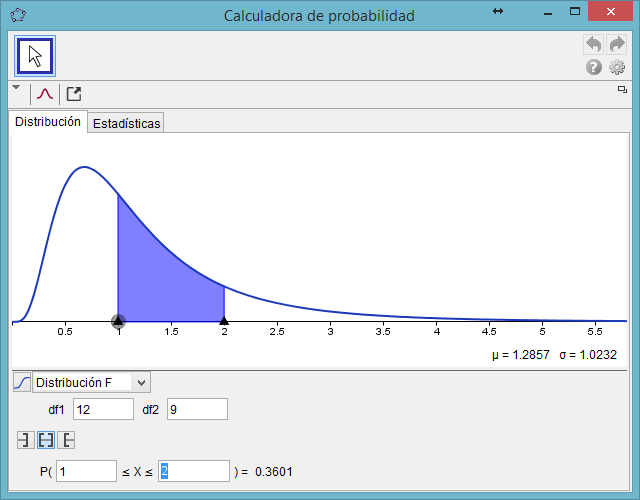
\includegraphics[width=11cm]{../fig/Tut09-04.png}
    \end{center}

\begin{ejercicio}
\label{tut09:ejercicio03}
Repite con GeoGebra los cálculos de probabilidades (directas e inversas) que hemos hecho antes con R.
%\begin{enumerate}
%    \item[]
%    \item
%\end{enumerate}
Solución en la página \pageref{tut09:ejercicio03:sol}.
\qed
\end{ejercicio}


\subsubsection*{En Wolfram Alpha y Calc.}

Para trabajar en Wolfram Alpha puedes usar comandos como los de estos dos ejemplos que, con ligeras modificaciones, cubren todas nuestras necesidades. Para un problema directo usamos algo  como esto:
\begin{center}
\verb# P(X > 3) for X ~ F(13,8)#
\end{center}
y para un problema inverso, por ejemplo para calcular el valor $K$ tal que
\[ P( F_{12;16} < K) = 0.975\]
usaríamos este comando:
\begin{center}
  {\tt 97.5th percentile  for F(12, 16)}
\end{center}
{\bf ¡Ten en cuenta que la probabilidad se ha traducido en percentiles!}

Y, finalmente, no queremos dejar de mencionar las funciones {\tt DISTR.F} y {\tt DISTR.F.INV} de Calc, que permiten trabajar con esta distribución en la hoja de cálculo.


\subsection{Contrastes e intervalos de confianza sobre cocientes de varianzas.}

Ahora que ya sabemos cómo trabajar con la distribución $F$ de Fisher podemos usarla para hacer contrastes de hipótesis e intervalos de confianza relativos al cociente de varianzas. Recuerda que el estadístico adecuado para esos contrastes es:
\[\Xi = \dfrac{s_1^2}{s_2 ^2},\]
y que en la Tabla \ref{curso-tabla:ContrasteHipotesisCocienteVarianzas} del libro (pág. \pageref{curso-tabla:ContrasteHipotesisCocienteVarianzas}) tienes la información necesaria para saber cómo usar el valor del estadístico $\Xi^2$ para calcular el p-valor del contraste.

Antes de hacer algunos ejemplos, unas observaciones genéricas sobre las herramientas de las que disponemos:

\begin{itemize}
  \item A nuestro juicio, y para las versiones actuales del software que usamos, la opción más ventajosa para hacer este tipo de contrastes con la menor cantidad de errores es usar la plantilla de R que hemos incluido en la Tabla \ref{Tut09:tabla:FicherosContrastesDosPoblaciones} de este tutorial (pág. \pageref{Tut09:tabla:FicherosContrastesDosPoblaciones}).
  \item Siguiendo con R, la función {\tt var.test} es especialmente interesante si trabajamos con muestras {\em en bruto}.
  \item En GeoGebra, la {\em Calculadora de Probabilidades} no permite hacer este tipo de contrastes y tampoco hay un comando que se pueda usar directamente en la {\em Línea de Entrada} o el panel de {\em Cálculo Simbólico}. A fecha de hoy, la única forma de hacer este contraste es calculando directamente el p-valor mediante un problema directo de probabilidad con la $F$ de Fisher. En Wolfram Alpha, hasta donde sabemos, sucede algo similar: no hay una herramienta específica para este tipo de contrastes.
\end{itemize}

\subsubsection*{Un ejemplo básico de contrastes de cocientes de varianzas.}

Vamos a supone que estamos estudiando una variable $X$ en dos poblaciones normales $N(\mu_1, \sigma_1)$ y $N(\mu_2, \sigma_2)$ y queremos contrastar la hipótesis alternativa bilateral:
\[H_a = \{\sigma_1 ^2 = \sigma_2^2\}.\]
Para ello hemos tomado muestras aleatorias independientes en cada una de las poblaciones y hemos obtenido estos valores muestrales:



\[
\begin{cases}
n_1 = 59\\[3mm]
s_1 = 3.1
\end{cases}
\qquad
\begin{cases}
n_2 = 64\\[3mm]
s_2 = 4.5
\end{cases}
\]


Para hacer este contraste de la forma más rápida posible, lo más recomendable es usar la plantilla de R de la Tabla \ref{Tut09:tabla:FicherosContrastesDosPoblaciones}. Incluimos aquí las primeras líneas de esa plantilla con los datos que debes introducir:

\begin{knitrout}
\definecolor{shadecolor}{rgb}{0.969, 0.969, 0.969}\color{fgcolor}\begin{kframe}
\begin{alltt}
 \hlcom{# PRIMERA MUESTRA}
 \hlcom{# Numero de elementos}
 \hlstd{(n1} \hlkwb{=} \hlnum{59}\hlstd{)}
\end{alltt}
\begin{verbatim}
## [1] 59
\end{verbatim}
\begin{alltt}
 \hlcom{# Cuasidesviacion tipica muestral}
 \hlstd{(s1} \hlkwb{=} \hlnum{3.1}\hlstd{)}
\end{alltt}
\begin{verbatim}
## [1] 3.1
\end{verbatim}
\begin{alltt}
 \hlcom{# SEGUNDA MUESTRA}
 \hlcom{# Numero de elementos}
 \hlstd{(n2} \hlkwb{=}  \hlnum{64}\hlstd{)}
\end{alltt}
\begin{verbatim}
## [1] 64
\end{verbatim}
\begin{alltt}
 \hlcom{# Cuasidesviacion tipica  muestral}
 \hlstd{(s2} \hlkwb{=} \hlnum{4.5}\hlstd{)}
\end{alltt}
\begin{verbatim}
## [1] 4.5
\end{verbatim}
\begin{alltt}
 \hlcom{# TIPO DE CONTRASTE:}
 \hlcom{# Escribe 1 si la HIP. ALTERNATIVA es sigma > sigma2,}
 \hlcom{#         2 si es sigma1 < sigma2,}
 \hlcom{#         3 si es bilateral.}
 \hlstd{TipoContraste} \hlkwb{=} \hlnum{3}

 \hlcom{#NIVEL DE SIGNIFICACION:}
 \hlstd{(nSig} \hlkwb{=} \hlnum{0.95}\hlstd{)}
\end{alltt}
\begin{verbatim}
## [1] 0.95
\end{verbatim}
\end{kframe}
\end{knitrout}



Y los resultados que se obtienen al ejecutar el fichero son:
\begin{knitrout}
\definecolor{shadecolor}{rgb}{0.969, 0.969, 0.969}\color{fgcolor}\begin{kframe}
\begin{alltt}
     \hlkwd{pValor}\hlstd{(Estadistico,TipoContraste)}
\end{alltt}
\begin{verbatim}
## [1] "El p-Valor es 0.00459021398523596"
\end{verbatim}
\begin{alltt}
     \hlstd{Estadistico}
\end{alltt}
\begin{verbatim}
## [1] 0.47457
\end{verbatim}
\end{kframe}
\end{knitrout}
Así que, por ejemplo, para un nivel de significación del $99\%$ rechazaríamos la hipótesis nula y concluiríamos que los datos no permiten afirmar que las varianzas sean iguales.

\subsubsection*{Y un intervalo de confianza.}

Análogamente, la forma más rápida de obtener elintervalo de confianza es usando la plantilla que aparece al final de este tutorial, en la Tabla \ref{Tut09:tabla:FicherosContrastesDosPoblaciones}. Vamos a usarla para calcular un intervalo de confianza al $95\%$ para los mismos datos que acabamos de usar para el contraste. El código de la plantilla para ese ejemplo es este:

\begin{knitrout}
\definecolor{shadecolor}{rgb}{0.969, 0.969, 0.969}\color{fgcolor}\begin{kframe}
\begin{alltt}
\hlcom{####################################################}
\hlcom{# www.postdata-statistics.com}
\hlcom{# POSTDATA. Introducción a la Estadísitica}
\hlcom{# Tutorial-09.}
\hlcom{#}
\hlcom{# Fichero de instrucciones R para calcular un}
\hlcom{# INTERVALO DE CONFIANZA PARA EL COCIENTE DE VARIANZAS}
\hlcom{# al nivel (1-alfa)   en dos poblaciones normales.}
\hlcom{#}
\hlcom{# El fichero no funcionara si no introduces todos los datos.}
\hlcom{##############################################################}


\hlcom{# Introducimos los valores de las desviaciones tipicas muestrales,}
\hlstd{s1} \hlkwb{=} \hlnum{3.1}
\hlstd{s2} \hlkwb{=} \hlnum{4.5}


\hlcom{# los tamaños de las muestras,}
\hlstd{n1} \hlkwb{=} \hlnum{59}
\hlstd{n2} \hlkwb{=} \hlnum{64}

\hlcom{# y el nivel de confianza deseado.}
\hlstd{nc} \hlkwb{=} \hlnum{0.95}

\hlcom{## --- NO CAMBIES NADA DE AQUI PARA ABAJO}

\hlstd{(alfa} \hlkwb{=} \hlnum{1} \hlopt{-} \hlstd{nc)}
\end{alltt}
\begin{verbatim}
## [1] 0.05
\end{verbatim}
\begin{alltt}
\hlcom{# Calculamos los valor criticos necesarios:}

\hlstd{(f_alfamedios} \hlkwb{=} \hlkwd{qf}\hlstd{(alfa}\hlopt{/}\hlnum{2}\hlstd{,} \hlkwc{df1}\hlstd{=n1} \hlopt{-} \hlnum{1}\hlstd{,} \hlkwc{df2}\hlstd{=n2} \hlopt{-} \hlnum{1}\hlstd{))}
\end{alltt}
\begin{verbatim}
## [1] 0.59935
\end{verbatim}
\begin{alltt}
\hlstd{(f_unomenosalfamedios} \hlkwb{=} \hlkwd{qf}\hlstd{(}\hlnum{1} \hlopt{-} \hlstd{alfa}\hlopt{/}\hlnum{2}\hlstd{,} \hlkwc{df1}\hlstd{=n1} \hlopt{-} \hlnum{1}\hlstd{,} \hlkwc{df2}\hlstd{= n2}\hlopt{-}\hlnum{1}\hlstd{))}
\end{alltt}
\begin{verbatim}
## [1] 1.6594
\end{verbatim}
\begin{alltt}
\hlcom{# El intervalo de confianza para el cociente de varianzas es este:}
\hlstd{(intervalo} \hlkwb{=} \hlkwd{c}\hlstd{( (}\hlnum{1}\hlopt{/}\hlstd{f_unomenosalfamedios), (}\hlnum{1}\hlopt{/}\hlstd{f_alfamedios))} \hlopt{*} \hlstd{(s1}\hlopt{^}\hlnum{2}\hlopt{/}\hlstd{s2}\hlopt{^}\hlnum{2}\hlstd{))}
\end{alltt}
\begin{verbatim}
## [1] 0.28598 0.79180
\end{verbatim}
\end{kframe}
\end{knitrout}

Podemos aprovechar este cálculo para confirmar las conclusiones del contraste: puesto que el intervalo no contiene al $1$, estamos en condiciones de rechazar $H_0$ al $95\%$.


% \subsubsection*{A partir de datos en bruto.}
%
% Para nuestro segundo ejemplo vamos a suponer que los datos están en un fichero {\tt csv}.
%
% <<tut09-ejemploContrasteCocienteVarianzas02, echo=FALSE, results='hide'>>=
% <<tut09-ejemploContrasteCocienteVarianzas01>>
% library(MASS)
% set.seed(2014)
% muestra1 = as.vector(mvrnorm(n = n1, mu = 2.5, Sigma = s1^2, empirical = TRUE))
% muestra2 = as.vector(mvrnorm(n = n2, mu = 3.6, Sigma = s2^2, empirical = TRUE))
% length(muestra1) <- max(length(muestra1), length(muestra2))
% length(muestra2) <- max(length(muestra1), length(muestra2))
%
% datos = data.frame(muestra1, muestra2)
% write.table(datos, "../datos/Tut09-EjemCtrsteVarianzas-DatosEnBruto-FichMal.csv", row.names = FALSE, col.names = c("muestra1", "muestra2"))
% @
%
% Claro está, al tratarse de dos muestras, el fichero debe contener los datos de ambas muestras. Y esohace que este fichero sea especial en varios sentidos, comparado con otros ficheros Hay dos formas posibles para el fichero.


\section{Diferencia de medias en dos poblaciones, muestras pequeñas.}
\label{tut09:sec:DiferenciaMedias2PoblacionesPequennas}


\subsection{Los contrastes de los ejemplos de la Sección \ref{curso-cap09:subsec:EjemplosContrasteDiferenciaMediasUsandoT} del libro.}


Vamos a empezar mostrando como comprobar los datos de esos ejemplos usando R. En todos los casos es necesario realizar un contraste previo de varianzas, para luego pasar al contraste de diferencia de medias. La forma más rápida de proceder es usando las plantillas de R. Concretamente, usaremos la plantilla
\begin{center}
  {\tt Tut09-Contraste-2Pob-CocienteVarianzas.R}
\end{center}
para los contrastes sobre cocientes de varianzas y después usaremos una de las plantillas
\begin{center}
  {\tt Tut09-Contraste-2Pob-DifMedias-UsandoT-VarDistintas.R}\\
  {\tt Tut09-Contraste-2Pob-DifMedias-UsandoT-VarIguales.R}
\end{center}

\subsubsection*{Ejemplo \ref{curso-cap09:ejem:ContrasteDiferenciaMediasVarianzasIguales}}
Empezamos por este ejemplo, que aparece en la página \pageref{curso-cap09:ejem:ContrasteDiferenciaMediasVarianzasIguales} del libro. Allí puedes ver los valores necesarios, así que sólo mostraremos el principio del código de la plantilla que usamos para el contraste de varianzas. Ten en cuenta que puede haber pequeños discrepancias con respecto a los valores del libro debidos al redondeo, porque aquí no estamos tomando como partida los datos en bruto que aparecen en el ejemplo:

\begin{knitrout}
\definecolor{shadecolor}{rgb}{0.969, 0.969, 0.969}\color{fgcolor}\begin{kframe}
\begin{alltt}
 \hlcom{# PRIMERA MUESTRA}
 \hlcom{# Numero de elementos}
 \hlstd{(n1} \hlkwb{=} \hlnum{10}\hlstd{)}
\end{alltt}
\begin{verbatim}
## [1] 10
\end{verbatim}
\begin{alltt}
 \hlcom{# Cuasidesviacion tipica muestral}
 \hlstd{(s1} \hlkwb{=} \hlnum{2.098}\hlstd{)}
\end{alltt}
\begin{verbatim}
## [1] 2.098
\end{verbatim}
\begin{alltt}
 \hlcom{# SEGUNDA MUESTRA}
 \hlcom{# Numero de elementos}
 \hlstd{(n2} \hlkwb{=} \hlnum{10}\hlstd{)}
\end{alltt}
\begin{verbatim}
## [1] 10
\end{verbatim}
\begin{alltt}
 \hlcom{# Cuasidesviacion tipica  muestral}
 \hlstd{(s2} \hlkwb{=} \hlnum{2.111}\hlstd{)}
\end{alltt}
\begin{verbatim}
## [1] 2.111
\end{verbatim}
\begin{alltt}
 \hlcom{# TIPO DE CONTRASTE:}
 \hlcom{# Escribe 1 si la HIP. ALTERNATIVA es sigma > sigma2,}
 \hlcom{#         2 si es sigma1 < sigma2,}
 \hlcom{#         3 si es bilateral.}
 \hlstd{TipoContraste} \hlkwb{=} \hlnum{3}

 \hlcom{#NIVEL DE SIGNIFICACION:}
 \hlstd{(nSig} \hlkwb{=} \hlnum{0.95}\hlstd{)}
\end{alltt}
\begin{verbatim}
## [1] 0.95
\end{verbatim}
\end{kframe}
\end{knitrout}



Y los resultados que obtenemos:
\begin{knitrout}
\definecolor{shadecolor}{rgb}{0.969, 0.969, 0.969}\color{fgcolor}\begin{kframe}
\begin{alltt}
 \hlcom{# Y ahora se aplican ambas funciones para mostrar los resultados}
     \hlkwd{pValor}\hlstd{(Estadistico,TipoContraste)}
\end{alltt}
\begin{verbatim}
## [1] "El p-Valor es 0.985618870598065"
\end{verbatim}
\begin{alltt}
     \hlstd{Estadistico}
\end{alltt}
\begin{verbatim}
## [1] 0.98772
\end{verbatim}
\end{kframe}
\end{knitrout}
Como puedes ver y salvo la pequeña discrepancia numérica, confirmamos  la conclusión que aparece en el texto: no tenemos razones para pensar que las varianzas sean distintas. Así que de las dos posibles usamos la plantilla {\tt Tut09-Contraste-2Pob-DifMedias-UsandoT-VarIguales.R}. Vamos a ver la parte inicial del código de esa plantilla, con los datos del problema. Ten en cuenta, insistimos, que puede haber pequeñas discrepancias numéricas con los valores que aparecen en el libro. Además en este ejemplo estamos llamando $\mu_t, \mu_b$ a lo que normalmente llamamos $\{\mu_1, \mu_2\}$. Ten presente esto a la hora de elegir el tipo de contraste.

\begin{knitrout}
\definecolor{shadecolor}{rgb}{0.969, 0.969, 0.969}\color{fgcolor}\begin{kframe}
\begin{alltt}
 \hlcom{# PRIMERA MUESTRA # Numero de elementos}
 \hlstd{(n1} \hlkwb{=} \hlnum{10}\hlstd{)}
\end{alltt}
\begin{verbatim}
## [1] 10
\end{verbatim}
\begin{alltt}
 \hlcom{# Media muestral}
 \hlstd{(xbar1} \hlkwb{=} \hlnum{94.2}\hlstd{)}
\end{alltt}
\begin{verbatim}
## [1] 94.2
\end{verbatim}
\begin{alltt}
 \hlcom{# Cuasidesviacion tipica muestral}
 \hlstd{(s1} \hlkwb{=} \hlnum{2.098}\hlstd{)}
\end{alltt}
\begin{verbatim}
## [1] 2.098
\end{verbatim}
\begin{alltt}
 \hlcom{# SEGUNDA MUESTRA}
 \hlcom{# Numero de elementos}
 \hlstd{(n2} \hlkwb{=} \hlnum{10}\hlstd{)}
\end{alltt}
\begin{verbatim}
## [1] 10
\end{verbatim}
\begin{alltt}
 \hlcom{# Media muestral}
 \hlstd{(xbar2} \hlkwb{=} \hlnum{97.7}\hlstd{)}
\end{alltt}
\begin{verbatim}
## [1] 97.7
\end{verbatim}
\begin{alltt}
 \hlcom{# Cuasidesviacion tipica  muestral}
 \hlstd{(s2} \hlkwb{=} \hlnum{2.111}\hlstd{)}
\end{alltt}
\begin{verbatim}
## [1] 2.111
\end{verbatim}
\begin{alltt}
 \hlcom{# ¿Que tipo de contraste estamos haciendo?}
 \hlcom{# Escribe 1 si la HIP. ALTERNATIVA es mu1 > mu2, 2 si es mu1 < mu2, 3 si es mu1 distinto de mu2}
     \hlstd{TipoContraste} \hlkwb{=} \hlnum{2}
 \hlcom{#Nivel de significacion}
     \hlstd{(nSig} \hlkwb{=} \hlnum{0.95}\hlstd{)}
\end{alltt}
\begin{verbatim}
## [1] 0.95
\end{verbatim}
\end{kframe}
\end{knitrout}





Los resultados son:
\begin{knitrout}
\definecolor{shadecolor}{rgb}{0.969, 0.969, 0.969}\color{fgcolor}\begin{kframe}
\begin{alltt}
     \hlkwd{pValor}\hlstd{(Estadistico, TipoContraste)}
\end{alltt}
\begin{verbatim}
## [1] "El p-Valor es 0.000785741251043506"
\end{verbatim}
\begin{alltt}
     \hlstd{Estadistico}
\end{alltt}
\begin{verbatim}
## [1] -3.7188
\end{verbatim}
\begin{alltt}
     \hlkwd{RegionRechazo}\hlstd{(alfa, TipoContraste)}
\end{alltt}
\begin{verbatim}
## [1] "La region de rechazo la forman los Valores del Estadistico menores que  -1.73406360661754"
\end{verbatim}
\end{kframe}
\end{knitrout}
respaldando las conclusiones que hemos obtenido en este ejemplo.

\subsubsection*{Ejemplo \ref{curso-cap09:ejem:ContrasteDiferenciaMediasVarianzasIguales}}

Este ejemplo aparece en la pág. \ref{curso-cap09:ejem:ContrasteDiferenciaMediasVarianzasDistintas} del libro. Como en el anterior, empezamos con el código necesario para el contraste de varianzas. El comienzo de la plantilla sería así:

\begin{knitrout}
\definecolor{shadecolor}{rgb}{0.969, 0.969, 0.969}\color{fgcolor}\begin{kframe}
\begin{alltt}
 \hlcom{# PRIMERA MUESTRA}
 \hlcom{# Numero de elementos}
 \hlstd{(n1} \hlkwb{=} \hlnum{12}\hlstd{)}
\end{alltt}
\begin{verbatim}
## [1] 12
\end{verbatim}
\begin{alltt}
 \hlcom{# Cuasidesviacion tipica muestral}
 \hlstd{(s1} \hlkwb{=} \hlnum{0.4216}\hlstd{)}
\end{alltt}
\begin{verbatim}
## [1] 0.4216
\end{verbatim}
\begin{alltt}
 \hlcom{# SEGUNDA MUESTRA}
 \hlcom{# Numero de elementos}
 \hlstd{(n2} \hlkwb{=} \hlnum{12}\hlstd{)}
\end{alltt}
\begin{verbatim}
## [1] 12
\end{verbatim}
\begin{alltt}
 \hlcom{# Cuasidesviacion tipica  muestral}
 \hlstd{(s2} \hlkwb{=} \hlnum{0.1740}\hlstd{)}
\end{alltt}
\begin{verbatim}
## [1] 0.174
\end{verbatim}
\begin{alltt}
 \hlcom{# TIPO DE CONTRASTE:}
 \hlcom{# Escribe 1 si la HIP. ALTERNATIVA es sigma > sigma2,}
 \hlcom{#         2 si es sigma1 < sigma2,}
 \hlcom{#         3 si es bilateral.}
 \hlstd{TipoContraste} \hlkwb{=} \hlnum{3}

 \hlcom{#NIVEL DE SIGNIFICACION:}
 \hlstd{(nSig} \hlkwb{=} \hlnum{0.95}\hlstd{)}
\end{alltt}
\begin{verbatim}
## [1] 0.95
\end{verbatim}
\end{kframe}
\end{knitrout}



Y los resultados que obtenemos:
\begin{knitrout}
\definecolor{shadecolor}{rgb}{0.969, 0.969, 0.969}\color{fgcolor}\begin{kframe}
\begin{alltt}
 \hlcom{# Y ahora se aplican ambas funciones para mostrar los resultados}
     \hlkwd{pValor}\hlstd{(Estadistico,TipoContraste)}
\end{alltt}
\begin{verbatim}
## [1] "El p-Valor es 0.00666781125885452"
\end{verbatim}
\begin{alltt}
     \hlstd{Estadistico}
\end{alltt}
\begin{verbatim}
## [1] 5.8709
\end{verbatim}
\end{kframe}
\end{knitrout}
En este caso, como el punto de partida son los propios valores que se han usado en el libro, no hay errores de redondeo apreciables. La conclusión, como se explica en el libro, es que rechazamos la hipótesis nula de igualdad de varianzas.

Por tanto, de vuelta al contraste de medias, vamos a usar la plantilla de la Tabla \ref{Tut09:tabla:FicherosContrastesDosPoblaciones} titulada
\begin{center}
{\tt Tut09-Contraste-2Pob-DifMedias-UsandoT-VarIguales.R}
\end{center}
Ten en cuenta además la notación $H_a = \{\mu_2 - \mu_3\}$ que se ha usado en este ejemplo, a la hora de seleccionar el tipo de contraste. Con los datos del ejemplo, la primera parte de esa plantilla quedaría así:

{\small
\begin{knitrout}
\definecolor{shadecolor}{rgb}{0.969, 0.969, 0.969}\color{fgcolor}\begin{kframe}
\begin{alltt}
 \hlcom{# PRIMERA MUESTRA # Numero de elementos}
 \hlstd{(n1} \hlkwb{=} \hlnum{12}\hlstd{)}
\end{alltt}
\begin{verbatim}
## [1] 12
\end{verbatim}
\begin{alltt}
 \hlcom{# Media muestral}
 \hlstd{(xbar1} \hlkwb{=} \hlnum{1.914}\hlstd{)}
\end{alltt}
\begin{verbatim}
## [1] 1.914
\end{verbatim}
\begin{alltt}
 \hlcom{# Cuasidesviacion tipica muestral}
 \hlstd{(s1} \hlkwb{=} \hlnum{0.4216}\hlstd{)}
\end{alltt}
\begin{verbatim}
## [1] 0.4216
\end{verbatim}
\begin{alltt}
 \hlcom{# SEGUNDA MUESTRA}
 \hlcom{# Numero de elementos}
 \hlstd{(n2} \hlkwb{=} \hlnum{12}\hlstd{)}
\end{alltt}
\begin{verbatim}
## [1] 12
\end{verbatim}
\begin{alltt}
 \hlcom{# Media muestral}
 \hlstd{(xbar2} \hlkwb{=} \hlnum{2.344}\hlstd{)}
\end{alltt}
\begin{verbatim}
## [1] 2.344
\end{verbatim}
\begin{alltt}
 \hlcom{# Cuasidesviacion tipica  muestral}
 \hlstd{(s2} \hlkwb{=} \hlnum{0.1740}\hlstd{)}
\end{alltt}
\begin{verbatim}
## [1] 0.174
\end{verbatim}
\begin{alltt}
\hlcom{# ¿Que tipo de contraste estamos haciendo?}
\hlcom{# Escribe:    1 si la HIP. ALTERNATIVA es mu1 > mu2,}
\hlcom{#             2 si es mu1 < mu2,}
\hlcom{#             3 si es mu1 distinto de mu2}
\hlstd{TipoContraste} \hlkwb{=} \hlnum{2}

\hlcom{#Nivel de significacion}
\hlstd{(nSig} \hlkwb{=} \hlnum{0.95}\hlstd{)}
\end{alltt}
\begin{verbatim}
## [1] 0.95
\end{verbatim}
\end{kframe}
\end{knitrout}



En este caso vamos a mostrar el número de grados de libertad que se obtienen usando la aproximación de Welch:

\begin{knitrout}
\definecolor{shadecolor}{rgb}{0.969, 0.969, 0.969}\color{fgcolor}\begin{kframe}
\begin{alltt}
 \hlcom{# Grados de libertad, aproximacion de Welch}
 \hlstd{(k} \hlkwb{=} \hlstd{(s1}\hlopt{^}\hlnum{2}\hlopt{/}\hlstd{n1} \hlopt{+} \hlstd{s2}\hlopt{^}\hlnum{2}\hlopt{/}\hlstd{n2)}\hlopt{^}\hlnum{2} \hlopt{/} \hlstd{((s1}\hlopt{^}\hlnum{4}\hlopt{/}\hlstd{(n1}\hlopt{^}\hlnum{2} \hlopt{*} \hlstd{(n1} \hlopt{-} \hlnum{1}\hlstd{)))} \hlopt{+} \hlstd{(s2}\hlopt{^}\hlnum{4} \hlopt{/} \hlstd{(n2}\hlopt{^}\hlnum{2} \hlopt{*} \hlstd{(n2} \hlopt{-} \hlnum{1}\hlstd{)))))}
\end{alltt}
\begin{verbatim}
## [1] 14.642
\end{verbatim}
\end{kframe}
\end{knitrout}



}

Los resultados son:
{\small
\begin{knitrout}
\definecolor{shadecolor}{rgb}{0.969, 0.969, 0.969}\color{fgcolor}\begin{kframe}
\begin{alltt}
     \hlkwd{pValor}\hlstd{(Estadistico, TipoContraste)}
\end{alltt}
\begin{verbatim}
## [1] "El p-Valor es 0.002676528260678"
\end{verbatim}
\begin{alltt}
     \hlstd{Estadistico}
\end{alltt}
\begin{verbatim}
## [1] -3.2659
\end{verbatim}
\begin{alltt}
     \hlkwd{RegionRechazo}\hlstd{(alfa, TipoContraste)}
\end{alltt}
\begin{verbatim}
## [1] "La region de rechazo la forman los valores del Estadistico menores que  -1.75587212046059"
\end{verbatim}
\end{kframe}
\end{knitrout}
}

\vspace{-3mm}
\noindent{\bf Contrastes de diferencia de medias con GeoGebra en el caso de muestras pequeñas.}\\[3mm]
La {\em Calculadora de Probabilidades} de GeoGebra incluye, en la pestaña titulada {\em Estadísticas}, la opción de calcular estos contrastes de diferencia de medias, introduciendo los valores muestrales en los campos del formulario que se muestra. Para revisar el funcionamiento de esta herramienta vamos a usar los datos de los dos ejemplos que hemos hecho antes con las plantillas de R y luego comentaremos algunos aspectos particulares. En esta primera figura se ilustra la forma de obtener el contraste del Ejemplo \ref{curso-cap09:ejem:ContrasteDiferenciaMediasVarianzasIguales} del libro.

\begin{center}
    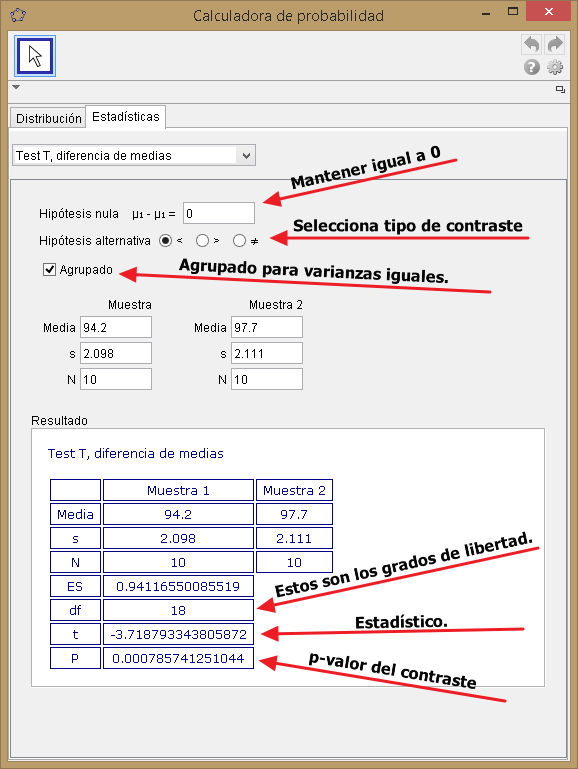
\includegraphics[width=10cm]{../fig/Tut09-05.png}
\end{center}

Mientras que para el Ejemplo \ref{curso-cap09:ejem:ContrasteDiferenciaMediasVarianzasDistintas} del libro debemos proceder como se muestra en esta figura:

\begin{center}
    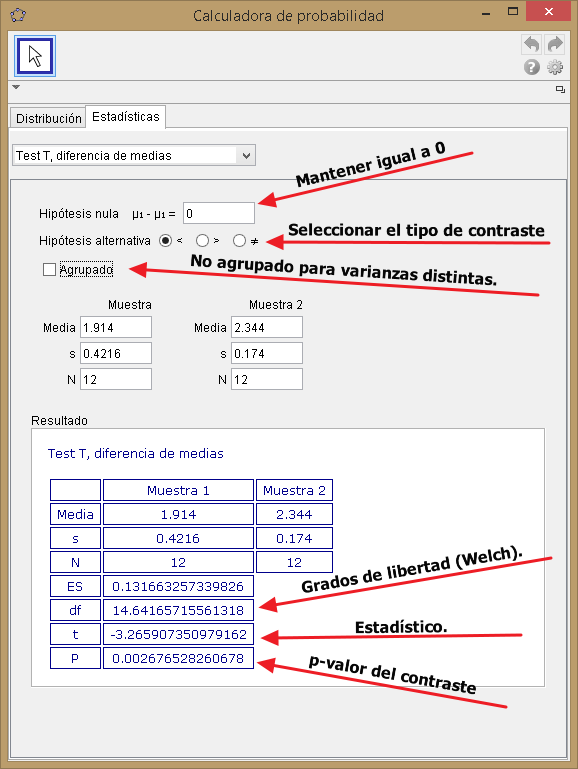
\includegraphics[width=10cm]{../fig/Tut09-06.png}
\end{center}

Vamos a comentar algunos aspectos reseñables de esta herramienta:

\begin{itemize}
  \item Aunque GeoGebra es un programa que las más de las veces resulta intuitivo y fácil de usar, esta interfaz no es, tal vez, de las más conseguidas. En la versión actual se ha colado además una errata que hace que en la hipótesis nula aparezca la fórmula $\mu_1 - \mu_1$ donde debería decir $\mu_1 - \mu_2$. Esta diferencia aparece igualada inicialmente a $0$, aunque ese valor puede modificarse, para dar cabida a posibles hipótesis nulas como, por ejemplo (también podría ser con $\geq$ o $=$):
        \[H_0 = \{(\mu_1-\mu_2)\leq \Delta \mu_0\}\]
      donde $\Delta \mu_0$ es una cantidad dada, en el mismo sentido que hemos discutido, para el caso de proporciones, en la Sección \ref{curso-cap09:subsec:ContrasteHipotesisDiferenciaProporciones} del libro (pág. \pageref{curso-cap09:subsec:ContrasteHipotesisDiferenciaProporciones}). En particular eso significa que {\bf en la mayoría de las ocasiones queremos mantener el valor $\mu_1 - \mu_2 = 0$}.
  \item Los programadores de GeoGebra usan descripciones de la hipótesis nula que podemos resumir en la forma:
        \[H_a = \{\mu_1 - \mu_2 \,\bigstar\, 0\}\]
        donde $\,\bigstar\,$ es un símbolo que puede ser $<$, $>$ 0 $\neq$. Pero hay que tener en cuenta que, por ejemplo
        \[H_a = \{\mu_1 - \mu_2 < 0\} = \{\mu_1 < \mu_2\}.\]
        Así que decir que $\mu_1 - \mu_2 \,\bigstar\, 0$ es lo mismo que decir $\mu_1 \,\bigstar\,  \mu_2 $ {\em sea cual sea la interpretación del símbolo } $\,\bigstar\,$ de entre las tres posibles.
  \item Para elegir entre el caso en que asumimos varianzas iguales y el caso de varianzas distintas, debemos usar la casilla titulada {\em Agrupado}. Como hemos indicado en las figuras, marcamos esa casilla para el caso de varianzas iguales y la dejamos sin marcar en el caso de varianzas distintas.

\end{itemize}

\subsection{Intervalos de confianza para la diferencia de medias con R.}

Vamos a calcular intervalos de confianza al $95\%$ para la diferencia $\mu_1 - \mu_2$ en los Ejemplos \ref{curso-cap09:ejem:ContrasteDiferenciaMediasVarianzasIguales} y \ref{curso-cap09:ejem:ContrasteDiferenciaMediasVarianzasDistintas} del libro que estamos usando en estos últimos apartados. Para ello usaremos los dos ficheros plantilla de la Tabla \ref{Tut09:tabla:FicherosContrastesDosPoblaciones}.

Para el Ejemplo \ref{curso-cap09:ejem:ContrasteDiferenciaMediasVarianzasIguales} usamos el fichero {\tt Tut09-IntConf-2Pob-DifMedias-UsandoT-VarianzasIguales.R}. El código con los datos del ejemplo sería así:

\begin{knitrout}
\definecolor{shadecolor}{rgb}{0.969, 0.969, 0.969}\color{fgcolor}\begin{kframe}
\begin{alltt}
\hlcom{####################################################}
\hlcom{# www.postdata-statistics.com}
\hlcom{# POSTDATA. Introducción a la Estadísitica}
\hlcom{# Tutorial-09.}
\hlcom{#}
\hlcom{# Fichero de instrucciones R para calcular}
\hlcom{# un intervalo de confianza para la}
\hlcom{# DIFERENCIA DE MEDIAS DE 2 POBLACIONES NORMALES}
\hlcom{# Es el caso de}
\hlcom{# MUESTRAS PEQUEÑAS}
\hlcom{# bajo la hipotesis de}
\hlcom{# VARIANZAS IGUALES.}
\hlcom{##############################################################}

\hlcom{# Introducimos los tamaños de las muestras:}
\hlstd{n1} \hlkwb{=} \hlnum{10}
\hlstd{n2} \hlkwb{=} \hlnum{10}
\hlcom{# Medias muestrales:}
\hlstd{barX1} \hlkwb{=} \hlnum{94.2}
\hlstd{barX2} \hlkwb{=} \hlnum{97.7}
\hlcom{# Cuasidesviaciones tipicas muestrales:}
\hlstd{s1} \hlkwb{=} \hlnum{2.098}
\hlstd{s2} \hlkwb{=} \hlnum{2.111}

\hlcom{# Nivel de confianza deseado:}
\hlstd{nc} \hlkwb{=} \hlnum{0.95}

\hlcom{################################################}
\hlcom{#NO CAMBIES NADA DE AQUI PARA ABAJO}
\hlcom{################################################}
\hlcom{# Calculamos los grados de libertad:}
\hlstd{(k} \hlkwb{=} \hlstd{n1} \hlopt{+} \hlstd{n2} \hlopt{-} \hlnum{2}\hlstd{)}
\end{alltt}
\begin{verbatim}
## [1] 18
\end{verbatim}
\begin{alltt}
\hlcom{# Calculamos el valor critico:}
\hlstd{(alfa} \hlkwb{=} \hlnum{1} \hlopt{-} \hlstd{nc)}
\end{alltt}
\begin{verbatim}
## [1] 0.05
\end{verbatim}
\begin{alltt}
\hlstd{(t_alfa2} \hlkwb{=} \hlkwd{qt}\hlstd{(}\hlnum{1} \hlopt{-} \hlstd{alfa}\hlopt{/}\hlnum{2}\hlstd{,} \hlkwc{df}\hlstd{=k))}
\end{alltt}
\begin{verbatim}
## [1] 2.1009
\end{verbatim}
\begin{alltt}
\hlcom{# La semianchura del intervalo es}
\hlstd{(semianchura} \hlkwb{=} \hlstd{t_alfa2} \hlopt{*} \hlkwd{sqrt}\hlstd{((((n1} \hlopt{-} \hlnum{1}\hlstd{)} \hlopt{*} \hlstd{s1}\hlopt{^}\hlnum{2} \hlopt{+} \hlstd{(n2} \hlopt{-} \hlnum{1}\hlstd{)} \hlopt{*} \hlstd{s2}\hlopt{^}\hlnum{2}\hlstd{)} \hlopt{/}\hlstd{k)} \hlopt{*} \hlstd{(}\hlnum{1}\hlopt{/}\hlstd{n1} \hlopt{+} \hlnum{1}\hlopt{/}\hlstd{n2)))}
\end{alltt}
\begin{verbatim}
## [1] 1.9773
\end{verbatim}
\begin{alltt}
\hlcom{# Intervalo de confianza}
\hlstd{(intervalo} \hlkwb{=} \hlstd{(barX1} \hlopt{-} \hlstd{barX2)} \hlopt{+} \hlkwd{c}\hlstd{(}\hlopt{-}\hlnum{1}\hlstd{,} \hlnum{1}\hlstd{)} \hlopt{*} \hlstd{semianchura)}
\end{alltt}
\begin{verbatim}
## [1] -5.4773 -1.5227
\end{verbatim}
\end{kframe}
\end{knitrout}

Para el Ejemplo \ref{curso-cap09:ejem:ContrasteDiferenciaMediasVarianzasDistintas} usaremos el fichero {\tt Tut09-IntConf-2Pob-DifMedias-UsandoT-VarianzasDistintas.R}. Con los datos del Ejemplo el código quedaría así:

\begin{knitrout}
\definecolor{shadecolor}{rgb}{0.969, 0.969, 0.969}\color{fgcolor}\begin{kframe}
\begin{alltt}
\hlcom{####################################################}
\hlcom{# www.postdata-statistics.com}
\hlcom{# POSTDATA. Introducción a la Estadísitica}
\hlcom{# Tutorial-09.}
\hlcom{#}
\hlcom{# Fichero de instrucciones R para calcular}
\hlcom{# un intervalo de confianza para la}
\hlcom{# DIFERENCIA DE MEDIAS DE 2 POBLACIONES NORMALES}
\hlcom{# Es el caso de}
\hlcom{# MUESTRAS PEQUEÑAS}
\hlcom{# bajo la hipotesis de}
\hlcom{# VARIANZAS IGUALES.}
\hlcom{##############################################################}

\hlcom{# Introducimos los tamaños de las muestras:}
\hlstd{n1} \hlkwb{=} \hlnum{12}
\hlstd{n2} \hlkwb{=} \hlnum{12}
\hlcom{# Medias muestrales:}
\hlstd{barX1} \hlkwb{=} \hlnum{1.914}
\hlstd{barX2} \hlkwb{=} \hlnum{2.344}
\hlcom{# Cuasidesviaciones tipicas muestrales:}
\hlstd{s1} \hlkwb{=} \hlnum{0.4216}
\hlstd{s2} \hlkwb{=} \hlnum{0.1740}

\hlcom{# Nivel de confianza deseado:}
\hlstd{nc} \hlkwb{=} \hlnum{0.95}

\hlcom{################################################}
\hlcom{#NO CAMBIES NADA DE AQUI PARA ABAJO}
\hlcom{################################################}

\hlcom{# Calculamos los grados de libertad usando la aprox. de Welch}
\hlstd{(k} \hlkwb{=} \hlstd{(s1}\hlopt{^}\hlnum{2}\hlopt{/}\hlstd{n1} \hlopt{+} \hlstd{s2}\hlopt{^}\hlnum{2}\hlopt{/}\hlstd{n2)}\hlopt{^}\hlnum{2} \hlopt{/} \hlstd{((s1}\hlopt{^}\hlnum{4}\hlopt{/}\hlstd{(n1}\hlopt{^}\hlnum{2} \hlopt{*} \hlstd{(n1} \hlopt{-} \hlnum{1}\hlstd{)))} \hlopt{+} \hlstd{(s2}\hlopt{^}\hlnum{4} \hlopt{/} \hlstd{(n2}\hlopt{^}\hlnum{2} \hlopt{*} \hlstd{(n2} \hlopt{-} \hlnum{1}\hlstd{)))))}
\end{alltt}
\begin{verbatim}
## [1] 14.642
\end{verbatim}
\begin{alltt}
\hlcom{# Calculamos el valor critico:}
\hlstd{(alfa} \hlkwb{=} \hlnum{1} \hlopt{-} \hlstd{nc)}
\end{alltt}
\begin{verbatim}
## [1] 0.05
\end{verbatim}
\begin{alltt}
\hlstd{(t_alfa2} \hlkwb{=} \hlkwd{qt}\hlstd{(}\hlnum{1}\hlopt{-}\hlstd{alfa}\hlopt{/}\hlnum{2}\hlstd{,} \hlkwc{df}\hlstd{=k))}
\end{alltt}
\begin{verbatim}
## [1] 2.136
\end{verbatim}
\begin{alltt}
\hlcom{#La semianchura del intervalo es:}
\hlstd{(semianchura} \hlkwb{=} \hlstd{t_alfa2} \hlopt{*} \hlkwd{sqrt}\hlstd{(s1}\hlopt{^}\hlnum{2}\hlopt{/}\hlstd{n1} \hlopt{+} \hlstd{s2}\hlopt{^}\hlnum{2}\hlopt{/}\hlstd{n2))}
\end{alltt}
\begin{verbatim}
## [1] 0.28123
\end{verbatim}
\begin{alltt}
\hlcom{# El intervalo de confianza es:}
\hlstd{(intervalo} \hlkwb{=} \hlstd{(barX1} \hlopt{-} \hlstd{barX2)} \hlopt{+} \hlkwd{c}\hlstd{(}\hlopt{-}\hlnum{1}\hlstd{,} \hlnum{1}\hlstd{)} \hlopt{*} \hlstd{semianchura  )}
\end{alltt}
\begin{verbatim}
## [1] -0.71123 -0.14877
\end{verbatim}
\end{kframe}
\end{knitrout}

\subsubsection*{Con GeoGebra.}

En la {\em Calculadora de Probabilidades} de GeoGebra, podemos usar la opción {\em Intervalo T, diferencia de Medias}. Las siguientes figuras muestran el cálculo de los intervalos que hemos obtenido previamente con R.

\begin{center}
    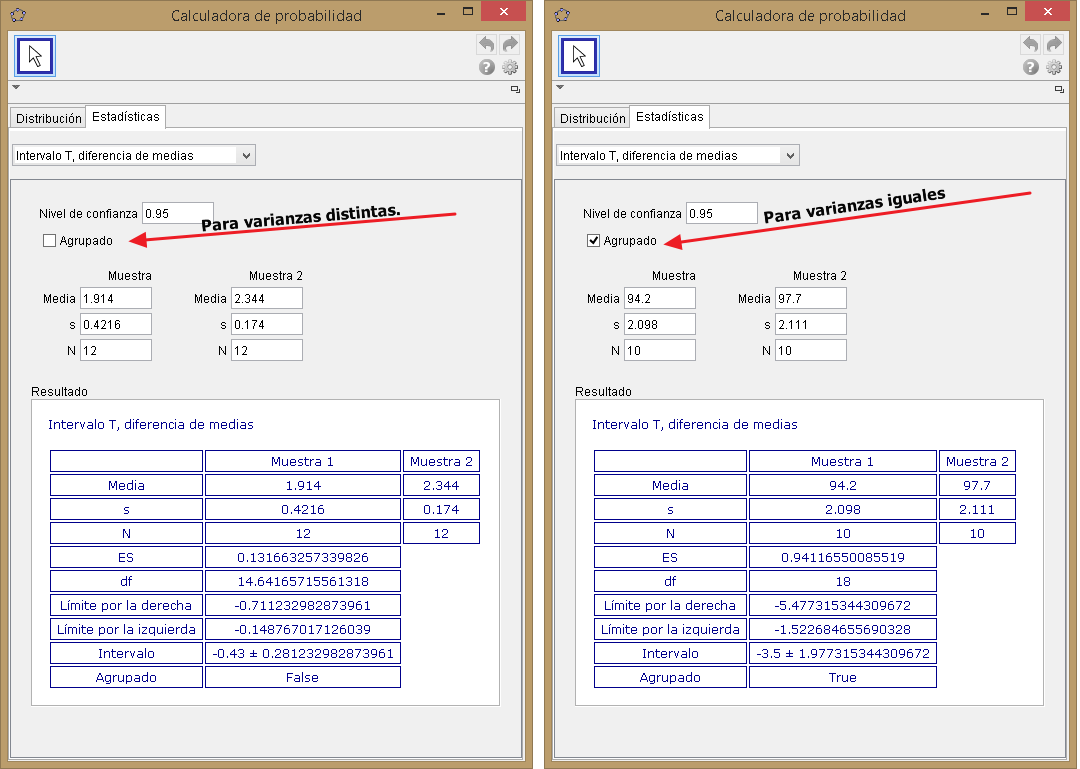
\includegraphics[width=15cm]{../fig/Tut09-07.png}
\end{center}

%%%%%%%%%%%%%%%%%%%%%%%%%%%%%%%%%%%%%%%%%%%%%%%%%%%%%%%%%%%%%%%%%%%%%%%%%%%%%%%%%%%%%%%%%%%%%
%%%%%%%%%%%%%%%%%%%%%%%%%%%%%%%%%%%%%%%%%%%%%%%%%%%%%%%%%%%%%%%%%%%%%%%%%%%%%%%%%%%%%%%%%%%%%
\section{Datos {\em en bruto} con R.}
\label{tut09:sec:DatosEnBrutoconR}
%%%%%%%%%%%%%%%%%%%%%%%%%%%%%%%%%%%%%%%%%%%%%%%%%%%%%%%%%%%%%%%%%%%%%%%%%%%%%%%%%%%%%%%%%%%%%
%%%%%%%%%%%%%%%%%%%%%%%%%%%%%%%%%%%%%%%%%%%%%%%%%%%%%%%%%%%%%%%%%%%%%%%%%%%%%%%%%%%%%%%%%%%%%
\noindent{\bf Opcional: esta sección puede omitirse en una primera lectura. De hecho, para leer esta sección, es necesario haber aprendido previamente a manejar los {\tt data.frame} de R. Se recomienda en particular la lectura de la Sección \ref{tut04-tut04:sec:FicherosDatosRObjetosDataFrame} (pág. \pageref{tut04-tut04:sec:FicherosDatosRObjetosDataFrame}) del Tutorial04.}

Vamos a dedicar esta sección a profundizar en el uso de varias funciones de R que son especialmente útiles para realizar contrastes entre parámetros de dos poblaciones. Las funciones son:
\begin{itemize}
  \item {\tt prop.test}
  \item {\tt z.test}
  \item {\tt t.test}
  \item {\tt var.test}
\end{itemize}
Ya hemos discutido la función {\tt prop.test} en la Sección \ref{tut09:subsubsec:FuncionPropTest} (pág. \pageref{tut09:subsubsec:FuncionPropTest}). Y la función {\tt t.test} ha aparecido en Tutoriales previos. La función {\tt var.test} está disponible por defecto en la instalación estándar de R, mientras que la función {\tt z.test} se puede obtener instalando la librería {\tt BSDA}. Esta librería, cuyo autor es Alan T. Arnholt, contiene numerosos conjuntos de datos relacionados con el libro {\em Basic Statistics and Data Analysis} de Larry J. Kitchens\footnote{Kitchens, L. J. (2003)
Basic Statistics and Data Analysis. Duxbury. ISBN: 978-0534384654}. Puedes encontrar más información en este enlace:
\begin{center}
  \link{http://cran.r-project.org/web/packages/BSDA/BSDA.pdf}{cran.r-project.org/web/packages/BSDA/BSDA.pdf}
\end{center}
Hemos visto, en el Tutorial07, otra función llamada igualmente {\tt z.test}, incluida en . Puede suceder que librerías distintas, a menudo escritas por diferentes autores, contengan funciones con el mismo nombre. En cualquier caso, si alguna vez necesitas las dos funciones, puedes referirte a ellas sin ambigüedad usando nombres como
\begin{knitrout}
\definecolor{shadecolor}{rgb}{0.969, 0.969, 0.969}\color{fgcolor}\begin{kframe}
\begin{alltt}
\hlstd{BSDA}\hlopt{::}\hlstd{z.test}
\hlstd{TeachingDemos}\hlopt{::}\hlstd{z.test}
\end{alltt}
\end{kframe}
\end{knitrout}
Como ves, la inclusión del nombre de la librería elimina las posibles confusiones.

Vamos a empezar  instalando la librería {\tt BSDA}. Puedes hacerlo desde RStudio, o también, simplemente, ejecutando este comando en R:
\begin{knitrout}
\definecolor{shadecolor}{rgb}{0.969, 0.969, 0.969}\color{fgcolor}\begin{kframe}
\begin{alltt}
\hlkwd{install.package}\hlstd{(BSDA)}
\end{alltt}
\end{kframe}
\end{knitrout}

Una vez instalada la librería, la cargamos mediante
\begin{knitrout}
\definecolor{shadecolor}{rgb}{0.969, 0.969, 0.969}\color{fgcolor}\begin{kframe}
\begin{alltt}
\hlkwd{library}\hlstd{(BSDA)}
\end{alltt}


{\ttfamily\noindent\bfseries\color{errorcolor}{\#\# Error in library(BSDA): there is no package called 'BSDA'}}\end{kframe}
\end{knitrout}

\subsubsection*{Un contraste de igualdad de medias con muestras pequeñas: las funciones {\tt t.test} y {\tt var.test}}

Como hemos dicho, esa librería incluye, además de la función {\tt z.test}, numerosos conjuntos de datos, almacenados en {\tt data.frames} de R. Vamos a usar uno de ellos para empezar nuestro trabajo. Concretamente, vamos a usar un conjunto de datos llamado {\tt Statisti}. Para empezar a trabajar con ese conjunto de datos escribimos:
\begin{knitrout}
\definecolor{shadecolor}{rgb}{0.969, 0.969, 0.969}\color{fgcolor}\begin{kframe}
\begin{alltt}
\hlkwd{data}\hlstd{(Statisti)}
\end{alltt}


{\ttfamily\noindent\color{warningcolor}{\#\# Warning in data(Statisti): data set 'Statisti' not found}}\end{kframe}
\end{knitrout}
y para verlo, puedes usar este comando, que en RStudio abrirá un nuevo panel en el que puedes inspeccionar los datos:
\begin{knitrout}
\definecolor{shadecolor}{rgb}{0.969, 0.969, 0.969}\color{fgcolor}\begin{kframe}
\begin{alltt}
\hlkwd{View}\hlstd{(Statisti)}
\end{alltt}
\end{kframe}
\end{knitrout}
Cuando se abra esa pestaña, verás que el {\tt data.frame Statisti} contiene una tabla de datos con dos columnas, llamadas  {\tt Class1} y {\tt Class2}. Cada columna representa las puntuaciones obtenidas por los alumnos de dos grupos de un curso de Estadística.  Además, si te desplazas hacia la parte inferior de la tabla, verás que el número de alumnos de los dos grupos es distinto, y que la columna {\tt Class2} contiene varias observaciones cuyo valor es {\tt NA} (recuerda, {\em not available}, no disponible). Esta es la situación más común cuando trabajamos con muestras de tamaños distintos.

Recuerda también que para acceder a los datos de cada uno de los grupos por separado puedes usar una notación matricial, como en:
\begin{knitrout}
\definecolor{shadecolor}{rgb}{0.969, 0.969, 0.969}\color{fgcolor}\begin{kframe}
\begin{alltt}
\hlstd{Statisti[ ,}\hlnum{1}\hlstd{]}
\end{alltt}


{\ttfamily\noindent\bfseries\color{errorcolor}{\#\# Error in eval(expr, envir, enclos): objeto 'Statisti' no encontrado}}\end{kframe}
\end{knitrout}
o también la notación \verb#$# combinada con el nombre de la variable (columna), como en:
\begin{knitrout}
\definecolor{shadecolor}{rgb}{0.969, 0.969, 0.969}\color{fgcolor}\begin{kframe}
\begin{alltt}
\hlstd{Statisti}\hlopt{$}\hlstd{Class1}
\end{alltt}


{\ttfamily\noindent\bfseries\color{errorcolor}{\#\# Error in eval(expr, envir, enclos): objeto 'Statisti' no encontrado}}\end{kframe}
\end{knitrout}


Vamos a suponer que las poblaciones muestreadas son normales y que las muestras son independientes. Llamamos $\mu_1$ y $\mu_2$ respectivamente a las puntuaciones medias de ambos grupos y usaremos esas dos muestras para contrastar la hipótesis nula:
\[H_0 = \{\mu_1 \neq \mu_2\}\]
Si tratas de usar {\tt length} para hallar los tamaños de ambas muestras
\begin{knitrout}
\definecolor{shadecolor}{rgb}{0.969, 0.969, 0.969}\color{fgcolor}\begin{kframe}
\begin{alltt}
\hlkwd{length}\hlstd{(Statisti}\hlopt{$}\hlstd{Class1)}
\end{alltt}


{\ttfamily\noindent\bfseries\color{errorcolor}{\#\# Error in eval(expr, envir, enclos): objeto 'Statisti' no encontrado}}\begin{alltt}
\hlkwd{length}\hlstd{(Statisti}\hlopt{$}\hlstd{Class2)}
\end{alltt}


{\ttfamily\noindent\bfseries\color{errorcolor}{\#\# Error in eval(expr, envir, enclos): objeto 'Statisti' no encontrado}}\end{kframe}
\end{knitrout}
comprobarás que R incluye los valores {\tt NA} de {\tt Class2} en ese recuento de la longitud. Y es razonable que así sea, porque es la opción menos problemática en la mayoría de los casos. Cuando trabajamos con {\tt data.frames} y queremos saber si hay datos ausentes, una buena opción es usar la función {\tt complete.cases}, que devuelve un vector de valores lógicos, iguales a {\tt TRUE} cuando la fila correspondiente del {\tt data.frame} no contiene valores ausentes e igual a {\tt FALSE} en caso contrario.
Para nuestro conjunto de datos:
\begin{knitrout}
\definecolor{shadecolor}{rgb}{0.969, 0.969, 0.969}\color{fgcolor}\begin{kframe}
\begin{alltt}
\hlstd{(noAusentes} \hlkwb{=} \hlkwd{complete.cases}\hlstd{(Statisti))}
\end{alltt}


{\ttfamily\noindent\bfseries\color{errorcolor}{\#\# Error in complete.cases(Statisti): objeto 'Statisti' no encontrado}}\end{kframe}
\end{knitrout}
Usando {\tt complete.cases} junto con {\tt which}  y otros métodos que hemos visto en tutoriales previos (por ejemplo, la suma de valores lógicos) se puede gestionar de forma my eficaz la presencia de valores {\tt NA} en un {\tt data.frame} de R.

Pero para el trabajo que nos ocupa, no es necesario hacer nada complicado. Aunque hemos dicho varias veces a lo largo del curso que las muestras de más de $30$ elementos pueden considerarse grandes, en este caso estamos al filo de ese tamaño y, de hecho, a causa de los datos ausentes, una de las muestras es de un tamaño menor que $30$. Así que vamos a usar la distribución $t$ para este contraste. Eso implica, com ya sabemos, que debemos empezar haciendo el contraste de la hipótesis nula de igualdad de varianzas:
\[H_0=\{\sigma_1^2 = \sigma_2^2\}.\]
Para hacer este contraste vamos a recurrir a la función {\tt var.test}. Simplemente escribimos:
\begin{knitrout}
\definecolor{shadecolor}{rgb}{0.969, 0.969, 0.969}\color{fgcolor}\begin{kframe}
\begin{alltt}
\hlkwd{var.test}\hlstd{(Statisti}\hlopt{$}\hlstd{Class1, Statisti}\hlopt{$}\hlstd{Class2,} \hlkwc{alternative} \hlstd{=} \hlstr{"two.sided"}\hlstd{,} \hlkwc{conf.level} \hlstd{=} \hlnum{0.95}\hlstd{)}
\end{alltt}


{\ttfamily\noindent\bfseries\color{errorcolor}{\#\# Error in var.test(Statisti\$Class1, Statisti\$Class2, alternative = "{}two.sided"{}, : objeto 'Statisti' no encontrado}}\end{kframe}
\end{knitrout}
Fíjate en que hemos usado {\tt two.sided} para obtener el contraste bilateral que buscábamos. Como  ves, el p-valor permite rechazar la hipótesis alternativa y, por tanto, seguir trabajando bajo la hipótesis de que las varianzas de ambos grupos son iguales. No queremos dejar pasar sin mencionarlo que además hemos obtenido un intervalo de confianza para el valor del cociente de varianzas.

Teniendo en cuenta este resultado, podemos volver al contraste de diferencia de medias, usando ahora la función {\tt t.test}. Es tan simple como hacer:
\begin{knitrout}
\definecolor{shadecolor}{rgb}{0.969, 0.969, 0.969}\color{fgcolor}\begin{kframe}
\begin{alltt}
\hlkwd{t.test}\hlstd{(Statisti}\hlopt{$}\hlstd{Class1, Statisti}\hlopt{$}\hlstd{Class2,}
    \hlkwc{alternative} \hlstd{=} \hlstr{"two.sided"}\hlstd{,} \hlkwc{conf.level} \hlstd{=} \hlnum{0.95}\hlstd{,} \hlkwc{var.equal} \hlstd{=} \hlnum{TRUE}\hlstd{)}
\end{alltt}


{\ttfamily\noindent\bfseries\color{errorcolor}{\#\# Error in t.test(Statisti\$Class1, Statisti\$Class2, alternative = "{}two.sided"{}, : objeto 'Statisti' no encontrado}}\end{kframe}
\end{knitrout}
Fíjate en que la opción {\tt var.equal} nos permite ajustar el método que usa {\tt t.test} al resultado del contraste de igualdad de varianzas que hemos hecho antes. Y, como ves, el p-valor permite rechazar $H_a$, para concluir que no hay base empírica para creer que las medias de los dos grupos son distintas.

Como ves, el uso combinado de {\tt var.test} y {\tt t.test} hace que los contrastes de igualdad de medias sean muy fáciles de llevar a cabo.

\subsubsection*{Sobre el formato del {\tt data.frame} de este ejemplo. Datos con {\tt read.table}.}

\begin{knitrout}
\definecolor{shadecolor}{rgb}{0.969, 0.969, 0.969}\color{fgcolor}\begin{kframe}


{\ttfamily\noindent\bfseries\color{errorcolor}{\#\# Error in eval(expr, envir, enclos): objeto 'Statisti' no encontrado}}

{\ttfamily\noindent\bfseries\color{errorcolor}{\#\# Error in eval(expr, envir, enclos): objeto 'Statisti' no encontrado}}

{\ttfamily\noindent\bfseries\color{errorcolor}{\#\# Error in data.frame(scores = scores, group = group): objeto 'scores' no encontrado}}

{\ttfamily\noindent\bfseries\color{errorcolor}{\#\# Error in is.data.frame(x): objeto 'statisti2' no encontrado}}\end{kframe}
\end{knitrout}


A pesar de la facilidad con la que hemos trabajado en el apartado anterior, no podemos tampoco dejar pasar el hecho de que el formato del conjunto de datos que hemos usado en este ejemplo no es el recomendable. En el Tutorial11 volveremos sobre esto, pero queremos avanzar la idea básica para que el lector se vaya acostumbrando a oírla. Una tabla de datos en el formato correcto debe tener {\bf una variable por columna y una observación por fila}.
Hemos creado una nueva versión del {\tt data.frame Statisti} en  este formato correcto y la hemos almacenado en el fichero:
\begin{center}
  \fichero{../datos/Tut09-Statisti2.csv}{Tut09-Statisti2.csv}
\end{center}
Descarga este fichero y guárdalo en tu carpeta {\tt datos}. Antes de continuar, inspecciónalo con un editor de textos, como el {\em Bloc de Notas}. Vamos a aprovechar esta oportunidad para refrescar lo que sabemos del uso de la función {\tt read.table}. Para leer el fichero y almacenarlo en un {\tt data.frame} llamado {\tt Statisti2} hacemos:

\begin{knitrout}
\definecolor{shadecolor}{rgb}{0.969, 0.969, 0.969}\color{fgcolor}\begin{kframe}
\begin{alltt}
\hlstd{Statisti2} \hlkwb{=} \hlkwd{read.table}\hlstd{(}\hlstr{"../datos/Tut09-Statisti2.csv"}\hlstd{,} \hlkwc{header} \hlstd{=} \hlnum{TRUE}\hlstd{,} \hlkwc{sep} \hlstd{=} \hlstr{""}\hlstd{)}
\end{alltt}
\end{kframe}
\end{knitrout}
Y  para ver que todo ha ido bien usamos {\tt head} y {\tt tail} así:
\begin{knitrout}
\definecolor{shadecolor}{rgb}{0.969, 0.969, 0.969}\color{fgcolor}\begin{kframe}
\begin{alltt}
\hlkwd{head}\hlstd{(Statisti2)}
\end{alltt}
\begin{verbatim}
##   scores group
## 1     81     1
## 2     73     1
## 3     86     1
## 4     90     1
## 5     75     1
## 6     80     1
\end{verbatim}
\begin{alltt}
\hlkwd{tail}\hlstd{(Statisti2)}
\end{alltt}
\begin{verbatim}
##    scores group
## 53     74     2
## 54     77     2
## 55     87     2
## 56     69     2
## 57     96     2
## 58     65     2
\end{verbatim}
\end{kframe}
\end{knitrout}

Como ves, {\tt Statisti2} contiene también dos columnas, pero ahora la primera, llamada {\tt scores} (puntuaciones, en inglés) contiene las puntuaciones de ambos grupos, mientras que la segunda, llamada {\tt group} es un factor que identifica el grupo al que pertenece esa puntuación. Como sucede muchas veces, los factores sirven para clasificar en grupos. Y de esta forma, el {\} respeta el principio de {\em una variable por columna, una observación por fila}.

¿Qué ocurre ahora con los contrastes de hipótesis? Pues que son igual de fáciles, pero debemos cambiar ligeramente la forma en que usamos la función, para explicarle a R que {\tt group} es un factor que agrupa las observaciones de {\tt scores} en grupos o niveles. Primero hacemos el contraste de igualdad de varianzas con {\tt var.test}

\begin{knitrout}
\definecolor{shadecolor}{rgb}{0.969, 0.969, 0.969}\color{fgcolor}\begin{kframe}
\begin{alltt}
\hlkwd{var.test}\hlstd{(scores} \hlopt{~} \hlstd{group,} \hlkwc{data} \hlstd{= Statisti2,} \hlkwc{alternative} \hlstd{=} \hlstr{"two.sided"}\hlstd{,} \hlkwc{conf.level} \hlstd{=} \hlnum{0.95}\hlstd{)}
\end{alltt}
\begin{verbatim}
## 
## 	F test to compare two variances
## 
## data:  scores by group
## F = 0.551, num df = 30, denom df = 26, p-value = 0.12
## alternative hypothesis: true ratio of variances is not equal to 1
## 95 percent confidence interval:
##  0.25541 1.16350
## sample estimates:
## ratio of variances 
##             0.5508
\end{verbatim}
\end{kframe}
\end{knitrout}
El resultado es, desde luego, exactamente el mismo que cuando usábamos el otro formato. Y prácticamente con la misma forma, hacemos el contraste para las medias:
\begin{knitrout}
\definecolor{shadecolor}{rgb}{0.969, 0.969, 0.969}\color{fgcolor}\begin{kframe}
\begin{alltt}
\hlkwd{t.test}\hlstd{(scores} \hlopt{~} \hlstd{group,} \hlkwc{data} \hlstd{= Statisti2,}
    \hlkwc{alternative} \hlstd{=} \hlstr{"two.sided"}\hlstd{,} \hlkwc{conf.level} \hlstd{=} \hlnum{0.95}\hlstd{,} \hlkwc{var.equal}\hlstd{=}\hlnum{TRUE}\hlstd{)}
\end{alltt}
\begin{verbatim}
## 
## 	Two Sample t-test
## 
## data:  scores by group
## t = -1.07, df = 56, p-value = 0.29
## alternative hypothesis: true difference in means is not equal to 0
## 95 percent confidence interval:
##  -6.3993  1.9310
## sample estimates:
## mean in group 1 mean in group 2 
##          78.581          80.815
\end{verbatim}
\end{kframe}
\end{knitrout}
que, de nuevo, es idéntico al que hicimos con anterioridad.

Vamos a proponerte un ejercicio para que practiques estas ideas.

\begin{ejercicio}
\label{tut09:ejercicio04}

El fichero adjunto

\begin{center}
  \fichero{../datos/Tut09-Ejemplos-ContrasteMedias-01.csv}{Tut09-Ejemplos-ContrasteMedias-01.csv}
\end{center}
contiene muestras de una variable $X$ en dos poblaciones normales, que llamamos población $A$ y población $B$. Usa esos datos para contrastar la hipótesis nula:
\[H_0 = \{\mu_A = \mu_B\}.\]
Asegúrate de explorar primero los datos del fichero.
Solución en la página \pageref{tut09:ejercicio04:sol}.
\qed
\end{ejercicio}

\subsubsection*{La función {\tt z.test} de la librería {BSDA}.}

En el caso de muestras grandes, en lugar de {\tt t.test} podemos usar la función {\tt z.test} de la librería {\tt BSDA} para hacer los contrastes e intervalos de confianza correspondientes a ese tipo de problemas.

Para practicar esto vamos a usar los datos del fichero adjunto:

\begin{center}
  \fichero{../datos/Tut09-Ejemplos-ContrasteMedias-02.csv}{Tut09-Ejemplos-ContrasteMedias-02.csv}
\end{center}
Este fichero contiene, de forma análoga a lo que sucedía en el Ejercicio \ref{tut09:ejercicio04}, muestras de una variable $X$ en dos poblaciones normales, que llamamos población $A$ y población $B$. Y de nuevo, vamos a usar esos datos para contrastar la hipótesis nula:
\[H_0 = \{\mu_A = \mu_B\}.\]
La principal diferencia, como vamos a comprobar enseguida, es que ahora las muestras son de tamaño grande. Recuerda que la primera tarea consiste siempre en explorar el fichero de datos. Al abrirlo en un editor de texto verás algo como esto:
\begin{center}
    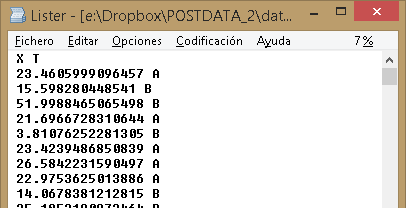
\includegraphics[width=10cm]{../fig/Tut09-08.png}
\end{center}

Para leer los datos del fichero usamos {\tt read.table} y comprobamos que la lectura ha sido correcta con {\tt head} así:
\begin{knitrout}
\definecolor{shadecolor}{rgb}{0.969, 0.969, 0.969}\color{fgcolor}\begin{kframe}
\begin{alltt}
\hlstd{datos} \hlkwb{=} \hlkwd{read.table}\hlstd{(}\hlstr{"../datos/Tut09-Ejemplos-ContrasteMedias-02.csv"}\hlstd{,} \hlkwc{header} \hlstd{=} \hlnum{TRUE}\hlstd{,} \hlkwc{sep} \hlstd{=} \hlstr{""}\hlstd{)}
\hlkwd{head}\hlstd{(datos)}
\end{alltt}
\begin{verbatim}
##         X T
## 1 23.4606 A
## 2 15.5983 B
## 3 51.9988 B
## 4 21.6967 A
## 5  3.8108 B
## 6 23.4239 A
\end{verbatim}
\end{kframe}
\end{knitrout}

La función {\tt z-test} de la librería {\tt BSDA} no es tan cómoda como las funciones {\tt t.test} o {\tt var.test}. En particular, con esta función no podemos usar una fórmula como \verb#X ~ T# para describir lo que queremos hacer. Así que vamos a hacer algo mucho más {\em ``manual''}. Definimos dos vectores que contienen los valores de $X$ para cada uno de los grupos (niveles) definidos por el factor {\tt T}:
\begin{knitrout}
\definecolor{shadecolor}{rgb}{0.969, 0.969, 0.969}\color{fgcolor}\begin{kframe}
\begin{alltt}
\hlstd{XA} \hlkwb{=} \hlstd{datos}\hlopt{$}\hlstd{X[datos}\hlopt{$}\hlstd{T}\hlopt{==}\hlstr{"A"}\hlstd{]}
\hlstd{XB} \hlkwb{=} \hlstd{datos}\hlopt{$}\hlstd{X[datos}\hlopt{$}\hlstd{T}\hlopt{==}\hlstr{"B"}\hlstd{]}
\end{alltt}
\end{kframe}
\end{knitrout}
Y ahora aplicamos así la función:
\begin{knitrout}
\definecolor{shadecolor}{rgb}{0.969, 0.969, 0.969}\color{fgcolor}\begin{kframe}
\begin{alltt}
\hlkwd{z.test}\hlstd{(}\hlkwc{x} \hlstd{= XA,} \hlkwc{y} \hlstd{= XB,} \hlkwc{alternative} \hlstd{=} \hlstr{"two.sided"}\hlstd{,} \hlkwc{sigma.x} \hlstd{=} \hlkwd{sd}\hlstd{(XA),} \hlkwc{sigma.y} \hlstd{=} \hlkwd{sd}\hlstd{(XB))}
\end{alltt}


{\ttfamily\noindent\bfseries\color{errorcolor}{\#\# Error in eval(expr, envir, enclos): no se pudo encontrar la función "{}z.test"{}}}\end{kframe}
\end{knitrout}
Fíjate que además debemos incluir las cuasidesviaciones típicas (calculadas con {\tt sd}), porque de lo contrario se produce un error, ya que la función no las calcula por defecto.

Con esto, hemos obtenido el p-valor del contraste. Es posible que te pregunte qué sucedería si, en lugar de {\tt z.test}, usáramos {\tt t.test} en este caso de muestras grandes. Y si la usamos, ¿debemos usar la opción de varianzas iguales o distintas?

\begin{ejercicio}
\label{tut09:ejercicio05}
Usa la función {\tt t.test} para realizar este contraste. Prueba las dos opciones posibles sobre las varianzas. ¿Cuál de ellas produce un resultado más parecido al que hemos obtenido con {\tt z.test}? ¿Qué sucede si, al usar {\tt t.test}, no indicas ninguna opción sobre la igualdad de las varianzas? Es decir, ¿cuál es el comportamiento {\em por defecto} de R?
Solución en la página \pageref{tut09:ejercicio05:sol}.
\qed
\end{ejercicio}

\subsubsection*{La función {\tt t.test} para datos emparejados.}

En la Sección \ref{curso-cap09:subsec:CasoDatosEmparejados} del libro (pág. \pageref{curso-cap09:subsec:CasoDatosEmparejados}) y también en este mismo tutorial, en la Sección \ref{tut09:subsec:DatosEmparejados1} (pág. \pageref{tut09:subsec:DatosEmparejados1}) hemos discutido el caso de los datos emparejados. Este tipo de contrastes, cuando disponemos de los datos {\em en bruto}, se llevan a cabo con mucha comodidad usando {\tt t.test}, con la opción {\tt paired=TRUE}.

Veamos un ejemplo. La librería {\tt BSDA}, que hemos usado antes, contiene un conjunto de datos, llamado {\tt Fitness}. Este conjunto de datos representa el número de un cierto tipo de flexiones que un grupo de sujetos podían hacer antes (en la columna {\em Before}) y después (columna {\em After}) de someterse a un programa de entrenamiento deportivo. Vamos a cargar ese conjunto de datos y a explorar su estructura:

\begin{knitrout}
\definecolor{shadecolor}{rgb}{0.969, 0.969, 0.969}\color{fgcolor}\begin{kframe}
\begin{alltt}
\hlkwd{library}\hlstd{(BSDA)}
\end{alltt}


{\ttfamily\noindent\bfseries\color{errorcolor}{\#\# Error in library(BSDA): there is no package called 'BSDA'}}\begin{alltt}
\hlkwd{data}\hlstd{(Fitness)}
\end{alltt}


{\ttfamily\noindent\color{warningcolor}{\#\# Warning in data(Fitness): data set 'Fitness' not found}}\begin{alltt}
\hlkwd{head}\hlstd{(Fitness)}
\end{alltt}


{\ttfamily\noindent\bfseries\color{errorcolor}{\#\# Error in head(Fitness): objeto 'Fitness' no encontrado}}\begin{alltt}
\hlkwd{str}\hlstd{(Fitness)}
\end{alltt}


{\ttfamily\noindent\bfseries\color{errorcolor}{\#\# Error in str(Fitness): objeto 'Fitness' no encontrado}}\end{kframe}
\end{knitrout}

Además de {\tt head} hemos usado la función {\tt str}, que puede ser de mucha utilidad en este tipo de exploraciones preliminares. Como ves, el conjunto de datos contiene $5$ observaciones, dos para cada individuo que se sometió al programa de entrenamiento. Por eso es un ejemplo típico de las situaciones que englobamos bajo esta etiqueta de {\em datos emparejados}. Llamando $\mu_a$ a la media antes del entrenamiento y $\mu_d$ a la media después del entrenamiento, queremos usar los datos para contrastar la hipótesis alternativa unilateral
\[H_a = \{\mu_a < \mu_d\}.\]
Y para hacer esto basta con usar {\tt t.test} así:

\begin{knitrout}
\definecolor{shadecolor}{rgb}{0.969, 0.969, 0.969}\color{fgcolor}\begin{kframe}
\begin{alltt}
\hlkwd{t.test}\hlstd{(Fitness}\hlopt{$}\hlstd{Before, Fitness}\hlopt{$}\hlstd{After,}
    \hlkwc{alternative} \hlstd{=} \hlstr{"less"}\hlstd{,} \hlkwc{paired} \hlstd{=} \hlnum{TRUE}\hlstd{,} \hlkwc{conf.level} \hlstd{=} \hlnum{0.95}\hlstd{)}
\end{alltt}


{\ttfamily\noindent\bfseries\color{errorcolor}{\#\# Error in t.test(Fitness\$Before, Fitness\$After, alternative = "{}less"{}, paired = TRUE, : objeto 'Fitness' no encontrado}}\end{kframe}
\end{knitrout}
La clave, por supuesto, es la opción {\tt paired=TRUE}. Fíjate, aparte de esto, en que el conjunto de datos no cumple el principio deseable de {\em una variable por columna, una observación por fila}. Por eso hemos usado la notación \verb#$# para acceder a las columnas {\tt Before} y {\tt After}.  La conclusión, es que al $95\%$ rechazamos $H_0$, pero no al $99\%$.
Con una muestra tan pequeña, eso significaría en la práctica, casi siempre, que los datos no son concluyentes. Se necesitan más datos: más potencia en el contraste, en el sentido que hemos discutido en el Capítulo \ref{curso-cap:ContrasteHipotesis}.

%\noindent{\bf Ejercicios:}
%\begin{itemize}
%  \item Interpreta este resultado de {\tt prop.test}. ¿Rechazamos la hipótesis nula?
%  \item Comprueba las cuentas del Ejemplo \ref{curso-cap09:ejem:ContrasteDiferenciaProporciones} (pág. \pageref{curso-cap09:ejem:ContrasteDiferenciaProporciones}) del curso. Asegúrate de incluir la opción {\tt correct=FALSE} en la llamada a {\tt prop.test}.
%\end{itemize}
%\qed


%\section{Riesgo relativo y cociente de posibilidades (odds ratio).}
%
%\textcolor{blue}{Próximamente se añadirá esta sección.}


\section{Ejercicios adicionales y soluciones.}
\label{tut09:sec:EjerciciosAdicionalesYSoluciones}

\subsection*{Ejercicios adicionales.}
\label{tut09:subsec:EjerciciosAdicionales}

Hemos usado R en todos los casos para obtener las soluciones de los siguientes ejercicios. Pero es recomendable que pruebes alguna de las otras herramientas a tu disposición, al menos en alguno de estos ejercicios.

\begin{ejercicio}
\label{tut09:ejercicio06}

Para hacer un contraste de proporciones en dos poblaciones disponemos de estos datos muestrales, procedentes de dos muestras aleatorias independientes tomadas respectivamente de cada una de esas dos poblaciones:
\[
\begin{cases}
n1=532, \mbox{número de {\em éxitos} en la primera muestra} = 197.\\
n2=486, \mbox{número de {\em éxitos} en la segunda muestra} = 151.\\
\end{cases}
\]
Usa estos datos para contrastar la hipótesis nula $H_0=\{p_1 = p_2\}$.
\qed
\end{ejercicio}

\begin{ejercicio}
\label{tut09:ejercicio07}








Para hacer un contraste de diferencia de medias de la variable $X$ entre dos poblaciones normales disponemos de estos datos muestrales, procedentes de dos muestras aleatorias independientes tomadas respectivamente de cada una de esas dos poblaciones:
\[
\begin{cases}
n_1 = 286,\\
{\bar X}_1 = 137.5\\
s_1 = 2.2
\end{cases}
\qquad\qquad
\begin{cases}
n_2 = 331,\\
{\bar X}_2 = 142.4\\
s_2 = 15.6
\end{cases}
\]
Usa estos datos para contrastar la hipótesis nula $H_0=\{\mu_1 \geq \mu_2 \}$.
Solución en la página \pageref{tut09:ejercicio07:sol}.
\qed
\end{ejercicio}


\begin{ejercicio}
\label{tut09:ejercicio08}




De nuevo, para hacer un contraste de diferencia de medias de la variable $X$ entre dos poblaciones normales disponemos de estos datos muestrales, procedentes de dos muestras aleatorias independientes tomadas respectivamente de cada una de esas dos poblaciones:
\[
\begin{cases}
n_1 = 12,\\
{\bar X}_1 = 45.3\\
s_1 = 3.7
\end{cases}
\qquad\qquad
\begin{cases}
n_2 = 14,\\
{\bar X}_2 = 40.4\\
s_2 = 3.9
\end{cases}
\]
Usa estos datos para contrastar la hipótesis nula $H_0=\{\mu_1 \leq \mu_2 \}$.
Solución en la página \pageref{tut09:ejercicio08:sol}.
\qed
\end{ejercicio}


\begin{ejercicio}
\label{tut09:ejercicio09}




Y por último, para hacer un contraste de diferencia de medias de la variable $X$ entre dos poblaciones normales disponemos de estos datos muestrales, procedentes de dos muestras aleatorias independientes tomadas respectivamente de cada una de esas dos poblaciones:
\[
\begin{cases}
n_1 = 7,\\
{\bar X}_1 = 0.9\\
s_1 = 0.96
\end{cases}
\qquad\qquad
\begin{cases}
n_2 = 7,\\
{\bar X}_2 = 1.2\\
s_2 = 0.27
\end{cases}
\]
Usa estos datos para contrastar la hipótesis nula $H_0=\{\mu_1 \geq \mu_2 \}$.
Solución en la página \pageref{tut09:ejercicio09:sol}.
\qed
\end{ejercicio}


%%##########################################
%##########################################

\subsection*{Soluciones de algunos ejercicios.}
\label{tut09:subsec:SolucionesAlgunosEjercicios}


\paragraph{\bf $\bullet$ Ejercicio \ref{tut09:ejercicio02}, pág. \pageref{tut09:ejercicio02}}
\label{tut09:ejercicio02:sol}\quad\\

\begin{enumerate}
  \item El código del fichero con los datos de este ejercicio aparece a continuación. Hemos descomentado las líneas donde aparecen los valores de $s_1$ y $s_2$ :

\begin{knitrout}
\definecolor{shadecolor}{rgb}{0.969, 0.969, 0.969}\color{fgcolor}\begin{kframe}
\begin{alltt}
    \hlcom{####################################################}
    \hlcom{# www.postdata-statistics.com}
    \hlcom{# POSTDATA. Introducción a la Estadísitica}
    \hlcom{# Tutorial-09.}
    \hlcom{#}
    \hlcom{# Fichero de instrucciones R para calcular}
    \hlcom{# un intervalo de confianza para la}
    \hlcom{# DIFERENCIA DE MEDIAS DE 2 POBLACIONES NORMALES}
    \hlcom{# usando la distribución Z}
    \hlcom{# Es el caso de MUESTRAS GRANDES o (poco frecuente)}
    \hlcom{# de varianzas poblacionales conocidas.}
    \hlcom{##############################################################}


    \hlkwd{rm}\hlstd{(}\hlkwc{list}\hlstd{=}\hlkwd{ls}\hlstd{())}

    \hlcom{# PRIMERA MUESTRA}
    \hlcom{# Numero de elementos}
    \hlstd{(n1} \hlkwb{=} \hlnum{245}\hlstd{)}
\end{alltt}
\begin{verbatim}
## [1] 245
\end{verbatim}
\begin{alltt}
    \hlcom{# Media muestral}
    \hlstd{(xbar1} \hlkwb{=} \hlnum{2.73}\hlstd{)}
\end{alltt}
\begin{verbatim}
## [1] 2.73
\end{verbatim}
\begin{alltt}
    \hlcom{# Cuasidesviacion tipica muestral o sigma (descomenta el que uses)}
    \hlstd{(s1} \hlkwb{=} \hlnum{0.4}\hlstd{)}
\end{alltt}
\begin{verbatim}
## [1] 0.4
\end{verbatim}
\begin{alltt}
    \hlcom{#(sigma1 = )}


    \hlcom{# SEGUNDA MUESTRA}
    \hlcom{# Numero de elementos}
    \hlstd{(n2} \hlkwb{=} \hlnum{252}\hlstd{)}
\end{alltt}
\begin{verbatim}
## [1] 252
\end{verbatim}
\begin{alltt}
    \hlcom{# Media muestral}
    \hlstd{(xbar2} \hlkwb{=} \hlnum{2.81}\hlstd{)}
\end{alltt}
\begin{verbatim}
## [1] 2.81
\end{verbatim}
\begin{alltt}
    \hlcom{# Cuasidesviacion tipica muestral o sigma (descomenta el que uses)}
    \hlstd{(s2} \hlkwb{=} \hlnum{0.3}\hlstd{)}
\end{alltt}
\begin{verbatim}
## [1] 0.3
\end{verbatim}
\begin{alltt}
    \hlcom{#(sigma2 = )}

    \hlcom{# Nivel de confianza deseado:}
    \hlstd{nc} \hlkwb{=} \hlnum{0.95}

    \hlcom{################################################}
    \hlcom{#NO CAMBIES NADA DE AQUI PARA ABAJO}
    \hlcom{################################################}

    \hlstd{(alfa} \hlkwb{=} \hlnum{1} \hlopt{-} \hlstd{nc)}
\end{alltt}
\begin{verbatim}
## [1] 0.05
\end{verbatim}
\begin{alltt}
    \hlcom{# Calculamos el valor critico:}
    \hlstd{(z_alfa2} \hlkwb{=} \hlkwd{qnorm}\hlstd{(} \hlnum{1} \hlopt{-} \hlstd{alfa} \hlopt{/} \hlnum{2}\hlstd{))}
\end{alltt}
\begin{verbatim}
## [1] 1.96
\end{verbatim}
\begin{alltt}
    \hlcom{# La diferencia de las medias muestrales es:}

    \hlstd{(xbar1} \hlopt{-} \hlstd{xbar2)}
\end{alltt}
\begin{verbatim}
## [1] -0.08
\end{verbatim}
\begin{alltt}
    \hlcom{# Comprobamos si se ha usado sigma como sustituto de s.}

    \hlkwa{if}\hlstd{(}\hlkwd{exists}\hlstd{(}\hlstr{"sigma1"}\hlstd{))\{s1} \hlkwb{=} \hlstd{sigma1\}}
    \hlkwa{if}\hlstd{(}\hlkwd{exists}\hlstd{(}\hlstr{"sigma2"}\hlstd{))\{s2} \hlkwb{=} \hlstd{sigma2\}}

    \hlcom{# La semianchura del intervalo es:}
    \hlstd{(semianchura} \hlkwb{=} \hlstd{z_alfa2} \hlopt{*} \hlkwd{sqrt}\hlstd{(s1}\hlopt{^}\hlnum{2}\hlopt{/}\hlstd{n1} \hlopt{+} \hlstd{s2}\hlopt{^}\hlnum{2}\hlopt{/}\hlstd{n2))}
\end{alltt}
\begin{verbatim}
## [1] 0.062295
\end{verbatim}
\begin{alltt}
    \hlcom{# El intervalo de confianza es este:}

    \hlstd{(intervalo} \hlkwb{=} \hlstd{xbar1} \hlopt{-} \hlstd{xbar2} \hlopt{+} \hlkwd{c}\hlstd{(}\hlopt{-}\hlnum{1}\hlstd{,} \hlnum{1}\hlstd{)} \hlopt{*} \hlstd{semianchura )}
\end{alltt}
\begin{verbatim}
## [1] -0.142295 -0.017705
\end{verbatim}
\end{kframe}
\end{knitrout}

  \item Esta es la forma de usar la {\em Calculadora de Probabilidades}:
    \begin{center}
    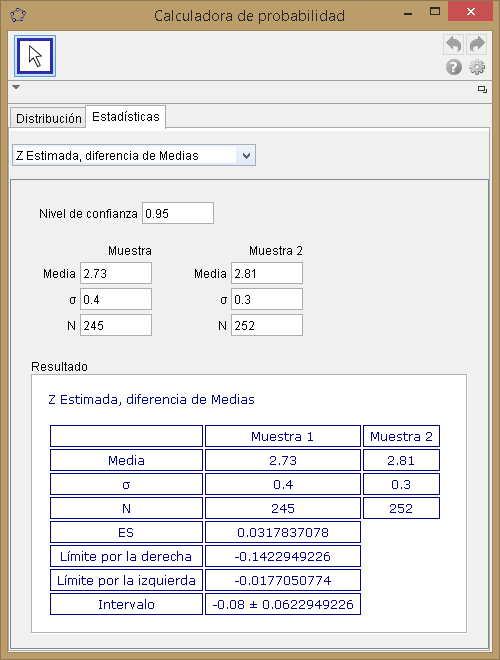
\includegraphics[width=11cm]{../fig/Tut09-09.png}
    \end{center}

  \item  En la siguiente figura se muestra como introducir ls datos para este ejercicio. Observa la forma de elegir entre muestras grandes y pequeñas, como indica la flecha roja.
    \begin{center}
    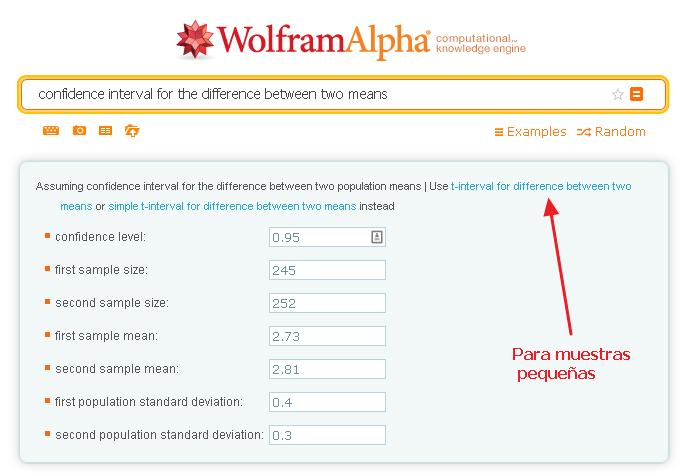
\includegraphics[width=14cm]{../fig/Tut09-15.png}
    \end{center}
    Y en esta figura puedes ver la salida de Wolfram Alpha:
    \begin{center}
    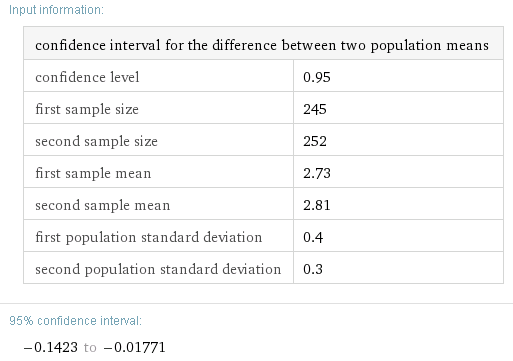
\includegraphics[width=14cm]{../fig/Tut09-16.png}
    \end{center}


  \item Introducimos los datos para el contraste en Wolfram Alpha como se muestra en la figura. Fíjate en las opciones que te permiten trabajar con muestras pequeñas, que hemos destacado con las flechas rojas:
    \begin{center}
    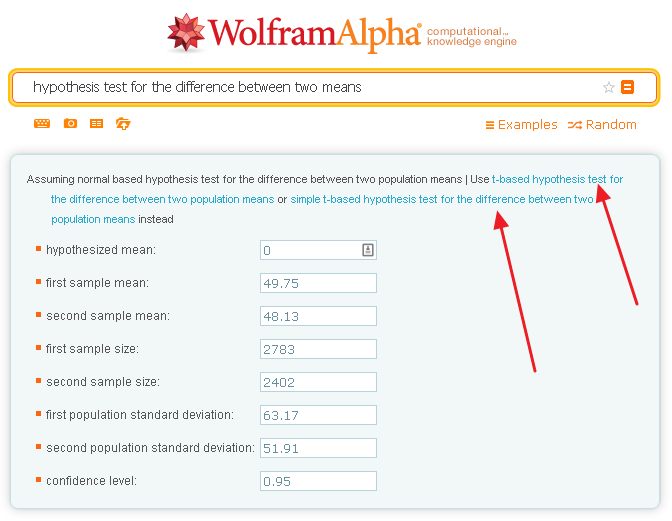
\includegraphics[width=14cm]{../fig/Tut09-10.png}
    \end{center}
    La respuesta que se obtiene es esta. Fíjate de nuevo en las opciones disponibles para usar contrastes unilaterales o bilaterales.
    \begin{center}
    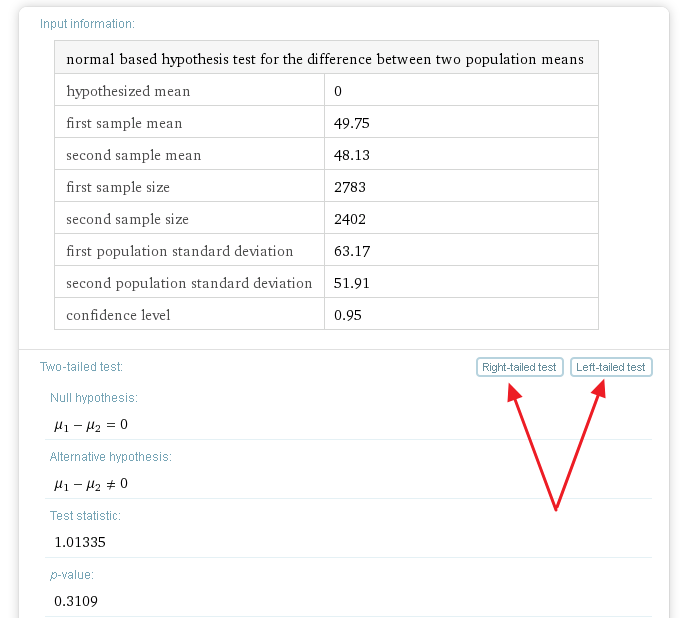
\includegraphics[width=14cm]{../fig/Tut09-11.png}
    \end{center}

    Para hacer el mismo contraste usando la plantilla de R llamada

     \begin{center}
     {\tt Tut09-Contraste-2Pob-DifMedias-UsandoZ.R}
     \end{center}
     introducimos los datos del ejemplo al principio del código. Recuerda descomentar las líneas de $s_1$ y $s_2$:
\begin{knitrout}
\definecolor{shadecolor}{rgb}{0.969, 0.969, 0.969}\color{fgcolor}\begin{kframe}
\begin{alltt}
  \hlcom{# PRIMERA MUESTRA}
  \hlcom{# Numero de elementos}
   \hlstd{(n1} \hlkwb{=} \hlnum{2783}\hlstd{)}
\end{alltt}
\begin{verbatim}
## [1] 2783
\end{verbatim}
\begin{alltt}
  \hlcom{# Media muestral}
   \hlstd{(xbar1} \hlkwb{=} \hlnum{49.75}\hlstd{)}
\end{alltt}
\begin{verbatim}
## [1] 49.75
\end{verbatim}
\begin{alltt}
  \hlcom{# Cuasidesviacion tipica muestral o sigma (descomenta el que uses)}
   \hlstd{(s1} \hlkwb{=} \hlnum{63.17}\hlstd{)}
\end{alltt}
\begin{verbatim}
## [1] 63.17
\end{verbatim}
\begin{alltt}
   \hlcom{#(sigma1 = )}


  \hlcom{# SEGUNDA MUESTRA}
  \hlcom{# Numero de elementos}
   \hlstd{(n2} \hlkwb{=} \hlnum{2402}\hlstd{)}
\end{alltt}
\begin{verbatim}
## [1] 2402
\end{verbatim}
\begin{alltt}
  \hlcom{# Media muestral}
   \hlstd{(xbar2} \hlkwb{=} \hlnum{48.13}\hlstd{)}
\end{alltt}
\begin{verbatim}
## [1] 48.13
\end{verbatim}
\begin{alltt}
  \hlcom{# Cuasidesviacion tipica muestral o sigma (descomenta el que uses)}
   \hlstd{(s2} \hlkwb{=} \hlnum{51.91}\hlstd{)}
\end{alltt}
\begin{verbatim}
## [1] 51.91
\end{verbatim}
\begin{alltt}
   \hlcom{#(sigma2 = )}

  \hlcom{# ¿Que tipo de contraste estamos haciendo?}
  \hlcom{# Escribe 1 si la HIP. ALTERNATIVA es mu1 > mu2,}
  \hlcom{#         2 si es mu1 < mu2,}
  \hlcom{#         3 si es mu1 distinto de mu2}
  \hlstd{TipoContraste} \hlkwb{=} \hlnum{3}

  \hlcom{#Nivel de significacion}
   \hlstd{(nSig} \hlkwb{=} \hlnum{0.95}\hlstd{)}
\end{alltt}
\begin{verbatim}
## [1] 0.95
\end{verbatim}
\end{kframe}
\end{knitrout}


Y los resultados que se obtienen coinciden, como cabía esperar con  los de Wolfram Alpha.
\begin{knitrout}
\definecolor{shadecolor}{rgb}{0.969, 0.969, 0.969}\color{fgcolor}\begin{kframe}
\begin{alltt}
      \hlkwd{pValor}\hlstd{(Estadistico, TipoContraste)}
\end{alltt}
\begin{verbatim}
## [1] "El p-Valor es 0.31089244301084"
\end{verbatim}
\begin{alltt}
      \hlstd{Estadistico}
\end{alltt}
\begin{verbatim}
## [1] 1.0134
\end{verbatim}
\begin{alltt}
      \hlkwd{RegionRechazo}\hlstd{(alfa, TipoContraste)}
\end{alltt}
\begin{verbatim}
## [1] "La region de rechazo la forman los Valores del Estadistico mas alejados del origen que  1.95996398454005"
\end{verbatim}
\end{kframe}
\end{knitrout}



\end{enumerate}

\paragraph{\bf $\bullet$ Ejercicio \ref{tut09:ejercicio03}, pág. \pageref{tut09:ejercicio03}}
\label{tut09:ejercicio03:sol}\quad\\

Las siguientes figuras muestran la solución de ambos problemas de probabilidad:

    \begin{center}
    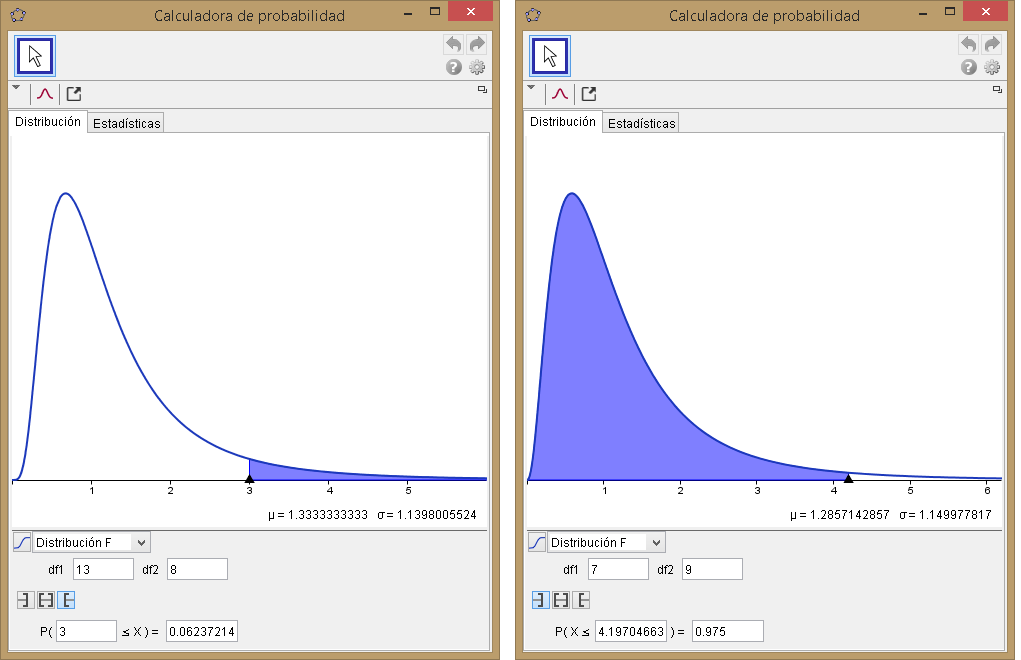
\includegraphics[width=16cm]{../fig/Tut09-12.png}
    \end{center}

\paragraph{\bf $\bullet$ Ejercicio \ref{tut09:ejercicio04}, pág. \pageref{tut09:ejercicio04}}
\label{tut09:ejercicio04:sol}\quad\\

El código R para leer el fichero es:
\begin{knitrout}
\definecolor{shadecolor}{rgb}{0.969, 0.969, 0.969}\color{fgcolor}\begin{kframe}
\begin{alltt}
 \hlstd{datos} \hlkwb{=} \hlkwd{read.table}\hlstd{(}\hlstr{"../datos/Tut09-Ejemplos-ContrasteMedias-01.csv"}\hlstd{,} \hlkwc{header} \hlstd{=} \hlnum{TRUE}\hlstd{,} \hlkwc{sep} \hlstd{=} \hlstr{""}\hlstd{)}
 \hlkwd{head}\hlstd{(datos)}
\end{alltt}
\begin{verbatim}
##        X T
## 1 4.3056 A
## 2 6.5297 A
## 3 6.0386 A
## 4 9.1185 A
## 5 2.4946 A
## 6 6.5334 A
\end{verbatim}
\begin{alltt}
 \hlkwd{tail}\hlstd{(datos)}
\end{alltt}
\begin{verbatim}
##           X T
## 23 10.87338 B
## 24 -6.60762 B
## 25 -2.71845 B
## 26 21.50246 B
## 27 17.35569 B
## 28 -0.18161 B
\end{verbatim}
\end{kframe}
\end{knitrout}
Ahora podemos hacer el contraste de igualdad de varianzas en una sola línea de código:
\begin{knitrout}
\definecolor{shadecolor}{rgb}{0.969, 0.969, 0.969}\color{fgcolor}\begin{kframe}
\begin{alltt}
\hlkwd{var.test}\hlstd{(X} \hlopt{~} \hlstd{T,} \hlkwc{data} \hlstd{= datos,} \hlkwc{alternative} \hlstd{=} \hlstr{"two.sided"}\hlstd{,} \hlkwc{conf.level} \hlstd{=} \hlnum{0.95}\hlstd{)}
\end{alltt}
\begin{verbatim}
## 
## 	F test to compare two variances
## 
## data:  X by T
## F = 0.056, num df = 11, denom df = 15, p-value = 0.000027
## alternative hypothesis: true ratio of variances is not equal to 1
## 95 percent confidence interval:
##  0.018605 0.186344
## sample estimates:
## ratio of variances 
##            0.05596
\end{verbatim}
\end{kframe}
\end{knitrout}
El p-valor obtenido nos lleva a rechazar la hipótesis nula de varianzas iguales. Así que podemos hacer el contraste de igualdad de medias, teniendo en cuenta este resultado para elegir el valor de la opción {\tt var.equal} de {\tt t.test}:
\begin{knitrout}
\definecolor{shadecolor}{rgb}{0.969, 0.969, 0.969}\color{fgcolor}\begin{kframe}
\begin{alltt}
\hlkwd{t.test}\hlstd{(X} \hlopt{~} \hlstd{T,} \hlkwc{data} \hlstd{= datos,}
    \hlkwc{alternative} \hlstd{=} \hlstr{"two.sided"}\hlstd{,} \hlkwc{conf.level} \hlstd{=} \hlnum{0.95}\hlstd{,} \hlkwc{var.equal}\hlstd{=}\hlnum{FALSE}\hlstd{)}
\end{alltt}
\begin{verbatim}
## 
## 	Welch Two Sample t-test
## 
## data:  X by T
## t = 1.58, df = 17.2, p-value = 0.13
## alternative hypothesis: true difference in means is not equal to 0
## 95 percent confidence interval:
##  -1.2807  8.8807
## sample estimates:
## mean in group A mean in group B 
##             6.7             2.9
\end{verbatim}
\end{kframe}
\end{knitrout}
El p-valor que hemos obtenido indica que debemos rechazar la hipótesis alternativa,y concluir que no hay evidencia basada en los datos para creer que las medias de ambas poblaciones sean distintas.


\paragraph{\bf $\bullet$ Ejercicio \ref{tut09:ejercicio05}, pág. \pageref{tut09:ejercicio05}}
\label{tut09:ejercicio05:sol}\quad\\

Vamos a recordar primero el contraste con $Z$:
\begin{knitrout}
\definecolor{shadecolor}{rgb}{0.969, 0.969, 0.969}\color{fgcolor}\begin{kframe}
\begin{alltt}
\hlstd{datos} \hlkwb{=} \hlkwd{read.table}\hlstd{(}\hlstr{"../datos/Tut09-Ejemplos-ContrasteMedias-02.csv"}\hlstd{,} \hlkwc{header} \hlstd{=} \hlnum{TRUE}\hlstd{,} \hlkwc{sep} \hlstd{=} \hlstr{""}\hlstd{)}
\hlstd{XA} \hlkwb{=} \hlstd{datos}\hlopt{$}\hlstd{X[datos}\hlopt{$}\hlstd{T}\hlopt{==}\hlstr{"A"}\hlstd{]}
\hlstd{XB} \hlkwb{=} \hlstd{datos}\hlopt{$}\hlstd{X[datos}\hlopt{$}\hlstd{T}\hlopt{==}\hlstr{"B"}\hlstd{]}
\hlkwd{z.test}\hlstd{(}\hlkwc{x} \hlstd{= XA,} \hlkwc{y} \hlstd{= XB,} \hlkwc{alternative} \hlstd{=} \hlstr{"two.sided"}\hlstd{,} \hlkwc{sigma.x} \hlstd{=} \hlkwd{sd}\hlstd{(XA),} \hlkwc{sigma.y} \hlstd{=} \hlkwd{sd}\hlstd{(XB))}
\end{alltt}


{\ttfamily\noindent\bfseries\color{errorcolor}{\#\# Error in eval(expr, envir, enclos): no se pudo encontrar la función "{}z.test"{}}}\end{kframe}
\end{knitrout}
Y ahora veamos las tres posibilidades con $t$:
\begin{knitrout}
\definecolor{shadecolor}{rgb}{0.969, 0.969, 0.969}\color{fgcolor}\begin{kframe}
\begin{alltt}
\hlkwd{t.test}\hlstd{(}\hlkwc{x} \hlstd{= XA,} \hlkwc{y} \hlstd{= XB,} \hlkwc{alternative} \hlstd{=} \hlstr{"two.sided"}\hlstd{,} \hlkwc{var.equal}\hlstd{=}\hlnum{FALSE}\hlstd{)}
\end{alltt}
\begin{verbatim}
## 
## 	Welch Two Sample t-test
## 
## data:  XA and XB
## t = -3.22, df = 295, p-value = 0.0014
## alternative hypothesis: true difference in means is not equal to 0
## 95 percent confidence interval:
##  -4.8313 -1.1687
## sample estimates:
## mean of x mean of y 
##        23        26
\end{verbatim}
\begin{alltt}
\hlkwd{t.test}\hlstd{(}\hlkwc{x} \hlstd{= XA,} \hlkwc{y} \hlstd{= XB,} \hlkwc{alternative} \hlstd{=} \hlstr{"two.sided"}\hlstd{,} \hlkwc{var.equal}\hlstd{=}\hlnum{TRUE}\hlstd{)}
\end{alltt}
\begin{verbatim}
## 
## 	Two Sample t-test
## 
## data:  XA and XB
## t = -3.42, df = 607, p-value = 0.00067
## alternative hypothesis: true difference in means is not equal to 0
## 95 percent confidence interval:
##  -4.7235 -1.2765
## sample estimates:
## mean of x mean of y 
##        23        26
\end{verbatim}
\begin{alltt}
\hlkwd{t.test}\hlstd{(}\hlkwc{x} \hlstd{= XA,} \hlkwc{y} \hlstd{= XB,} \hlkwc{alternative} \hlstd{=} \hlstr{"two.sided"}\hlstd{)}
\end{alltt}
\begin{verbatim}
## 
## 	Welch Two Sample t-test
## 
## data:  XA and XB
## t = -3.22, df = 295, p-value = 0.0014
## alternative hypothesis: true difference in means is not equal to 0
## 95 percent confidence interval:
##  -4.8313 -1.1687
## sample estimates:
## mean of x mean of y 
##        23        26
\end{verbatim}
\end{kframe}
\end{knitrout}

Como ves, la más parecida es aquella en la primera, en la que suponemos que las varianzas son distintas y que es, además, la opción por defecto que usa R.


\paragraph{\bf $\bullet$ Ejercicio \ref{tut09:ejercicio06}, pág. \pageref{tut09:ejercicio06}}
\label{tut09:ejercicio06:sol}\quad\\


Podemos usar así la función {\tt prop.test}:
\begin{knitrout}
\definecolor{shadecolor}{rgb}{0.969, 0.969, 0.969}\color{fgcolor}\begin{kframe}
\begin{alltt}
\hlkwd{prop.test}\hlstd{(}\hlkwd{c}\hlstd{(}\hlnum{197}\hlstd{,}\hlnum{151}\hlstd{),}\hlkwc{n}\hlstd{=}\hlkwd{c}\hlstd{(}\hlnum{532}\hlstd{,}\hlnum{486}\hlstd{),}\hlkwc{alternative}\hlstd{=}\hlstr{"two.sided"}\hlstd{,}\hlkwc{conf.level}\hlstd{=}\hlnum{0.95}\hlstd{,}\hlkwc{correct}\hlstd{=}\hlnum{FALSE}\hlstd{)}
\end{alltt}
\begin{verbatim}
## 
## 	2-sample test for equality of proportions without continuity
## 	correction
## 
## data:  c(197, 151) out of c(532, 486)
## X-squared = 4.01, df = 1, p-value = 0.045
## alternative hypothesis: two.sided
## 95 percent confidence interval:
##  0.0014931 0.1177092
## sample estimates:
## prop 1 prop 2 
## 0.3703 0.3107
\end{verbatim}
\end{kframe}
\end{knitrout}
Como puedes ver, hemos usado la opción {\tt correct=FALSE}, para evitar que R use una corrección de continuidad en la aproximación normal a la binomial. De esa forma, y aunque perdamos un poco de precisión, tratamos de obtener los resultados a los que conduce el estadístico que aparece en la Ecuación \ref{curso-cap09:ecu:EstadisticoDiferencia2Proporciones}  (pág. \pageref{curso-cap09:ecu:EstadisticoDiferencia2Proporciones}) del Capítulo \ref{curso-cap:Inferencia2Poblaciones} del libro.


\paragraph{\bf $\bullet$ Ejercicio \ref{tut09:ejercicio07}, pág. \pageref{tut09:ejercicio07}}
\label{tut09:ejercicio07:sol}\quad\\

Este es el código de la plantilla de R con los datos del ejercicio:

\begin{knitrout}
\definecolor{shadecolor}{rgb}{0.969, 0.969, 0.969}\color{fgcolor}\begin{kframe}
\begin{alltt}
  \hlcom{# PRIMERA MUESTRA}
  \hlcom{# Numero de elementos}
      \hlstd{(n1} \hlkwb{=} \hlnum{286}\hlstd{)}
\end{alltt}
\begin{verbatim}
## [1] 286
\end{verbatim}
\begin{alltt}
  \hlcom{# Media muestral}
      \hlstd{(xbar1} \hlkwb{=} \hlnum{137.5}\hlstd{)}
\end{alltt}
\begin{verbatim}
## [1] 137.5
\end{verbatim}
\begin{alltt}
  \hlcom{# Cuasidesviacion tipica muestral o sigma (descomenta el que uses)}
      \hlstd{(s1} \hlkwb{=} \hlnum{15.6}\hlstd{)}
\end{alltt}
\begin{verbatim}
## [1] 15.6
\end{verbatim}
\begin{alltt}
      \hlcom{#(sigma1 = )}


  \hlcom{# SEGUNDA MUESTRA}
  \hlcom{# Numero de elementos}
      \hlstd{(n2} \hlkwb{=} \hlnum{331}\hlstd{)}
\end{alltt}
\begin{verbatim}
## [1] 331
\end{verbatim}
\begin{alltt}
  \hlcom{# Media muestral}
      \hlstd{(xbar2} \hlkwb{=} \hlnum{142.4}\hlstd{)}
\end{alltt}
\begin{verbatim}
## [1] 142.4
\end{verbatim}
\begin{alltt}
  \hlcom{# Cuasidesviacion tipica muestral o sigma (descomenta el que uses)}
      \hlstd{(s2} \hlkwb{=} \hlnum{19.4}\hlstd{)}
\end{alltt}
\begin{verbatim}
## [1] 19.4
\end{verbatim}
\begin{alltt}
      \hlcom{#(sigma2 = )}

\hlcom{# ¿Que tipo de contraste estamos haciendo?}
\hlcom{# Escribe 1 si la HIP. ALTERNATIVA es mu1 > mu2,}
\hlcom{#         2 si es mu1 < mu2,}
\hlcom{#         3 si es mu1 distinto de mu2}
      \hlstd{TipoContraste} \hlkwb{=} \hlnum{2}
  \hlcom{#Nivel de significacion}
      \hlstd{(nSig} \hlkwb{=} \hlnum{0.95}\hlstd{)}
\end{alltt}
\begin{verbatim}
## [1] 0.95
\end{verbatim}
\end{kframe}
\end{knitrout}


Y los resultados que se obtienen son:
\begin{knitrout}
\definecolor{shadecolor}{rgb}{0.969, 0.969, 0.969}\color{fgcolor}\begin{kframe}
\begin{alltt}
      \hlkwd{pValor}\hlstd{(Estadistico, TipoContraste)}
\end{alltt}
\begin{verbatim}
## [1] "El p-Valor es 0.000255131809259936"
\end{verbatim}
\begin{alltt}
      \hlstd{Estadistico}
\end{alltt}
\begin{verbatim}
## [1] -3.4753
\end{verbatim}
\end{kframe}
\end{knitrout}


\paragraph{\bf $\bullet$ Ejercicio \ref{tut09:ejercicio08}, pág. \pageref{tut09:ejercicio08}}
\label{tut09:ejercicio08:sol}\quad\\



Al tratarse de un contraste de diferencia de medias con muestras pequeñas debemos usar la $t$ de Student y, previamente, para ello debemos hacer un contraste de la hipótesis nula de igualdad de varianzas:
\[H_0 = \{\sigma_1 ^2 = \sigma^2_2\}\]
El estadístico de este contraste es
\begin{knitrout}
\definecolor{shadecolor}{rgb}{0.969, 0.969, 0.969}\color{fgcolor}\begin{kframe}
\begin{alltt}
\hlstd{(EstadisticoVar} \hlkwb{=} \hlstd{s1}\hlopt{^}\hlnum{2}\hlopt{/}\hlstd{s2}\hlopt{^}\hlnum{2}\hlstd{)}
\end{alltt}
\begin{verbatim}
## [1] 0.90007
\end{verbatim}
\end{kframe}
\end{knitrout}
Y, puesto que este estadístico es menor que $1$, usamos la cola izquierda de la distribución de Fisher para calcular el p-valor:
\begin{knitrout}
\definecolor{shadecolor}{rgb}{0.969, 0.969, 0.969}\color{fgcolor}\begin{kframe}
\begin{alltt}
\hlstd{(pValorVar} \hlkwb{=} \hlkwd{pf}\hlstd{(EstadisticoVar,} \hlkwc{df1} \hlstd{= n1} \hlopt{-} \hlnum{1}\hlstd{,} \hlkwc{df2} \hlstd{= n2} \hlopt{-} \hlnum{1}\hlstd{))}
\end{alltt}
\begin{verbatim}
## [1] 0.43589
\end{verbatim}
\end{kframe}
\end{knitrout}
Puedes calcularlo igualmente con la {\em Calculadora de Probabilidades} de GeoGebra, como en la figura:
    \begin{center}
    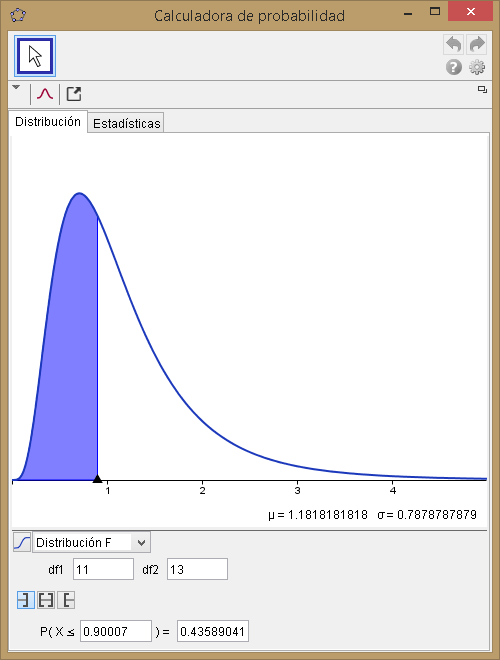
\includegraphics[width=9cm]{../fig/Tut09-14.png}
    \end{center}

Con este p-valor rechazamos la hipótesis alternativa de que las varianzas sean distintas. Teniendo esto en cuenta, volvamos al contraste sobre la diferencia de medias. Esta es la parte inicial del código de la plantilla de R
\begin{center}
  {\tt Tut09-Contraste-2Pob-DifMedias-UsandoT-VarIguales.R}
\end{center}
con los datos del ejercicio:
\begin{knitrout}
\definecolor{shadecolor}{rgb}{0.969, 0.969, 0.969}\color{fgcolor}\begin{kframe}
\begin{alltt}
 \hlcom{# PRIMERA MUESTRA # Numero de elementos}
 \hlstd{(n1} \hlkwb{=} \hlnum{12}\hlstd{)}
\end{alltt}
\begin{verbatim}
## [1] 12
\end{verbatim}
\begin{alltt}
 \hlcom{# Media muestral}
 \hlstd{(xbar1} \hlkwb{=} \hlnum{45.3}\hlstd{)}
\end{alltt}
\begin{verbatim}
## [1] 45.3
\end{verbatim}
\begin{alltt}
 \hlcom{# Cuasidesviacion tipica muestral}
 \hlstd{(s1} \hlkwb{=} \hlnum{3.7}\hlstd{)}
\end{alltt}
\begin{verbatim}
## [1] 3.7
\end{verbatim}
\begin{alltt}
 \hlcom{# SEGUNDA MUESTRA}
 \hlcom{# Numero de elementos}
 \hlstd{(n2} \hlkwb{=} \hlnum{14}\hlstd{)}
\end{alltt}
\begin{verbatim}
## [1] 14
\end{verbatim}
\begin{alltt}
 \hlcom{# Media muestral}
 \hlstd{(xbar2} \hlkwb{=} \hlnum{40.4}\hlstd{)}
\end{alltt}
\begin{verbatim}
## [1] 40.4
\end{verbatim}
\begin{alltt}
 \hlcom{# Cuasidesviacion tipica  muestral}
 \hlstd{(s2} \hlkwb{=} \hlnum{3.9}\hlstd{)}
\end{alltt}
\begin{verbatim}
## [1] 3.9
\end{verbatim}
\begin{alltt}
 \hlcom{# ¿Que tipo de contraste estamos haciendo?}
 \hlcom{# Escribe 1 si la HIP. ALTERNATIVA es mu1 > mu2, 2 si es mu1 < mu2, 3 si es mu1 distinto de mu2}
   \hlstd{TipoContraste} \hlkwb{=} \hlnum{1}
 \hlcom{#Nivel de significacion}
   \hlstd{(nSig} \hlkwb{=} \hlnum{0.95}\hlstd{)}
\end{alltt}
\begin{verbatim}
## [1] 0.95
\end{verbatim}
\end{kframe}
\end{knitrout}



Y los resultados que se obtienen son:
\begin{knitrout}
\definecolor{shadecolor}{rgb}{0.969, 0.969, 0.969}\color{fgcolor}\begin{kframe}
\begin{alltt}
     \hlkwd{pValor}\hlstd{(Estadistico, TipoContraste)}
\end{alltt}
\begin{verbatim}
## [1] "El p-Valor es 0.0015847637376516"
\end{verbatim}
\begin{alltt}
     \hlstd{Estadistico}
\end{alltt}
\begin{verbatim}
## [1] 3.2833
\end{verbatim}
\end{kframe}
\end{knitrout}
La conclusión es que rechazamos la hipótesis nula: los datos no permiten afirmar que sea $\mu_1\geq \mu_2$

\paragraph{\bf $\bullet$ Ejercicio \ref{tut09:ejercicio09}, pág. \pageref{tut09:ejercicio09}}
\label{tut09:ejercicio09:sol}\quad\\



De nuevo, puesto que las muestras son pequeñas debemos usar la $t$ de Student y eso nos lleva a empezar  con un contraste de la hipótesis nula de igualdad de varianzas:
\[H_0 = \{\sigma_1 ^2 = \sigma^2_2\}\]
El estadístico de este contraste vale, en este caso
\begin{knitrout}
\definecolor{shadecolor}{rgb}{0.969, 0.969, 0.969}\color{fgcolor}\begin{kframe}
\begin{alltt}
\hlstd{(EstadisticoVar} \hlkwb{=} \hlstd{s1}\hlopt{^}\hlnum{2}\hlopt{/}\hlstd{s2}\hlopt{^}\hlnum{2}\hlstd{)}
\end{alltt}
\begin{verbatim}
## [1] 12.642
\end{verbatim}
\end{kframe}
\end{knitrout}
Y, puesto que este estadístico es mayor que $1$, usamos la cola derecha de la distribución de Fisher para calcular el p-valor:
\begin{knitrout}
\definecolor{shadecolor}{rgb}{0.969, 0.969, 0.969}\color{fgcolor}\begin{kframe}
\begin{alltt}
\hlstd{(pValorVar} \hlkwb{=} \hlnum{1} \hlopt{-} \hlkwd{pf}\hlstd{(EstadisticoVar,} \hlkwc{df1} \hlstd{= n1} \hlopt{-} \hlnum{1}\hlstd{,} \hlkwc{df2} \hlstd{= n2} \hlopt{-} \hlnum{1}\hlstd{))}
\end{alltt}
\begin{verbatim}
## [1] 0.0035184
\end{verbatim}
\end{kframe}
\end{knitrout}
También puedes calcularlo con GeoGebra, desde luego:
    \begin{center}
    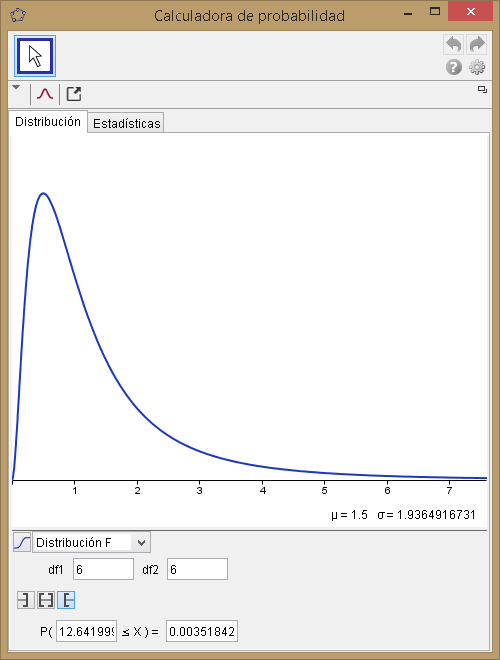
\includegraphics[width=9cm]{../fig/Tut09-13.png}
    \end{center}
Con este p-valor rechazamos la hipótesis nula de que las varianzas sean iguales. Usamos esto para decidir lo que hay que hacer en el contraste sobre la diferencia de medias. Este es el código de la plantilla de R
\begin{center}
  {\tt Tut09-Contraste-2Pob-DifMedias-UsandoT-VarDistintas.R}
\end{center}
con los datos del ejercicio:


Y los resultados que se obtienen son:
\begin{knitrout}
\definecolor{shadecolor}{rgb}{0.969, 0.969, 0.969}\color{fgcolor}\begin{kframe}
\begin{alltt}
     \hlkwd{pValor}\hlstd{(Estadistico, TipoContraste)}
\end{alltt}
\begin{verbatim}
## [1] "El p-Valor es 0.22621403141095"
\end{verbatim}
\begin{alltt}
     \hlstd{Estadistico}
\end{alltt}
\begin{verbatim}
## [1] -0.79592
\end{verbatim}
\end{kframe}
\end{knitrout}
La conclusión es que rechazamos la hipótesis alternativa: los datos no permiten afirmar que sea $\mu_1<\mu_2$



\newpage

\section*{Plantillas de R para contrastes e intervalos de confianza.}
\addcontentsline{toc}{section}{\textcolor{red}{PLANTILLAS DE R PARA CONTRASTES E INTERVALOS DE CONFIANZA.}}

\begin{table}[h!]

\framebox[14cm][l]{
\hspace{-3mm}
\begin{minipage}{13.5cm}
\begin{itemize}
  \item \textbf{Diferencia medias.}
        \begin{itemize}
          \item Usando $Z$.\\
              \fichero{./code/Tut09-Contraste-2Pob-DifMedias-UsandoZ.R}{Tut09-Contraste-2Pob-DifMedias-UsandoZ.R}\\
              \fichero{./code/Tut09-IntConf-2Pob-DifMedias-UsandoZ.R}{Tut09-IntConf-2Pob-DifMedias-UsandoZ.R}
          \item Usando la $t$ de Student.
              \begin{itemize}
                \item Varianzas desconocidas pero iguales.\\
                    \fichero{./code/Tut09-Contraste-2Pob-DifMedias-UsandoT-VarIguales.R}{Tut09-Contraste-2Pob-DifMedias-UsandoT-VarIguales.R}\\
                    \fichero{./code/Tut09-IntConf-2Pob-DifMedias-UsandoT-VarianzasIguales.R}{Tut09-IntConf-2Pob-DifMedias-UsandoT-VarianzasIguales.R}
                \item Varianzas desconocidas pero distintas.\\
                    \fichero{./code/Tut09-Contraste-2Pob-DifMedias-UsandoT-VarDistintas.R}{Tut09-Contraste-2Pob-DifMedias-UsandoT-VarDistintas.R}\\
                    \fichero{./code/Tut09-IntConf-2Pob-DifMedias-UsandoT-VarianzasDistintas.R}{Tut09-IntConf-2Pob-DifMedias-UsandoT-VarianzasDistintas.R}
              \end{itemize}
        \end{itemize}

  \item \textbf{Cociente varianzas.}\\
        \fichero{./code/Tut09-Contraste-2Pob-CocienteVarianzas.R}{Tut09-Contraste-2Pob-CocienteVarianzas.R}\\
        \fichero{./code/Tut09-IntConf-2Pob-CocienteVarianzas.R}{Tut09-IntConf-2Pob-CocienteVarianzas.R}

  \item \textbf{Diferencia proporciones.}\\
        \fichero{./code/Tut09-Contraste-2Pob-DifProporciones-UsandoZ.R}{Tut09-Contraste-2Pob-DifProporciones-UsandoZ.R}\\
        \fichero{./code/Tut09-IntConf-2Pob-DifProporciones-UsandoZ.R}{Tut09-IntConf-2Pob-DifProporciones-UsandoZ.R}
\end{itemize}
\end{minipage}
}
\caption{Ficheros para los contrastes de hipótesis e intervalos de confianza en dos poblaciones independientes.}
\label{Tut09:tabla:FicherosContrastesDosPoblaciones}
\end{table}


%#########################################################################################
%#########################################################################################
\vspace{2cm} \hrule
\quad\\
Fin del Tutorial09. ¡Gracias por la atención!





\end{document}



